% siminos/spatiotemp/chapter/catMapLatt.tex
% $Author: predrag $ $Date: 2021-12-08 00:39:15 -0500 (Wed, 08 Dec 2021) $

% called by siminos/spatiotemp/blogCats.tex

\Chapter{catMapLatt}{5jan2021}{{\catLatt}}
% \label{c-catMapLatt}  % formatted for ChaosBook.org
\renewcommand{\ssp}{x}

\begin{description}
\item[2016-09-09 Predrag]
I have added this chapter with intention to include it as several examples
in ChaosBook.org.

\item[2020-12-16 Predrag] The abstract of my online
Mathematical Physics Webinar,
Rutgers University - the most attended of the series :)

        \item[\videoLink{YouTube.com/embed/%
9r7wJroEVSA}]  {\em % uploaded              2020-09-22
Spatiotemporal cat - a chaotic field theory
         }
(55 min seminar)

     When I refer to a physical phenomenon -such as motions of a Navier-Stokes fluid- as `chaotic', or `turbulent', I am often told: We understand `chaos' for a system such as Lorenz attractor, but what is a `chaotic' field, a field with infinitely many degrees of freedom?

     The goal of the seminar is to answer this question pedagogically, as a sequence of pencil and paper calculations. First I will explain what is 'deterministic chaos' by walking you through its simplest example, the coin toss or Bernoulli map, but reformulated as problem of enumerating admissible global solutions on an integer-time lattice. Then I will do the same with the 'kicked rotor', the simplest mechanical system that is chaotic. Finally, I will take an infinity of `rotors' coupled together on a spatial lattice to explain what `chaos' or `turbulence' looks like in the spacetime.

      What emerges is a spacetime which is very much like a big spring mattress that obeys the familiar harmonic oscillator field theory equations, the discrete Helmholtz equation (or the tight-binding model), but instead of being `springy', this metamaterial is a dicretization of the Euclidean Klein-Gordon equation, with an unstable rotor at every lattice site, that gives, rather than pushes back, a theory formulated in terms of Hill determinants and zeta functions. We call this mother of all chaotic field theories the `spatiotemporal cat'.

      This is the simplest example of reformulating a space and time translationally invariant, exponentially unstable `turbulent' field theory as a (D+1)-dimensional spatiotemporal system which treats space and time on equal footing. Here there is no `evolution in time': there is only the enumeration of the repertoire of admissible tilings of spacetime by invariant (D+1)-dimensional tori, or `periodic orbits', very much as the partition function of the Ising model is a weighted sum formed by enumerating its lattice states. But that is a story for another seminar.
\\

 And if you don't know,
\HREF{https://www.youtube.com/watch?v=_JZom_gVfuw} {now you know}


\end{description}

%%%%%%%%%%%%%%%%%%%%%%%%%%%%%%%%%%%%%%%%%%%%%%%%
% siminos/spatiotemp/chapter/CML.tex
% $Author: predrag $ $Date: 2021-12-08 16:28:14 -0500 (Wed, 08 Dec 2021) $

% called by siminos/spatiotemp/chapter/catMapLatt.tex

\section{Coupled map lattices}
\label{s:CML}

Diffusive coupled map lattices (CML) were introduced by
Kaneko\rf{Kaneko83,Kaneko84}:
\beq
x_{n, t+1}=g(x_{n,t}) + \frac{\epsilon}{2}
            [
            g(x_{n-1,t}) - 2g(x_{n,t}) + g(x_{n+1,t})
            ]
          = (1+\epsilon\,\Box) g(x_{n,t})
\ee{KanekoCML}
where the individual site dynamical system $g(x)$ is a 1D map such as the
logistic map.


In the discretization of a spacetime field $q(x,t)$ on lattice points
$(x_n,t_j)$, the field is replaced by its lattice point value
$q_{n,j}= q(x_n,t_j)$. For a Hamiltonian set of fields we also have
$p_{n,j}= p(x_n,t_j)$.
In the {\catlatt}, a cat map at each  periodic lattice site
is coupled diffusively to its nearest neighbors:
\bea
q_{n, j+1}&=&p_{n,j}+(s-3)q_{n,j} - (q_{n+1,j} - 2q_{n,j} + q_{n-1,j}) - {m}^q_{n,j+1}
\continue
p_{n,j+1}&=&p_{n,j} + (s-4) q_{n,j} - (q_{n+1,j} - 2q_{n,j} + q_{n-1,j}) - {m}^p_{n,j+1}
\label{HamEqs}
\eea
The spatiotemporal symbols follow from the Newtonian equations
in $d$ spatiotemporal dimensions
\bea
&& (q_{n,j+1} -2 q_{nj} + q_{n,j-1})
         + (q_{n+1,j}  -2 q_{nj} + q_{n-1, j}) -  (s-4) q_{nj}
= m_{nj}
        \continue
&& \left(-\Box + {\mu}^2\mathsf{1} \right)\, \mathsf{q}
= -\mathsf{m}
\,.
\label{catLattPC}
\eea
The $\Box + 2d\mathsf{1}$ part is the standard statistical mechanics
diffusive inverse propagator that counts paths on a $d$\dmn\
lattice\rf{DasBuch},
${\mu}^2=d(s-2)$  is the Yukawa mass parameter \refeq{catlattMass},
and $-s\mathsf{1}$ is the on-site cat map dynamics, described by the
stretching parameter ${s}$.
For $d=1$ lattice, $s=3$ is the usual Arnol'd cat map.

\bigskip\bigskip

\begin{description}

\PCpost{2018-12-15}{
Frahm and Shepelyansky\rf{FraShe18} {\em Small world of {Ulam} networks for
chaotic {Hamiltonian} dynamics}, and the related
\HREF{https://scholar.google.com/citations?user=n_XVZ1EAAAAJ&hl=en&oi=sra}
{Shepelyansky} work is of potential interest.

``Ulam method'' replaces discrete dynamics by an Ulam approximate\rf{FraShe10} of
the {\FPoper} (UPFO). The Ulam method produces directed
``Ulam networks'' with weighted probability transitions between nodes
corresponding to phase-space cells.
From a physical point of view the finite cell
size of UPFO corresponds to the introduction of a finite noise with amplitude
given by a discretization cell size. Ulam networks have small-world properties,
meaning that almost any two nodes are indirectly connected by a small number of
links.

They show that the Ulam method applied to symplectic maps generates Ulam networks
which belong to the class of small-world networks. They analyze the small-world
examples of the Chirikov standard map and the Arnold cat map, showing that the
number of degrees of separation grows logarithmically with the network size for
the regime of strong chaos, due to the instability of chaotic dynamics. The
presence of stability islands leads to an algebraic growth with the network size.

The usual case of the cat map corresponds to $L=1$. The map on a torus of longer
integer size $L>1$ generates a diffusive dynamics\rf{ErmShe12}. For $L\gg1$ the
diffusive process for the probability density is described by the Fokker-Planck
equation.

The time scales related with the degrees of separation and the relaxation times
of the {\FPoper} have different behaviors.
The largest relaxation times remain size independent in the case of a diffusive
process, like for the Arnold cat map on a long torus.

In the Appendix they show that the exact linear form of the cat map allows for
very efficient and direct \emph{ exact Ulam network} network size $10^8$
computation of the transition probabilities needed for the UPFO. Shepelyansky
tends to omit boring formulas, so I see no stability multipliers which are so
important in our computations.

In UPFO discretizations of the standard map they use the Arnoldi method. The main
idea of the Arnoldi method is to construct a subspace of ``modest'', but not too
small, dimension (the Arnoldi-dimension) generated by the vectors that span a
Krylov space); the Arnoldi method in \refref{FraShe10} is quite interesting.

The construction of the Ulam networks is (verbally?) described in
\refref{FraShe10}, but I have not understood it. As graphs are directed (?),
there is probably no Laplacian. There might be a related undirected network
model, with a graph Laplacian \refeq{gaphLapl}. In that case a Lagrangian
formulation (in terms of graph Laplacians) might be a more powerful formulation
than their Hamiltonian one. ``Arrow of time'' is perhaps encoded by the
orientations of the links in a directed complex network.
    }

\PCpost{2018-12-15}{                                            \toCB
Ermann and Shepelyansky\rf{ErmShe12}
{\em The {Arnold} cat map, the {Ulam} method and time reversal}
show that the ``Ulam method'' coarse-graining leads to irreversibility.
    }

\item[2020-02-19 Predrag]
In
Berenstein and Garc{\'i}a-Garc{\'i}a15\rf{BerGar15}
{\em A universal quantum constraints on the butterfly effect},
\arXiv{1510.08870},
cat maps were generalized to products of such vector spaces that can be
put on a lattice, with a variables at each site and variables at
different sites commuting with each other, for nearest neighbors on a
lattice in any dimension. As they write, ``This generates a system with
nearest neighbor hopping and local scrambling.'' They write down a
periodic (circulant) banded matrix, so the  eigenvalues have a band
structure similar to a periodic potential with nearest neighbor hopping.
The evolve forward in time, \ie, their is a quantized Hamiltonian
formulation.

Berenstein\rf{Berenstein18}
{\em A toy model for time evolving QFT on a lattice with controllable chaos},
\arXiv{1803.02396} from UC Santa Barbara.
is perhaps a precursor to Gutkin and our \catlatt.

He discusses two points of view on how the Lyapunov exponents appear in
real time correlation functions in quantum field theory and will them
compute them in the case of the cat map dynamics. The Kubo's formula
point if view is in semiclassical physics, and the second point of view
is statistical. They both amount to different ways of making a quantity
with an indefinite sign positive.

He considers 1\dmn\ spatial lattice, and caries out computations on a
spatial lattice with only two sites. He composes a local cat map at each
site with a nearest neighbor entangler and after the system is
constructed one iterates the automorphism. The system will also be
determined by a $[2m\times 2m]$ matrix. Each $[2\times 2]$ block on the
diagonal represents $(P_i;Q_i)$. The local cat map acts on each of these
as a $[2\times 2]$ matrix, and the nearest neighbor entangler is a matrix
that, at least for a lattice on a line, is near the diagonal giving rise
to a banded matrix. The eigenvalues of this bigger matrix are the
Lyapunov exponent of the system.

Iterating over a general M produces a cat map dynamics on the Q, and the
`inverse' cat dynamics on the P. The dynamics on P is actually built from
the inverse transpose, but that has the same eigenvalues as the inverse
of M.

As noted in \refref{BerGar15}, models with nearest neighbor properties
also mimic the Lieb-Robinson bound [18] for propagation of information
and thus can in principle serve as toy models for relativistic field
theories (they have the equivalent of a speed of light).

He sets up a one dimensional spatial lattice, with nearest neighbor
entanglers whose dynamics can be encoded by an 'Dirichlet' upper
triangular matrix, his eq.~(64) and sketch (65), with eigenvalues 1, and
thus not chaotic. However, with periodic \bcs\ it is chaotic. The paper
here falls short of Gutkin and Osipov\rf{GutOsi15}.

Berenstein and Teixeira\rf{Berenstein18} {\em Maximally entangling states
and dynamics in one dimensional nearest neighbor {Floquet} systems},
\arXiv{1901.02944},
describe conditions for generating entanglement between two regions at
the optimal rate in a class of one-dimensional quantum circuits with
Floquet dynamics. I do not get it, but it does cite Prosen\rf{BeKoPr19-1}
see {\bf 2019-11-18 Boris} below.

I do not think we need to cite him, but should send him links to our
papers: \href{https://www.physics.ucsb.edu/people/david-berenstein}
{David Berenstein}

\item[2020-05-31 Predrag]
Houlrik\rf{Houlrik92} {\em Periodic orbits in a two-variable coupled map}
computes \po s in $1+1$ spacetime CML for a linear map composed of two
coupled Chat{\'e}-Manneville maps\rf{CM87tran} [tent map + linear
branch] (see \refeq{KanekoCML})
\beq
x_{n, t+1}=f(x_{n,t}) + \frac{\epsilon}{2}
            [
            f(x_{n-1,t}) - 2f(x_{n,t}) + f(x_{n+1,t})
            ]
%          = (1+\epsilon\,\Box) f(x_{n,t})
\ee{Houlrik92(1)}
what we call the $\BravCell{2}{\cl{}}{0}$ family \po s,
using symbolic dynamics \brick s $\Mm$ defined as the direct product of
the single‐map symbols $\A=\{0,1,2\}$. He credits Bunimovich and
Sinai\rf{BunSin88} with introducing the ($D$+1)\dmn\ spatiotemporal
symbolic dynamics.

The $[2\!\times\!2]$ matrix
\beq
A =
 \left(\begin{array}{cc}
  1-\epsilon & \epsilon \\
  \epsilon   & 1-\epsilon
 \end{array} \right)
  = (1-\epsilon)\unit + \epsilon({\shift}+{\shift}^{-1})
\ee{Houlrik92(3)}
and sources
\beq
B(\Mm) = \sum_{\cl{}-1}^{k=0}
J(\Ssym{\cl{}-1})\cdots J(\Ssym{k+1}) A {\bf{b}}
\ee{Houlrik92(10)}

He finds the $\BravCell{2}{\cl{}}{0}$ \po s by solving
\beq
(1-J(\Mm))\,\Xx=B(\Mm)
\ee{Houlrik92(9)}
The fixed
point condition \refeq{Houlrik92(9)} has a \po\ solution
\beq
\Xx=\frac{1}{1-J(\Mm)}\,B(\Mm)
\ee{Houlrik92(12)}
for each admissible brick \Mm, where this needs still to be rewritten in
the $\cl{}$-dimensional temporal {\lattstate} formulation, hence the
partial products of $[2\times2]$ stability matrices in
\refeq{Houlrik92(10)}. The admissible {\lattstate}s and the
pruning criterion are easily visualized in the
$(\field_{1,0},\field_{2,0})$ plane.

\item[2020-06-01 Predrag]
Gade and Amritkar\rf{GadAmr93}
{\em Spatially periodic orbits in coupled-map lattices}
(a preliminary version of a part of this work was published as
Amritkar, Gade, Gangal and Nandkumaran\rf{AGGN91}
{\em Stability of periodic orbits of coupled-map lattices}):

They take CMLs with \po s over $\BravCell{\speriod{}}{\period{}}{0}$ and
study the stability of their \po\ `replicas'
$\BravCell{k\speriod{}}{\period{}}{0}$ obtained by repeating
$\BravCell{\speriod{}}{\period{}}{0}$ $k$ times in the spatial direction,
and show that {\jacobianOrb} eigenvalues of the replica follow from the
small \po. Not obvious, as the replica \po\ has more directions to be
stable/unstable in. The trick is observing that the replica
{\jacobianOrb} is a block circulant with circulant blocks.

% 2020-06-01 Predrag
Cite Gade and Amritkar\rf{GadAmr93} as an early investigation of a
lattice {\jacobianOrb}. They did not know about `Hill's formula.

% was \section{{\catLatt}  blog} \label{sect:couplCatBlog}
\item[2016-01-12, 2016-08-04 PC] Literature
related to Gutkin and Osipov\rf{GutOsi15}
{\em Classical foundations of many-particle quantum chaos}:

The  existence of 2D symbolic dynamics was demonstrated in
\refref{PetCorBol07}, for a particular model of coupled lattice map.

``In general, calculating periodic orbits of a  non-integrable  system  is
a  non-trivial  task.   To  this  end  a  number  of  methods have  been
developed,'' and then,  for some reason, they refer to \refref{baranger88}.

Pethel \etal\rf{PetCorBol06} {\em Symbolic dynamics of coupled map lattices}

Pethel \etal\rf{PetCorBol07}
{\em Deconstructing {\spt} chaos using local symbolic dynamics}

Amig{\'o}, Zambrano and Sanju{\'a}n\rf{AmZaSa10}
{\em Permutation complexity of {\spt} dynamics}
study diffusive logistic coupled map lattices
(CML) \refeq{KanekoCML}.
Sun \etal\rf{SunKanZha11} {\em A method of recovering the initial vectors
of globally coupled map lattices based on symbolic dynamics} study
CMLs with logistic, Bernoulli, and tent chaotic maps. They  cite
\refRefs{PetCorBol06,PetCorBol07}.
Gundlach and  Rand\rf{GunRan93I} study coupled circle maps (the results of
subsequent papers in this series are claimed to be wrong, see
Jiang\rf{Jiang95}), which is too mathematical for me to understand. Sad.

Just\rf{Just01} {\em Equilibrium phase transitions in coupled map
lattices: {A} pedestrian approach}.
A class of piecewise linear coupled map lattices with simple symbolic
dynamics is constructed. It can be solved analytically in terms of the
statistical mechanics of spin lattices. The corresponding Hamiltonian is
written down explicitly in terms of the parameters of the map. The method
works only for map lattices with repelling invariant sets.

Just\rf{Just05}
{\em On symbolic dynamics of space-time chaotic models}

Sakaguchi\rf{saka90br} {\em Breakdown of the phase dynamics}
was the first to study a coupled Bernoulli maps lattice (in $D=2$).

Kawasaki and Sasa\rf{KaSa05} {\em Statistics of unstable periodic orbits
of a chaotic dynamical system with a large number of degrees of freedom},
study a coupled Bernoulli maps lattice (in spatial $D=1$); Bernoulli
forward in time, but tanh-coupled to the nearest spatial neighbors, so
that the natural invariant measure for spin configurations coincides with
the canonical distribution for an Ising spin Hamiltonian. The most
significant feature of the Bernoulli CML is that it respects a detailed
balance and the resulting  measure coincides with the canonical
distribution of the 1D Ising model. There  is  a  one-to-one
correspondence  between symbol sequences and \po s,
as proven by
Yutaka Ishii, % https://doi.org/10.1088/0305-4470/39/45/012
{\em Note on a paper by Kawasaki and Sasa on Bernoulli coupled map lattices}.
Then they commit the Japanese heresy: ``In summary, we have demonstrated
that the macroscopic properties of the Bernoulli CML can be calculated
with high accuracy using only one \po\ sampled from the special \po\
ensemble.''

Takeuchi and Sano\rf{TaSa07} {\em Role of unstable periodic orbits in
phase transitions of coupled map lattices} also study the spatially
periodic Bernoulli CML (in spatial $D=1$).


\bigskip

Atay, Jalan and Jost\rf{AtJaJo10} study coupled map networks with
multiple time delays; of no current interest for us.

\bigskip

Chen, Chen, and Yuan\rf{ChChYu14} {\em Topological horseshoes in
travelling waves of discretized nonlinear wave equations} is a
mathematical paper. They concentrate on describing \reqva\ of a
discretized version of a PDE that has \KS, KdV and Burgers as special
cases. They define discretized derivatives up to the 5th, if we ever need
them.
                                            \toCB
                They write
``
Applying the concept of anti-integrable limit to coupled map lattices
originated from space-time discretized nonlinear wave equations, we show
that there exist topological horseshoes in the phase space formed by the
initial states of travelling wave solutions. In particular, the coupled
map lattices display {\spt} chaos on the horseshoes.
''

Afraimovich and Pesin\rf{AfrPes90} {\em Hyperbolicity of
infinite-dimensional drift systems} study the discrete versions of the
complex  Ginzburg-Landau equation
\beq
u_{n, t+1}=u_{n,t}
            + \tau(u_{n,t},\sigma)
            + \gamma(u_{n,t}-u_{n,t-1})
            + \frac{\epsilon}{2}[u_{n-1,t} - 2u_{n,t} + u_{n+1,t}]
\,,
\ee{AfrPes90GinLan}
where $\tau(u_{n,t},\sigma)$ is local time dynamics, $\gamma$ is a
parameter of ``connection'', a memory of the previous step, so this has a
time evolution component that could be written as a time Laplacian, with
remainder presumably playing role of a friction. Not sure why this would
be a good idea, as Ginzburg-Landau is the first order in time. Literature
worries about the stability of of the space-homogeneous state in chains
of maps. They consider a special `drift' type of perturbation, at which
point they lost me.


\bigskip

Elder \etal\rf{ElXiDeMa95}
{\em Spatiotemporal chaos in the damped {Kuramoto-Sivashinsky} equation}: ``
A discretized version of the damped Kuramoto-Sivashinsky (DKS) equation
is constructed to provide a simple computational model of {\spt}
chaos in one dimension. The discrete map is used to study the transition
from periodic solutions to disordered solutions (i.e., {\spt}
chaos). The numerical evidence indicates a jump discontinuity at this
transition.
''


\end{description}

% siminos/spatiotemp/chapter/Green2d.tex
% $Author: predrag $ $Date: 2021-08-10 11:56:19 -0400 (Tue, 10 Aug 2021) $

\renewcommand\speriod[1]{{\ensuremath{\ell_{#1}}}}  %continuous spatial period
\renewcommand\period[1]{{\ensuremath{\ell_{#1}}}}  %continuous time period

\section{Helmoltz type equations}
\label{sect:Helmoltz}

The inhomogeneous \emph{Helmoltz equation} is an elliptical equation of form
\beq
   (\Box+k^2)\,\field(x)= -4\pi\rho(x)\,,\qquad x\in \reals^d
\,,
\label{CatMapContinuesPC}
\eeq
where the field $\field(x)$ is a $C^2$ function of coordinates, and
$\rho(x)$ is a density function with compact support.
Its Green's function satisfies
\begin{equation}
 (\Box+k^2)\,g(x,x')=\delta(x-x')
\,.
\label{GreenFunContinuesPC}
\end{equation}
% cribbed from https://webhome.phy.duke.edu/~rgb/Class/phy319/phy319/node74.html
For example, in $d=3$ dimensions the stationary wave, the outgoing wave and the
incoming wave Green's functions are:
\bea
g_0({x},x') &=& -\frac{\cos(k\vert x- x'\vert)}{4\pi\vert{x}- x'\vert}
\continue
g_+({x},x') &=& -\frac{\e^{ik\vert{x}- x'\vert}}{4\pi\vert{x}- x'\vert}
\continue
g_-({x},x') &=& -\frac{\e^{-ik\vert{x}- x'\vert}}{4\pi\vert{x}- x'\vert}
\,.
\label{GreenFunContinuesPC1}
\eea
Furthermore, to these any solution to the homogeneous Helmholtz equation
\[
(\Box+k^2)\,f_0({x},x') = 0
\]%{GreenFunContinuesPC2}
can be added.
On infinite space, the solution of \refeq{CatMapContinuesPC} is of the form
\beq
\field(x) = \field_0(x) - \int_V \!d^dx'\,{\rho}(x')\,g(x,x')
\,,
\ee{GreenFunContinuesPC3}
where $(\Box+k^2)\,\field_0(x)=0$.

\subsection{Poisson and Laplace's equations}
\label{sect:PoissLap}

The \emph{Poisson equation} is the $k \to 0$ limit of the Helmholtz equation;
\beq
   \Box\,\field(x)= -4\pi\rho(x)\,,\qquad x\in \reals^d
\,,
\ee{PoissonEq}
with Green's function
\beq
g({x},x') = -\frac{1}{4\pi\vert{x}- x'\vert}
\,.
\ee{PoissonGreenFunc}
For $\rho=0$, the equation is known as \emph{Laplace's equation}.

\subsection{\SPe}
\label{sect:SPe}

For
the ${\mu}^2=-k^2>0$ (imaginary $k$), the equation
\beq
   (-\Box + {\mu}^2)\,\field(x)= 4\pi\rho(x)\,,\qquad x\in \reals^d
\,,
\label{sPe}
\eeq
is known as  the {\em
{\sPe}}\rf{FetWal03}, Klein–Gordon or \emph{Yukawa equation}.

The name arises from its applications to electric field screening in
plasmas. In chemistry the equation governs steady-state diffusion in
presence of the solute $\rho(x)$ piped in or
generated by a chemical reaction, or of heat diffusion in presence of
heat sources.

The solutions of the {\sPe} \refeq{sPe} are of the same form as for the
Helmholtz equation, but with the oscillatory $\sin,\cos$, and $\exp(i
\cdots)$ solutions replaced by the hyperbolic $\sinh,\cosh$, and
$\exp(-\cdots)$.

The outgoing Green's
function \refeq{GreenFunContinuesPC1} is here known as the \emph{Yukawa
potential},  the static, spherically symmetric solution
\beq
g({x},x') = -\frac{\e^{-{\mu}\vert{x}- x'\vert}}{4\pi\vert{x}- x'\vert}
\,.
\label{GreenFunYukawa}
\eeq
 to the Klein–Gordon equation.
% https://en.wikipedia.org/wiki/Yukawa_potential
The Fourier transform relates the Yukawa potential to the
massive scalar particle
propagator, \ie, Green's function of the static Klein–Gordon equation
\refeq{KleinGnat},
\[
V(\mathbf{r})
=\frac{-g^2}{(2\pi)^3} \int \e^{i\mathbf{k \cdot r}}
\frac {4\pi}{k^2+{\mu}^2} \;\operatorname{d}^3\!k
\,.
\]
In $d=2$ this integral can be explicitly evaluated as a
Bessel function,
    \PC{2020-10-31} {Recheck the $2\pi$ factors}
% https://en.wikipedia.org/wiki/Screened_Poisson_equation
\beq
g(\mathbf{r},0)
= \frac{1}{2\pi} \; \int_{0}^{+\infty} \mathrm{d}k_r \;
   \frac{k_r \, J_0(k_r r)}{k_r^2 + {\mu}^2} = \frac{1}{2\pi} K_0(r{\mu}).
\eeq


\subsection{Klein–Gordon equation}
\label{sect:KleinGord}

\HREF{https://en.wikipedia.org/wiki/Klein-Gordon_equation}
{wiki says}:
The Klein–Gordon equation for a scalar particle of mass ${m}$
and complex-valued function $\psi(t,\mathbf{x})$
of the time variable $t$ and space variables $\mathbf{x}$,
\beq
\frac{1}{c^2} \frac{\partial^2}{\partial t^2}\psi - \nabla^2 \psi
  + \frac{m^2 c^2}{\hbar^2} \psi = 0
\,,
\ee{KleinGeq}
is derived by requiring that its plane-wave solutions
\beq
\psi = \e^{-i\omega t + i \mathbf{k}\cdot\mathbf{x}} = \e^{i k_\mu x^\mu}
\ee{KleinGpWave}
obey the energy–momentum relation of special relativity,
\beq
-p_\mu p^\mu = E^2 - \mathbf{p}^2
   = \omega^2 - \mathbf{k}^2 = -k_\mu k^\mu = {\mu}^2
\,,
\ee{KleinGenMom}
with $(-, +, +, +)$ metric. It is written compactly in {\em natural
units},
\beq
(\Box + \mu^2) \psi = 0
\,,
\ee{KleinGeqAbrv}
where $\mu=mc/\hbar$, and
\beq
\Box = -\partial_\nu\partial^\nu
   = \frac{1}{c^2} \frac{\partial^2}{\partial t^2} - \nabla^2
\ee{KleinGdAlem}
is the {\em d'Alembert operator},
while the scalar operator
% The Laplacian operator $\nabla^2$ is often written as $\Delta$.
\beq
\Delta=\nabla^2 =  \frac{\partial^2~}{\partial x^2}
          + \frac{\partial^2~}{\partial y^2}
          + \frac{\partial^2~}{\partial y^2}
\,,
\ee{GraRyzSect10.31}
is called the \emph{Laplacian} or the \emph{Laplace operator}.

Writing the equation as
\beq
-\partial_t^2 \psi + \nabla^2 \psi = {\mu}^2 \psi
\,,
\ee{KleinGnat}
we note that for the time-independent solutions, the Klein–Gordon equation
becomes the homogeneous {\em\sPe}
\beq
\left(\nabla^2 - {\mu}^2\right) \psi(\mathbf{r}) = 0
\,.
\ee{KleinGtInd}

\subsection{\catLatt\ equation}
\label{sect:catLatt}

The Yukawa massive field mass parameter is related to the \catlatt\
stretching parameter ${s}$ by % as in \refeq{catlattMass}
\beq
{\mu}^2=d(s-2)
\,.
\ee{catlattMass}
The $d$\dmn, purely hyperbolic ${\mu}^2>0$
{\catlatt} % \refeq{catLattPC}
\beq % PC rescaled {s} 2020-09-20
 (-\Box + {\mu}^2\unit)_{zz'} \field_{z'} = - \m_z
    \,, \qquad
  \field_{z} \in  \mathbb{T}^{1}
    \,, \quad
  m_{z} \in \A^{1}
    \,, \quad
  z\in \integers^{d}
\,,
\ee{GreenLinearConnPC}
that we study is a discretization of the inhomogeneous {\em\sPe}
\refeq{KleinGtInd}, while the discretization of the Helmholtz equation
corresponds to $s<2$.

We denote the differential operator by the d'Alembert $\Box$ rather than
the {Laplacian} $\Delta$ \refeq{GraRyzSect10.31} to emphasize that we are
studying the \spt\ \catlatt\ rather than the temporally static solutions
\refeq{KleinGtInd}.


%%%%%%%%%%%%%%%%%%%%%%%%%%%%%%%%%%%%%%%%%%%%%%%%%%%%%%%%%%%%%%%%%%%
\subsection{Helmholtz blog}
\label{sect:HelmBlog}

\HREF{https://en.wikipedia.org/wiki/Screened_Poisson_equation} {wiki}:
In the inhomogeneous case, the only difference between the inhomogeneous
{\sPe} and the inhomogeneous Helmholtz equation is the the sign of the
${\mu}^2$ parameter.

\begin{description}
	\item[2020-10-31 Predrag]
In sect.~1.30 \emph{Introduction}, {Gradshteyn and Ryzhik} write:

The trigonometric and hyperbolic sines are related by the identities
\beq
\sinh x = \frac{1}{i}\sin(ix)
\,,\qquad
\sin x = \frac{1}{i}\sinh(ix)
\,.
\ee{GraRyzSect1.30sin}
The trigonometric and hyperbolic cosines are related by the identities
\beq
\cosh x = \cos(ix)
\,,\qquad
\cos x = \cosh(ix)
\,.
\ee{GraRyzSect1.30cos}
Because of this duality, every relation involving trigonometric functions
has its formal counterpart involving the corresponding hyperbolic
functions, and vice versa. In many cases, both pairs of
relationships are meaningful.

In sect.~6.94 \emph{Relationships between eigenfunctions of the Helmholtz
equation in different coordinate systems} they
define the scalar Helmholtz equation
as
\beq
(\nabla^2+k^2)\Psi=0
\,,
\ee{GraRyzSect6.94a}
with a 3\dmn\ Laplacian
\refeq{GraRyzSect10.31}, and a
Cartesian particular solution of form
\beq
\Psi_{k_x k_y k_z}(x,y,z)\propto \e^{i(k_x x+k_y y+k_z z)}
\mbox{ with }
k^2 = k_x^2+k_y^2+k_z^2
\,.
\ee{GraRyzSect6.94b}

	\item[2017-09-09 Predrag]
Hu and {O'Connell}\rf{HuCon96} also state the discretized version of the
solution \refeq{PoissonGreenFunc} for $s=2$, which, unlike
\refeq{HuCon96(10)} has no exponentials - it's a power law.

I find
\HREF{http://www.damtp.cam.ac.uk/user/reh10/lectures/nst-mmii-chapter2.pdf}
{Robert E. Hunt notes} quite good, both for the continuum case, and for
solving the lattice discretization.

	\item[2020-10-31 Predrag]
In publications, it would be nice if we could refer to Gradshteyn and
Ryzhik\rf{GraRyz} whenever we mention continuum limits of our discretized
equations. It's the best known, classical reference.

Unfortunately, Gradshteyn and Ryzhik\rf{GraRyz} do not define the Laplace
equation and (damped?)
 {\sPe}, see
\HREF{https://en.wikipedia.org/wiki/Screened_Poisson_equation} {wiki}.
For that, we should combine our definitions
\refeq{GreenFunContinuesPC},
\refeq{Katsura1},
\refeq{Pozrikidis14(1.1.1)},
\refeq{Pozrikidis14(1.1.11)},
see also
{\bf 2017-09-09  Predrag},
{\bf 2020-01-13 Predrag},
and
discretizations of Helmholtz\rf{DiHaHu01,Lick89}
and screened Poisson%
\rf{Dorr70,BuGoNi70,GoVanLo96,HuCon96,HuRyCo98}
(also known as Klein–Gordon or Yukawa) equations.

	\item[2020-10-31 Predrag]
Relation to field theory is discussed in
\refsect{sect:lattDisc}~{\em Lattice discretization of a field theory}.

    \item[2018-09-26 Predrag]
The Lagrangian formulation \refeq{catLattPC} suggests that the action
(integral over the Lagrangian density, one-step generating function
\refeq{MKMP84(3.2)}) is given by
\beq
Z[\Mm] = \e^{W[\Mm]} = \int[d\Xx]\, \e^{S[\Xx]+\Xx\cdot\Mm}
    \,,
\ee{LagrDenPC}
\beq
W[\Mm]= \Gamma[\Xx]+\Xx\cdot\Mm
\,.
\ee{GibbsPC}
with ``source'' symbol \brick\ $\Mm$, free action
\beq
S[\Xx]=
- \frac{1}{2}\transp{\Xx}\left(-\Box + {\mu}^2\mathsf{1} \right)\Xx
\,,
\ee{LagrCurrPC}
and the Yukawa mass parameter ${\mu}^2=d(s-2)$ related to the \catlatt\
stretching parameter ${s}$ by \refeq{catlattMass}.

Were \Xx\ not confined to a unit hypercube,
the Gaussian integral for quadratic action
\beq
S[\Xx]=
-\frac{1}{2}\transp{\Xx}\left(-\Box + {\mu}^2\mathsf{1}\right)\Xx
\ee{ActionPC}
could be integrated out in the usual way,
\beq
Z[\Mm] = |\det(-\Box + {\mu}^2\mathsf{1})|^{-1/2}
\e^{\frac{1}{2}\transp{\Mm}(-\Box + {\mu}^2\mathsf{1})^{-1}\Mm}
    \,,
\ee{PartFreePC}
leading to
determinants and traces
\beq
W[0] = \ln Z[0] =-\frac{1}{2} \ln \det(-\Box + {\mu}^2\mathsf{1})
 =-\frac{1}{2} \tr \ln (-\Box + {\mu}^2\mathsf{1})
    \,.
\ee{W0PC}

    \item[2020-09-24 Predrag]
% Perhaps boyscout excerpt from ChaosBook.org \emph{det.tex}
% is suggestive:
The trace formula %\refeq{tr-L-cont}
is logarithmic derivative of the determinant,
% \PC{Fried relates the zeros to correlation spectrum}
\beq
    \tr \frac{1}{-\Box +{\mu}^2} =  \frac{d~}{d{\mu}^2}
          \ln \det(-\Box +{\mu}^2)
    \,.
\ee{der-det}
To recover $  \det(-\Box +{\mu}^2) $ integrate both sides
with respect to ${\mu}^2$,
\[
\int_{{\mu}_0^2}^{{\mu}^2}\!\!\!\!d{u} \;
    \tr \frac{1}{-\Box + {u}} =
    \ln \frac{\det(-\Box +{\mu}^2)}{\det(-\Box +{\mu}_0^2)}
\,,
\]
and exponentiate.
In this form, the determinant is regularized, as the divergent,
large wave-numbers $k$
contribution cancels out
\bea
    \frac{\det(-\Box +{\mu}^2)}{\det(-\Box +{\mu}_0^2)}
    &=&
\exp\left(
    \int_{{{\mu}_0^2}}^{{\mu}^2} \!\!\!\!d{u} \,\tr\frac{1}{-\Box + {u}}
    \right)
    \continue
    &=&
\exp\left(
    \int_{0}^\infty\!\!dt
    \int_{{\mu}_0^2}^{{\mu}^2}\!\!\!\!d{u}\,\tr \e^{-t(-\Box +{u})}
    \right)
    \continue
    &=&
\exp\left( -
    \int_{0}^\infty \! dt \frac{1}{t} \,
    \tr \!\left( \e^{-t(-\Box +{\mu}^2)} - \e^{-t(-\Box +{\mu}_0^2)}
        \right)
    \right)
\,.
\nnu
\eea
This appears to be the natural form of topological zeta functions, see
\refeq{AABHM99-56d}, with the Laplacian value ${\mu}_0=0$.


(Another variant, following worldline formalism:)
The free scalar propagator for the Euclidean
Klein-Gordon equation\rf{Schubert12,AhBaSc16} is
\beq
\gd_{z z'}=\left(\frac{1}{-\Box +\mu^2}\right)_{z z'}
\,.
\ee{Schubert12(1.1)}
% where $\Box$ is the $d$\dmn\ Laplacian.
Exponentiate the
denominator following Schwinger,
\beq
\gd_{z z'}=\int_0^\infty\!\!dt\,
           {e}^{-{\mu}^2 t}\left(\e^{-t(-\Box)}\right)_{z z'}
\,,
\ee{Schubert12(1.4)}
Replace the operator in the exponent by a path integral, \ie,
the sum over random walks
(see \HREF{http://chaosbook.org/FieldTheory/QMlectures/lectQM.pdf\#section.1.1}
{Wanderings of a drunken snail})
\beq
\gd_{z z'}=\int_0^\infty\!\!dt\,\e^{-{\mu}^2t}
\int_{x(0)=x'}^{x(t)=x}\!\!\!\!\mathcal{D}x(\tau)\,
    \e^{-\int_0^t\!\!d\tau \frac{1}{4}\dot{x}^2}
\,,
\ee{Schubert12(1.7)}
where $\tau$ is a proper-time parameter (the fifth parameter\rf{Fock37}), and
the dot denotes a derivative with respect to the proper time. This is the
\emph{worldline path integral} representation of the relativistic propagator
of a scalar particle in Euclidean space-time. In the vacuum (no background
field), it is easily evaluated by standard methods and leads to the usual
space and momentum space free propagators,
    \PC{2017-06-17}{
Here a study of Sect.~6. {\em Worldline formalism} of Gelis and
Tanji\rf{GelTan16} might be helpful - it reexpresses the integral as an
average over Wilson loops.
    }
\beq
\int_{x(0)=x'}^{x(t)=x}\!\!\!\!\mathcal{D}x(\tau)\,
    \e^{-\int_0^t\!\!d\tau \frac{1}{4}\dot{x}^2}
        =
\frac{1}{(4\pi t)^{d/2}}
\,,
\ee{GelTan16(186)}
should be one derivation of \refeq{GreenFunYukawa}.






\end{description}
%%%%%%%%%%%%%%%%%%%%%%%%%%%%%%%%%%%%%%%%%%%%%%%%%%%%%%%%%%%%%%%%%%%
\bigskip\bigskip

Let $g(x,x')$, with $x,x' \in \R$ be the corresponding
Green's function  on  a  bounded, simply connected domain $\R\subset
\reals^d$,
satisfying some boundary condition  (e.g., periodic, Dirichlet or Neumann) at
$\partial \R$.
The Green's function identity allows us to connect the values of  $\ssp_{z}$
inside of $\R$ with the ones attained at the boundary (\BGedit{an arbitrary
Soviet citation}):
\begin{eqnarray}
 x(z) &=& \int_{\R} g(z,z')\m(z') dz'\nonumber \\
 &-& \int_{\partial \R} \nabla_n\,g(z,z'')x(z'')\,d z''
  +  \int_{\partial \R} \nabla_n\,x(z'') g(z,z'')\,d z''
\,.
 \label{GreensTheor}
\end{eqnarray}

The Neumann boundary condition can be imposed by extending the original field
symmetrically  across  its  sides,  so  that  the  extended field,  which  is
four  times  bigger,  is symmetric  and  periodic.


At the risk of sounding repetitive: it's crazy to formulate this problem in
terms of the symmetry-breaking domains with Dirichlet boundary conditions, when
all that is needed are the trivial periodic solutions on 2\dmn\ tori. To
appreciate how difficult the Dirichlet problem is, you can at your leisure
study the paper {\em On the solution of the {Helmholtz} equation on regions
with corners} by Soviet mathematicians Serkh and Rokhlin\rf{SerRok16} (one of
them a Member of The National Academy of Sciences of The USA), who solve
several boundary value problems for the Helmholtz equation on polygonal
domains. In terms of the boundary integral equations of potential theory, the
solutions are representable by series of appropriately chosen Bessel functions.
Making the space discrete does not make these calculations any easier.

\section{Green's  function for 2\dmn\ square lattice}
\label{sect:Green2D}
% was siminos/cats/Green.tex                        2017-09-06
%\renewcommand{\Ssym}[1]{{\ensuremath{m_{#1}}}} % Boris
% \newcommand{\Ssym}[1]{{\ensuremath{s_{#1}}}}  % ChaosBook

Copied to here from \emph{siminos/cats/GHJSC16.tex}    \hfill 2019-10-31

\bigskip

The free Green's function
$\gd(z,z')\equiv \gd(z-z',0)\equiv \gd_{z z'}$
solves  the equation
\begin{equation}
 (-\Box+ {\mu}^2)\gd_{z z'}=\delta_{zz'}
\,,\qquad
  z=(n,t) \in \integers^2
\,.
\label{GreenFun000}
\end{equation}
The solution is given by the double integral\rf{Martin06}
\beq
 \gd_{z0}=\frac{1}{\pi^2}\int_{0}^{\pi}\int_{0}^{\pi}\frac{\cos(nx)\cos(ty)}{s-2\cos x -2\cos y } dx dy
 \,,
\ee{GreenFun1}
an expression which can, in turn, be recast into single integral form,
\bea
 \gd_{z0} &=& \frac{1}{2\pi^3}\int_{-\infty}^{+\infty}d\eta\int_{0}^{\pi}\int_{0}^{\pi}\frac{\cos(nx)\cos(ty)}{(s/2-2\cos x -i\eta)(s/2 -2\cos y+i\eta) } dx dy
    \continue
    &=&
 \frac{1}{2\pi}\int_{-\infty}^{+\infty}d\eta\,
 \frac{\mathcal{L}(\eta)^{-n}\mathcal{L}^*(\eta)^{-t}}{|\mathcal{L}(\eta)-\mathcal{L}(\eta)^{-1}|^2 }
\,,
\label{GreenFun5}
\eea
where
\beq
\mathcal{L}(\eta)+\mathcal{L}(\eta)^{-1}= s/2+i\eta, \qquad  | \mathcal{L}(\eta)|>1
\,. \ee{Lfunc}

The above equation can be thought as the integral over a product of two
$\integers^1$ functions:
\beq
 \gd_{z0} =
 \frac{1}{2\pi}\int_{-\infty}^{+\infty}d\eta\,\gd_{n 0} (s/2+i\eta) \gd_{t 0} (s/2-i\eta)
\,.
\ee{GreenFun3}
An alternative representation is given by modified Bessel
functions $I_n(x)$ of the first kind\rf{Martin06}:
\beq
\gd_{z0} =\int_{0}^{+\infty}d\eta\,\e^{-s\eta} I_n(\eta) I_t (\eta)
\,,
\ee{GreenFun4}
which demonstrates that $ \gd_{z z'}$ is
positive for all $z=(n,t)$.
The representation (\ref{GreenFun4})
enables explicit evaluation of the $n=t$ diagonal elements
in terms of a Legendre function, % of the second kind,
\[
 \gd_{z0}=\frac{1}{2\pi i}Q_{n-1/2}(s^2/8-1 ),\qquad  s^2/8-1 >1, \quad z=(n,n)
 \,.
\]

\paragraph{Dirichlet boundary conditions.}
Consider next the Green's function $\gd_{zz'}$
% %\equiv\gd (z,z')% $z=(n,t) \in \integers^2$,  $z'=(n',t') \in \integers^2$
which  satisfies
\refeq{GreenFun000} within the rectangular domain
\(
\R=\{ (n,t) \in
\integers^2 |1 \leq n\leq \ell_1 , 1 \leq t\leq \ell_2    \}
\)
and vanishes at its boundary $\partial \R$, %, see \reffig{fig:block2x2}(a).
By applying the same method as in the case of 1\dmn\ lattices we  get
\begin{eqnarray*}
\gd_{zz'}
&=&\sum_{j_1,j_2=-\infty}^{+\infty}\!\!
\gd_{n-n'+2j_1(\ell_1+1), t-t'+2j_2(\ell_2+1)} +
\gd_{n+n'+2j_1(\ell_1+1),t+t'+2j_2(\ell_2+1)}\\
& &\qquad -\gd_{n-n'+2j_1(\ell_1+1), t+t'+2j_2(\ell_2+1)}
  -\gd_{n+n'+2j_1(\ell_1+1),t-t'+2j_2(\ell_2+1)}
\,,
\end{eqnarray*}
where $\gd_{zz'}$ is the free Green's function \refeq{GreenFun1}.
Substituting  \refeq{GreenFun3} yields
the \spt\ Green's function as a convolution of the two 1\dmn\
Green's functions \refeq{BGtempCatGF}
\begin{equation}
 \gd_{z z'}  =\frac{1}{2\pi}\int_{-\infty}^{+\infty}d\eta\,
              \gd_{nn'}(s/2+i\eta)  \gd_{tt'}(s/2-i\eta)
\,.
\label{DirGreenFun1}
\end{equation}

    \BG{2017-07-18, 2019-10-31}{
TO NEVER BE CONTINUED
    }

\section{Toeplitz tensors}
\label{sect:Green2d}

In refsect~{s-lattProp} we worked out the propagator in the
only in $d=1$ configuration space, and stated the result for $d>1$
after the Fourier transform diagonalization. What are the generalizations of
Toeplitz matrices to  $d>1$? They are called {\em Toeplitz tensors}.

\begin{description}

    \PCpost{2018-02-24}{
This one I think is not relevant to us:
Lim\rf{Lim05}
{\em Singular values and eigenvalues of tensors: {A} variational approach} - ``
A theory of eigenvalues, eigenvectors, singular values, and singular
vectors for tensors based on a constrained variational approach much like the
Rayleigh quotient for symmetric matrix eigenvalues. An illustration:
a multilinear generalization of the Perron-Frobenius theorem.
''
    }

    \PCpost{2018-02-24}{
Khoromskaia and Khoromskij\rf{KhoKho17}
{\em Block circulant and {Toeplitz} structures in the linearized {Hartree-Fock}
equation on finite lattices: {Tensor} approach} seems quite relevant to our project
- they work out the  $D=3$ lattice case: ``
grid-based tensor approach to solution of the elliptic eigenvalue problem for
the 3D lattice-structured systems. We consider the linearized Hartree-Fock
equation over a spatial $L_1\times L_2\times L_3$ lattice for both periodic and
non-periodic case.
In the periodic case the low-rank tensor structure in the diagonal blocks of
the Fock matrix in the Fourier space reduces the conventional 3D FFT to the
product of 1D FFTs.
''


Xie, Jin and Wei\rf{XiJiWe16}
{\em A fast algorithm for solving circulant tensor systems}: ``
Circulant tensors is a generalization of the circulant matrix. We define the
generalized circulant tensors which can be diagonalized by a Fourier matrix,
and solve the circulant tensor system by a fast FFT algorithm.
''

Cui \etal\rf{CuChLiNg15}
{\em An eigenvalue problem for even order tensors with its applications}: ``
Using the matrix unfolding of even order tensors, we can establish the
relationship between a tensor eigenvalue problem and a multilevel matrix
eigenvalue problem. We show that higher order singular values are the square
root of the eigenvalues of the product of the tensor and its conjugate
transpose, as in the matrix case. Also we study an eigenvalue problem for
Toeplitz/circulant tensors, and give the lower and upper bounds of eigenvalues
of Toeplitz tensors.
''

Rezghi and Eld{\'{e}}n\rf{Rezghi11}
{\em Diagonalization of tensors with circulant structure}: ``
A tensor of arbitrary order, which is circulant with respect to two
modes, can be diagonalized in those modes by discrete Fourier transforms. This
property can be used in the efficient solution of linear systems involving
contractive products of tensors with circulant structure. Tensors with
circulant structure occur in models with periodic boundary
conditions.
''


    }

    \PCpost{2018-02-24}{
In 2007 the N-way Toolbox, Tensor Toolbox, and Multilinear Engine were
software packages for working with tensors.

block-Toeplitz matrix

A tensor can be regarded as a multidimensional array of data.
The order of a tensor is the number of dimensions.
The dimensions of a tensor also are known as \emph{ways} or \emph{modes}.

Multilevel matrices arise in multidimensional applications.


    }


\end{description}


\section{Green's blog}
\label{sect:blog2dGreen}

\begin{description}
    \PCpost{2016-07-13}{
Cat map Green's functions are standard 'lattice propagators' for
discrete lattices, obtained by discrete Fourier transform diagonalization
of discrete Laplacian. Working through Chaos\-Book sections {\em D.3
Lattice derivatives} to {\em D.5.2 Lattice Laplacian diagonalized} might
help you understand this material.

Note: All eq. numbers refer to svn ver.~5020 of \HREF{160521Gutkin.pdf}
{160521Gutkin.pdf} and ChaosBook.org
\HREF{http://chaosbook.org/pdf.shtml} {ver.~15.7}. You can also use
\HREF{http://chaosbook.org/pdf.shtml}
{current ver.}, but the chapter numbering is different.
    }

    \PCpost{2017-02-17}{
For diffusion, a linear (symmetric,  Vivaldi) code is needed.

For {\catlatt}
\begin{enumerate}
  \item
linear code seems needed. Have not proven that.
  \item
its partition volumes have no relation to 2-tori weights
  \item
linear code pruning rules undercount 2-tori pruning rules
  \item
2-tori are intrinsic to the flow, there might exist Markov partitions
\\{\bf Boris 2017-02-17}
Markov partitions for {\catlatt}s exist, but their complexity grows
exponentially with number of cats.
\\{\bf Predrag 2017-03-04}
That is what you keep saying, but if you mean {\em finite} Markov partitions
for {\em the} {\catlatt}, even on a finite spatially periodic domain, I have
never seen it. It would require high-dimensional unstable/stable manifolds of
the fixed point at the origin to map onto each other, in order to get a
generating partition consisting of a finite number of volumes. Pretty
amazing.
\end{enumerate}
    }

\PCpost{2017-08-25} {
I have not understood this before, but the
$\R = [2\!\times\!1]$ {\brick}
\[
\Mm=\left[\begin{array}{c}
\Ssym{11} \Ssym{21}
\end{array}\right]
\]
is not just a 1D {\templatt} - the Dirichlet boundary conditions make
this nasty as well,
\[
\Mm\cup\partial\R=\left[\begin{array}{c}
\ssp_{12} \ssp_{22}   \\
\ssp_{01}\Ssym{11} \Ssym{21}\ssp_{31} \\
\ssp_{10} \ssp_{20}   \\
\end{array}\right]
\,.
\]
    }

\PCpost{2017-08-25} {
$\partial\R=\{\ssp_{1}, \ssp_{2},  \cdots \ssp_{8}\}$ is not consistent with
our notation: they live on sites, and should be labelled by index pairs
$\partial\R=\{\ssp_{z}\}$, in $\R = [2\!\times\!1]$ example as
$\partial\R=\{\ssp_{01}, \ssp_{02}, \ssp_{13},\cdots, \ssp_{10}\}$. That is
consistent with the cat map, where the corresponding {\brick} + boundary
points is correctly labelled as $\ssp_{0}\Ssym{1} \Ssym{2}\ssp_{3}$. The
crazy thing is that even with the correct notation, there is no rhyme nor
reason in the above 8 inequalities.
{\scriptsize
\begin{eqnarray*}
 0 \leq  (\ssp_{01} +\ssp_{10}-\Ssym{12})(s^2-2)+(\ssp_{13}+\ssp_{02}+\ssp_{31}+\ssp_{20}-\Ssym{22}-\Ssym{11})s +(\ssp_{23}+\ssp_{32}-\Ssym{21})2\leq\nu_s\nonumber\\
 0 \leq (\ssp_{02} +\ssp_{13}-\Ssym{22})(s^2-2)+(\ssp_{01}+\ssp_{10}+\ssp_{23}+\ssp_{32}-\Ssym{12}-\Ssym{21})s +(\ssp_{20}+\ssp_{31} -\Ssym{11} )2\leq\nu_s\nonumber\\
 0\leq   (\ssp_{20} +\ssp_{31}- \Ssym{11})(s^2-2)+(\ssp_{01}+\ssp_{10}+\ssp_{23}+\ssp_{32} -\Ssym{12}-\Ssym{21})s  +(\ssp_{02}+\ssp_{13}-\Ssym{22})2\leq\nu_s\nonumber\\
 0\leq (\ssp_{23} +\ssp_{32} -\Ssym{21})(s^2-2)+(\ssp_{13}+\ssp_{02}+\ssp_{31}+\ssp_{20} - \Ssym{22}-\Ssym{11} )s+(\ssp_{01}+\ssp_{10} -\Ssym{12})2\leq\nu_s
\end{eqnarray*}
}
    }

\BGpost{2017-08-30}
{In principle you are right, but keeping 2 indices would only make things
look terribly  ``heavy`` (without a good justification, as anyway ''there
is no rhyme nor reason``). The single index notation for the boundary
points seems to me the least evil. {\bf 2017-09-09 Predrag} not
convinced, but this is really a minor point. We follow Boris'
convention.}

    \PCpost{2017-09-09}{
Dorr\rf{Dorr70}
{\em The direct solution of the discrete {Poisson} equation on a rectangle}

Hu, Ryu and {O'Connell}\rf{HuRyCo98} {\em Analytical solution of the
generalized discrete {Poisson} equation} ``
present an analytical solution to the generalized discrete Poisson
equation (DPE), a matrix equation which has a tridiagonal matrix with fringes
having an arbitrary value for the diagonal elements.''


Many  physical  problems  require  the  numerical  solution  of  the  Poisson
equation  on  a rectangle.  In general, one uses the finite-difference
method\rf{Dorr70}, where the rectangle is  replaced  by  an $N \times k$
grid,  and  the  Poisson  equation  is  solved  in  the  finite-difference
representation.  In this way, the problem is reduced to the discrete Poisson
equation (DPE) on  an $[N\!\times\!k]$ grid,  a  matrix  equation
\(
\D \ssp = \Ssym{}
\)
having  a
tridiagonal  matrix $[k\!\times\!k]$ with  fringes, of form
\beq
\D= \left(\begin{array}{ccccccc}
M & 1 & 0 & 0 &\dots &0&0 \\
1 & M & 1 & 0 &\dots &0&0 \\
0 & 1 & M & 1  &\dots &0 & 0 \\
\vdots & \vdots &\vdots & \vdots & \ddots &\vdots &\vdots\\
0 & 0 & \dots &\dots &\dots &M & 1 \\
0 & 0 & \dots &  \dots &\dots &1 & M
        \end{array} \right )
\,,
\ee{3diagDPE}
where $M$ is a $[N\!\times\!N]$ symmetric tridiagonal matrix
\refeq{3diagToeplitz}, with constant $-s$ along the diagonal, and the
$[N\!\times\!N]$ identity matrix 1 as the off-diagonal elements.
Thus, the matrix
$\D$ consists of $[k\!\times\!k]$ submatrices of $[N\!\times\!N]$ elements.
An important special case is $s=4$, which is the matrix form for the Poisson
equation on a rectangle arising from the difference method.

They invert $\D$ in three steps:
\begin{enumerate}
  \item
By applying the results of \refref{HuCon96}, invert $\D$  into $\D^{-1}$.
This generalizes \refeq{HuCon96(10)} to a (sub)matrix formula, with $\gd_{jk}$
replaced by submatrix $\Theta_{jk}$, where $\Theta$ is an $[N\!\times\!N]$ matrix
defined by
\[
  -2\cosh\Theta = M
\]
  \item
The eigenvalues and eigenfunctions for the submatrices of the block
matrix  $\gd=\D^{-1}$ are given by \refeq{3diagToepEigs}.
  \item
Evaluate analytically each of the individual elements in the inverted matrix
$\D^{-1}$ by the Schur decomposition scheme\rf{GoVanLo96}.
\end{enumerate}
I find the procedure inelegant and cumbersome, as the two dimensions are
treated in different ways. The result is, however, a bit more symmetric
(but not written fully symmetric), written in terms of coefficients such as:
\[
  \alpha_{lm}(n)= \sqrt{\frac{2}{N+1}}
     \sinh\frac{ln\pi}{N+1}\sinh\frac{mn\pi}{N+1}
\,.
\]
In contrast, Boris formulation \refeq{GreenFun1} is symmetric.

My intuition is explained in refsect~{s-lattProp} - the $d$ translations
commute, so should compute eigenvalues for each direction
separately. Works out for periodic boundary conditions.

As a wild guess, in $d$\dmn\ the Jacobian \refeq{3diagToeplitzDet} for Dirchlet b.c.
would generalize to the product of $d$ Jacobians, one for each direction
\beq
  \det(\D_{\ell_1\times\ell_2\times\cdots\ell_d})  % = %(-1)^\ell
                 % \frac{\sinh(\ell+1){m}}{\sinh{m}}
                = U_{\ell_1}(s/2)U_{\ell_2}(s/2)\cdots U_{\ell_d}(s/2)
\,.
\ee{dDimToeplitzDet}
For example,
\beq
  \det(\D_{1\!\times\!1})
                = U_{1}(s/2)U_{1}(s/2) = s^2
\,,
\ee{Detblock1x1}
and
\beq
  \det(\D_{2\!\times\!2})
                = U_{2}(s/2)U_{2}(s/2) = (s^2 - 1)^2
\,.
\ee{Detblock2x2}
This naive guess is almost certainly wrong...

How does one get cosh's and sinh's in the circulant matrix case?
    }


    \PCpost{2017-09-09}{
\phantomsection\label{2017-09-09post}
A few more links to digest:

\HREF{https://math.stackexchange.com/questions/1829043/eigenvalues-of-periodic-lattice-laplacian}
{\em Eigenvalues of periodic lattice Laplacian?}
uses the Kronecker product, and Harshaw gives sensible, symmetric
eigenvalues for a doubly-periodic torus, something like
\beq
\lambda^{[\speriod{1}\times\period{2}]}_{jk}
  = - {\mu}^2 - 2\cos\frac{j\pi}{\speriod{1}} - 2\cos\frac{k\pi}{\period{2}}
\,,
\ee{Harshaw16a}
where,
\(
\,,\quad
  0\leq j\leq\speriod{1}-1\,,\;
  0\leq k\leq\period{2}-2\,,
\) and $d=2$. Their problem is the usual diffusive Laplacian on a
square lattice, has no $s$ term, so this is still only a guess.

Andreas Wipf\rf{Wipf13}
{\em Statistical Approach to Quantum Field Theory: An Introduction}
\CBlibrary{Wipf13}.

\arXiv{math/0010135} {\em Integrable Lattices: Random Matrices and Random Permutations}

\arXiv{1702.00339} {\em Block circulant and Toeplitz structures in the linearized
Hartree-Fock equation on finite lattices:  tensor approach}

    }

    \PCpost{2017-09-08}{
Giles and Thorn\rf{GilTho77}
{\em Lattice approach to string theory}.
The Giles-Thorn (GT) discretization of the worldsheet
begins with a representation of the free closed or open
string propagator as a lightcone worldsheet path integral
defined on a lattice.

The sequel
Papathanasiou and Thorn\rf{PapTho13}
{\em Worldsheet propagator on the lightcone worldsheet lattice}
give  in Appendix~B 2D lattice Neumann open string, Dirichlet open string, and
closed string propagators.

{\em Discrete {Green's} functions}
are explained, for example, by Chung and Yau\rf{ChuYau00} who give
explicitly, in their Theorem~6, a 2\dmn\ lattice Green's function for a
rectangular
% $\R^{[\ell_1\times\ell_2]}$ region
$R^{[\ell_1\times\ell_2]}$. I do not understand the paper - in any case,
I see no determinants in it. This paper is cited over 100 times, maybe
there is a better answer in that list.

%\bibitem{DysonOscillators}
%	F.~J. Dyson.
%	\newblock The dynamics of a disordered linear chain.
%	\newblock {\em Physical Review}, 92(6):1331--1338, 1953.
    }

    \PCpost{2017-09-11}{
Bhat and Osting\rf{BhaOst10} {\em Diffraction on the two-dimensional square
lattice} write: The lattice Green's function is quite well
known\rf{KatIna71,Economou06}.

Katsura\rf{KMIHA71}
{\em Lattice {Green's} function. {Introduction}}:
The Helmholtz equation for the wavefunction $\psi(r)$ in the continuous space
is given by
\beq
\left(
\frac{1}{2}\Delta+E
\right)\psi = 0
\ee{Katsura1}
The Green's function $g(E,r)$ is the solution of
\beq
\left(
\frac{1}{2}\Delta+E
\right)g = \delta(r)
\ee{Katsura2}
The real part of the square lattice Green's function \refeq{GreenFun1} is odd
or even function of $s$, and the imaginary part is even or odd function of
$s$, if the sum of $n$ and $t$ is even or odd, respectively.

Morita and Horiguchi\rf{MorHor71} {\em Calculation of the lattice {Green's}
function for the bcc, fcc, and rectangular lattices}:
see the appendix {\em The lattice {Green's} functions for the rectangular
lattice} (includes the square lattice as a special case). They integrate
\refeq{GreenFun1} and express it as the complete elliptic integral of the
first kind \refeq{Cserti00(38)}.

Katsura, Inawashiro and Abe\rf{KaInAb71} {\em Lattice {Green's} function for
the simple cubic lattice in terms of a {Mellin-Barnes} type integral}

Horiguchi\rf{Horiguchi71}
{\em Lattice {Green's} function for the simple cubic lattice} - GaTech
does not have  online access to it.

Horiguchi and Morita\rf{HorMor75}
{\em Note on the lattice {Green's} function for the simple cubic lattice}: ``
A simple recurrence relation connecting the lattice Green's function at (l,m
n) and the first derivatives of the lattice Green's function at
$(l\pm1,m,n)$, is presented for the simple cubic lattice. By making use of
that recurrence relation, the lattice Green's functions at (2,0,0) and
(3,0,0) are obtained in closed forms, which contain a sum of products of the
complete elliptic integrals of the first and the second kind,
see \refeq{Cserti00(38)}.
''

Asad\rf{Asad07} {\em Differential equation approach for one- and
two-dimensional lattice {Green's} function} seems a continuation of
\refref{HorMor75}: ``
A first-order differential equation of Green's function, at the origin G(0),
for the one-dimensional lattice is derived by simple recurrence relation.
Green's function at site (m) is then calculated in terms of G(0). A simple
recurrence relation connecting the lattice Green's function at the site (m,n)
and the first derivative of the lattice Green's function at the site
$(m\pm1,n)$ is presented for the two-dimensional lattice, a differential
equation of second order in G(0, 0) is obtained. By making use of the latter
recurrence relation, lattice Green's function at an arbitrary site is
obtained in closed form.
''
    }

    \BGpost{2017-09-11}{
Some caution on Green's functions: In 1D everything is explicit and simple.
The real problem is $2D$. For the paper we need two facts --  positivity of
its elements, and exponential decay (both for Dirichlet boundary conditions).
I was unable to extract them from the literature (which is bizarre), but
checked numerically. Proofs are  still lacking, but should be within reach.
    }

    \PCpost{2017-09-20}{
Continued feline misery. From the periodic orbit theory point of view, it is
insane to work with finite lattice {\brick}s with Dirichlet boundary conditions.
The theory demands periodic boundary conditions. They preserve translational
invariance which makes Green's matrices trivially diagonizable by discrete
Fourier transforms. Now that Boris is such a mensch that he can do it, I am
writing up a pedagogical Dirichlet/periodic b.c.'s Green's matrices appendix
to \refref{GHJSC16} (or per chance even a section of the paper proper, as
this is no afterthought - this is the central point of the paper), an
appendix whose ultimate goal is to show that the matrix elements are decaying
exponentially as
\beq
\D_{zz'} \approx \e^{-\lambda  |z-z'|^d}
\,,
\ee{expDecayCatLatt}
\ie, in our humble $d=2$ example as $\exp(-\lambda |z-z'|^2)$. If the
coauthors were to understand or (gasp!) contribute to the write up, we would
be in cat heaven.

So far, still writing up the $d=1$ {\templatt} example of
\refsect{sect:Green1d}, but the determinant of the Helmholtz operator for any
finite $d=2$ rectangular lattice region of \refsect{sect:Green2d} should play
out the same way.

To Matt and Andy:
This goes lock, stock and barrel into the continuum field
theories, such as Kuramoto-Sivashinsky, with the Euclidian metric
in \refeq{expDecayCatLatt} replaced by the (still to be thought through)
correct Kuramoto-Sivashinsky spacetime metric.
    }

    \PCpost{2017-10-18}{
Glaser\rf{Glaser70} {\em Numerical solution of waveguide scattering problems
by finite-difference {Green's} functions} computes a 2\dmn\ Green's function
with boundary conditions on arbitrary shape approximated by a discrete boundary:
``A finite-difference Green's function method for solving time-harmonic wave
guide scattering problems involving metallic obstacles of finite size is
applied to the two-dimensional problem of a TE10 mode impinging on
cylindrical metallic posts of arbitrary shape in a rectangular waveguide.''
}

    \PCpost{2017-10-19}{
de la Llave\rf{dlLlave00} {\em Variational methods for quasiperiodic solutions
of partial differential equations}
has a pedagogical  discussion of the discrete lattices gradient flows.
    }

\item[2017-09-11 Predrag]
Katsura and Inawashiro\rf{KatIna71} {\em Lattice {Green's} functions for
the rectangular and the square lattices at arbitrary points}. They start
with product of two Bessel functions \refeq{GreenFun4}, then go
hypergeometric, or $K(u)$ complete elliptic. In the appendix they study
lattice Green's function of the linear lattice (\ie, $d=1$ lattice), and
relate it to Chebyshev $T_m(u)$ and in turn to the hypergeometric ${}_2
F{}_1$.

\item[2019-11-04 Predrag]
Doyle and Snell\rf{DoySne00} \arXiv{math/0001057} present the connection
between random walks and electric networks.


\item[2020-05-09 Predrag]
Sunada\rf{Sunada13} {\em Topological Crystallography}
\CBlibrary{Sunada13} Chap.~9 is all about random walks on lattices.

\item[2020-05-10 Predrag]
                                                        \toCB
Some general graph-theory definitions, from different sources,
will eventually be all in ChaosBook \emph{appendMarkov.tex} :

% Chinta, Jorgenson and Karlsson\rf{ChJoKa14}
Many follow the definitions in
Serre\rf{Serre80} and Stark and Terras\rf{StaTer96}.

Let $G=(V,E)$ be a connected {\it non-directed} graph, with $V$ the set
of $|V|$ vertices or nodes (assume that there are no 1-degree vertices),
$E$ the set of $|E|$ unoriented edges (possibly multiple edges and
1-loops) labeled $e_{1}, \cdots, e_{|E|}$.

The \emph{adjacency  matrix} for an undirected graph  with $n$ nodes is
an $[n\!\times\!n]$ matrix \refeq{adj_matTerras} with (i,j)-th  entry
specifying  the number  of  non-directed  edges from  node i to j with
i-th  diagonal entry  being  twice  the  number  of self-adjoining  loops
on i-th node.

A graph is \emph{finite} if it has a finite number of and  edges. It is
\emph{connected} if every  node  can  be  reached by  traversing a path.

A \emph{rooted graph} is a pair $(G, v)$ , where $G$ is a graph and
$v\in V$ is a vertex of $G$, called the root.

A graph is \emph{simple} if it has no  loops, \ie,  no  edges  of the
form  $(u,u)$ $u\in V$ and  there  is  at most  a  single  edge between
any two vertices.

A graph is \emph{bi-partite} if its vertices can be partitioned into two
disjoint sets U and W such that no vertex in U is adjacent to any other
vertex in U and likewise for W; the graph has edges only between ``U''
and ``W'' vertices.

In order to define a closed path in a non-directed graph orient the
edges in an arbitrary but fixed way.
Oriented edge $e=(u,v)\in E(G)$ joins two vertices, the origin
$u=o(e)$
to the tip $v=t(e)$.

The vertices $o(e)$ and $t(e)$ are the \emph{extremities} of the edge
$E$. Two vertices are \emph{adjacent} if they are extremities of an edge.

The \emph{degree} of a vertex $v$ is
$\mbox{deg} v = \mbox{Card} \{e \in E_v : o(e) = v\}$.
A graph is $d$-regular if each vertex has degree $d$.

The in-degree (respectively out-degree) of any vertex of a directed graph is
the number of in-coming (respectively out-going) edges.
For a \emph{directed regular} graph all vertices have equal in-degrees
and out-degrees.

A  graph is \emph{vertex transitive} if there is a group of automorphisms
which is transitive on the vertices. Such a graph is \emph{regular}.

In the
physics literature regular trees are called Bethe lattices.

Denote by $\e^{-1}=(v,u)$ the inverse of $e=(u,v)$,
with the origin $v$ and the tip $u$.

Let $G'$ be the graph with $2|E|$ oriented
edges built from such oriented graph $G$ by adding
the opposing oriented edges $e_{|E|+1}=(e_{1})^{-1}$,
...,$e_{2 |E|}=(e_{|E|})^{-1}$.

If $e_{i}$ belongs to an oriented loop,
$e_{i+|E|}=(e_{i})^{-1}$ belongs to oriented loop going
through the same pair of vertices.

A path $P=(e_1,\cdots,e_n)$ has a backtracking if $e_{i+1}^{-1}=e_i$.
The path has a \emph{tail} if $e_0 = e_{n-1}^{-1}$.

The \emph{inverse cycle} of a cycle $C=(e_1,\cdots,e_n)$ is the cycle
$C^{-1}=(e_n^{-1},\cdots,e_1^{-1})$.

The cycle $C$ is called reduced if \(C^2\) has no backtrack, and prime if
it can not be expressed as \(C=D^f\) for any cycle D and \(f\ge 2\).

A cycle $C$ is prime if it is not a repeat of a strictly smaller cycle.

Cycles $C_1=(e_1,\cdots,e_n)$ and $C_2=(f_1,\cdots,f_n)$ are called
\emph{equivalent} if there exists k such that $f_j=e_j+k$ for all j.
Let $[C]$ be the equivalence class which contains a cycle $C$.

For a cycle $C$, the equivalence class $[C]$  is the set of cyclic
permutations of $C$ , \ie, cycles are equivalent up to choice of the
initial/terminal vertex.

A `prime cycle' (`\orbit') is non-backtracking, tailless and not a $r$-multiple cycle.

A geodesic in a graph is a path without back-tracking, consistent with
Riemannian geometry where a geodesic is a path which is  locally distance
minimizing. A closed geodesic is a closed path without back-tracking or
tails.


A \emph{tree} is a connected nonempty graph without geodesic loops.

In Riemannian geometry geodesics are locally distance minimizing paths
and the difference between a \emph{geodesic loop} and a \emph{closed
geodesic} is that the latter is required to be differentiable also at the
starting/ending point.

A path is closed if $e_0=e_n$. A geodesic is a path without backtracking.
A geodesic loop (or circuit in Serre's terminology) is a closed path that
is a geodesic. A closed geodesic is a closed path with no tail and
without backtracking.

The path of length zero counts as a closed geodesic and, therefore, is a
geodesic loop. Additionally, every closed path with one edge counts as a
closed geodesic. Any length two geodesic loop is also a closed geodesic,
but the closed path $e\,e^{-1}$ is neither.

A \emph{prime} geodesic is an equivalence class of closed geodesics $[C]$
(where the equivalence class is forgetting the starting point) which is
primitive in the sense that it is not a power of another closed geodesic.
The latter means by definition that there is no closed geodesic d and
integer $n > 1$ such that $[C] = \left[d^n\right]$, which says in words
that c is not just a geodesic that traverses another one n number of
times.

In graph theory the names for ``closed geodesics'' or ``geodesic loops'',
range from circuits, loops etc, to closed paths without backtracking and
no tails.

In terms of a graph $G = (V,E)$, a random walk is a stochastic process
associated with a positive-valued function $p$ on $E$ satisfying
\[
\sum_{e\in E_v}
p(e) = 1
\,.
\]
$p(e)$ is the transition probability that a random walker
at $o(e)$ moves to $t(e)$ along the edge $e$.
The transition operator $P : C(V) \to C(V)$,
$C(V)$ the space of functions on $V$, is defined by
\[
Pf(x) = \sum_{e\in E_v} p(e) f(t(e))
\,.
\]
The n-step transition probability $p(n,x,y)$ is the probability that
after the $n$-steps a random walker at the initial site $x$ is found at
$y$,
\[
\left(P^n\right)f(x) = \sum_{y\in V} p(n,x,y) f(y)
\,.
\]
The \emph{simple random walk} on $G=(V,E)$  is the walk such that the
probabilities moving along out-going edges from a vertex are the same,
with the transition probability $p(e)=1/\mbox{deg}\,o(e)$.

The operator $P-I$ is the discrete Laplacian associated
with the weight functions $m_V(v) = \mbox{deg}\,v$, $m_E=1$,
\beq
\left((P^n-I)f\right)(v) = \frac{1}{\mbox{deg}\,v}\sum_{e\in E_v}
        \left[f(t(e))-f(o(e))\right]
\,.
\ee{graphLapl}
$P_v-I$ is the discrete analogue of the \emph{twisted
Laplacian}\rf{Sunada89}
\PC{2020-05-05}{Looked at Sunada\rf{Sunada89}, but still not sure what is
                a `twisted' Laplacian.}
\PC{2020-05-13}{Why ${1}/{\mbox{deg}\,v}$ in \refeq{graphLapl}?}

Let $\Lambda$ be a Bravais lattice. Then $P$ is $\Lambda$-equivariant,
and is related to the transition operator $P_0$ associated with the
simple random walk on over a finite graph $G_0=(V_0,E_0)$ as
\[
P( f \circ \omega) = \left(P_0( f )\right) \circ \omega
\,,
\]
where $f$ is an arbitrary function on $V_0$, and
$\omega : G \to G_0$ is the covering map.

\item[2020-05-11 Predrag]
Bharatram Rangarajan
{\em A combinatorial proof of Bass's determinant formula for the zeta
function of regular graphs}, \arXiv{1706.00851}:

For an integer $d \geq 2$, let $G=(V,E)$ be a finite $d$-regular undirected graph with adjacency matrix $A$. A \emph{walk} on the graph $G$ is a sequence $v_0v_1\dots v_{k}$ where $v_0,v_1,\dots,v_k$ are (not necessarily distinct) vertices in $V$, and for every $0 \leq i \leq k-1$, $(v_i,v_{i+1}) \in E$. The vertex $v_0$ is referred to as the \emph{root} (or origin) of the above walk, $v_k$ is the terminus of the walk, and the walk is said to have length $k$.\\
It is often useful to equivalently define a walk as a sequence of directed or oriented edges. Associate each edge $e=(v,w) \in E$ with two directed edges (or rays) denoted
$$\vec{e}=(v \to w)$$
$$\vec{e}^{-1} = (w \to v)$$
Note that the origin $org(\vec{e})$ is the vertex $v$ and its terminus $ter(\vec{e})$ is the vertex $w$. Similarly, the origin $org(\vec{e}^{-1})$ is the vertex $w$ and its terminus $ter(\vec{e})$ is the vertex $v$. Let $\vec{E}$ denote the set of $m=nd$ directed edges of $G$. So a walk of length $k$ can equivalently be described as a sequence $\vec{e}_1\vec{e}_2\dots\vec{e}_k$ of $k$ (not necessarily distinct) oriented edges in $\vec{E}$ such that for every $1 \leq i \leq k-1$,
$$ter(\vec{e}_i) = org(\vec{e}_{i+1})$$
This is a walk that starts at $org(\vec{e}_1)$ and ends at $ter(\vec{e}_k)$.\\
It is easy to show that for any $k \in \integers$, the number of walks of length $k$ between vertices $u,v \in V$ is exactly $(A^k)_{u,v}$. In particular, the total number of rooted cycles of length $k$ in $G$ is exactly
$$\Tr(A^k)$$


A \emph{non-backtracking walk} of length $k$ from $v_0 \in V$ to $v_k \in
V$ is a walk $v_0v_1\dots v_k$ such that for every $1 \leq i \leq k-1$,
$$v_{i-1} \neq v_{i+1}$$
Equivalently, a non-backtracking walk of length $k$ from $v \in V$ to $w
\in V$ is a walk $\vec{e}_1\vec{e}_2\dots\vec{e}_k$ such that
$org(\vec{e}_1)=v$, $ter(\vec{e}_k)=w$ and for every $1 \leq i \leq k-1$,
$$\vec{e}_{k+1} \neq \vec{e}^{-1}_{k}$$
Non-backtracking random walks on graphs have been studied in the context
of mixing time [cite {alon}], cut-offs [cite {peres}], and exhibit more
useful statistical properties than ordinary random walks. In
[cite {peres}], the authors obtain further interesting results on the
eigendecomposition of the Hashimoto matrix $H$.

A rooted, non-backtracking cycle of length $k$ with root $v$ is a
non-backtracking walk $v,v_1,v_2,\dots,v_{k-1},v$ with the additional
boundary constraint that
$$v_1 \neq v_{k-1}$$

Let $\mathcal{C}$ denote the set of all rooted, non-backtracking, closed walks in $G$, and for $C \in \mathcal{C}$, let $|C|$ denote the length of the walk $C$. There are two elementary constructions we can carry out to generate more elements of $\mathcal{C}$ from a given cycle $C$:
\begin{itemize}
\item \emph{Powering}: Given a rooted, non-backtracking closed walk $C \in \mathcal{C}$ of length $k$ of the form
$$C=\vec{e}_1\vec{e}_2\dots\vec{e}_k$$
then for $m \geq 1$ define a power
$$C^m = \underbrace{\vec{e}_1\dots\vec{e}_k \vec{e}_1\dots\vec{e}_k \dots \vec{e}_1\dots\vec{e}_k}_{\text{m times}}$$
which is a concatenation of the string of edges corresponding to the walk $C$ with itself $m$ times. Note that $C^m$ is also a rooted, non-backtracking closed walk in $G$ of length $mk$. Essentially, $C^m$ represents the walk obtained by repeating or winding the walk $C$ $m$ times. Also note that $C$ and $C^m$ are both rooted at the same vertex.
\item \emph{Cycle class}: Given a rooted, non-backtracking closed walk $C \in \mathcal{C}$ of length $k$ of the form
$$C=\vec{e}_1\vec{e}_2\dots\vec{e}_k$$
we can form another walk
$$C^{(2)}=\vec{e}_2 \vec{e}_3 \dots \vec{e}_k \vec{e}_1$$
which is also a rooted, non-backtracking closed walk in $G$ of length $k$, but now rooted at the origin of the directed edge $\vec{e}_2$ (or the terminus of $\vec{e}_1$). More generally, for $1 \leq j \leq k$, define
$$C^{(j)} = \vec{e}_j \vec{e}_{j+1} \dots \vec{e}_k \vec{e}_1 \vec{e}_2 \dots \vec{e}_{j-1}$$
which is a cyclic permutation of the walk $C$ obtained by choosing a different root. So given a walk $C \in \mathcal{C}$ of length $k$, we get $k-1$ additional walks in $\mathcal{C}$ of length $k$ for free this way. In fact, this defines an equivalence class $\sim$ on $\mathcal{C}$, and the set
$$[C]=\{C^{(1)},C^{(2)},\dots,C^{(k)} \}$$
is called the equivalence class of $C$. An element $[C] \in \mathcal{C}/\sim$ represents a non-backtracking closed walk modulo a choice of root.
\end{itemize}


\item[2019-10-31 Predrag] Guttmann\rf{Guttmann10}
{\em Lattice {Green's} functions in all dimensions} starts the way I
understand, with random walks on lattices
(\HREF{http://chaosbook.org/FieldTheory/QMlectures/lectQM.pdf\#section.1.1}
{Wanderings of a drunken snail}), apparently discussed eruditely by
Hughes\rf{Hughes95} and also used in the calculation of the effective
resistance of resistor networks\rf{Cserti00}, but then quickly leads to
an amazing range of deep mathematics which we can safely ignore (though
not some of the references).

``
for a translationally invariant walk on a $d$\dmn\ periodic
Bravais lattice, a natural question to ask is the probability that a
walker starting at the origin of a lattice will be at position $z$ after
n steps. The probability-generating function is known as the lattice
Green's function
\(
\gd_{z,0}
\,.
\)
[...] the \emph{structure function} of the lattice and is given by the
discrete Fourier transform of the individual step probabilities. For
example, for the $d$\dmn\ hypercubic lattice, the structure function is
\[
\lambda(k) =
\frac{1}{d}
(\cos k_1 + \cos k_2 + \cdots + \cos k_d )
\,.
\]
Harshaw \refeq{Harshaw16a} seem to be in the same spirit.

[...] The probability of returning to the origin is
\[
1-1/\gd_{0,0}
\,.
\]
Since $\gd_{0,0}$ diverges for two-dimensional lattices, the probability
of returning to the origin by a random walker in two dimensions is
certain.
[...]
For the infinite square lattice, the result is remarkably simple:
\[
\gd_{z,0}(u) = \frac{2}{\pi}K(u)
\]
where $K(u)$ is the complete elliptic integral of the first kind
\refeq{Cserti00(38)},
with hypergeometric representation
\[
  K(u) = \frac{\pi}{2}\,{}_2 F{}_1\left(\frac{1}{2},\frac{1}{2};1;u\right)
\]
For the square lattice, we can also use the equivalent structure function
\[
\lambda(k) =
\cos k_1 \, \cos k_2
\,,
\]
demonstrating that structure functions for a given lattice are not unique.
[...]
In $d=3$ the result for the simple cubic case is a saga in itself.
[...]
''

\item[2020-02-09 Predrag]
Chen\rf{ChenM87} {\em On the solution of circulant linear systems}:
In the case where multidimensional problems are concerned, the matrices
of coefficients of the resulting linear systems are block circulant
matrices. After some transformations and permutations we are led to a
block diagonal matrix with circulant blocks on the diagonal. This reduces
the problem to the solution of n circulant linear systems, which may be
performed in parallel. An important example is the finite difference
approximate solution of elliptic equations over a rectangle with periodic
boundary conditions\rf{BuGoNi70,Wood71}.

Sect.~4:
A block matrix is a matrix defined by smaller matrices, called blocks.
A block matrix $M$, where each of the blocks $M_i$  it self an
circulant, is called block circulant with circulant blocks.
He first extracts eigenvalues of circulant blocks, then inserts them into the
large matrix.

It is well known\rf{BuGoNi70} that the approximation of Poisson's
equation on a rectangle subject to periodic boundary conditions in both
directions by the standard five-term difference scheme on a uniform mesh
results in the block circulant linear system.

He also solves biharmonic (Laplacian squared) equation with
the standard 13-term difference approximation.

\item[2020-02-16 Predrag] An example computed for\\
\emph{CL18.tex}, using
\emph{siminos/mathematica/Tensors.nb}
\renewcommand\speriod[1]{{\ensuremath{L_{#1}}}}  %continuous spatial period
\renewcommand\period[1]{{\ensuremath{T_{#1}}}}  %continuous time period


Block circulant with circulant blocks\rf{BuGoNi70,ChenM87}
$\jMorb_{[4\!\times\!2]}=$
\beq
%\jMorb_{[4\!\times\!2]} =
\left(
\begin{array}{cccc}
 \left(
\begin{array}{cc}
 -2 s & 2 \\
 2 & -2 s \\
\end{array}
\right) & \left(
\begin{array}{cc}
 1 & 0 \\
 0 & 1 \\
\end{array}
\right) & \left(
\begin{array}{cc}
 0 & 0 \\
 0 & 0 \\
\end{array}
\right) & \left(
\begin{array}{cc}
 1 & 0 \\
 0 & 1 \\
\end{array}
\right) \\
 \left(
\begin{array}{cc}
 1 & 0 \\
 0 & 1 \\
\end{array}
\right) & \left(
\begin{array}{cc}
 -2 s & 2 \\
 2 & -2 s \\
\end{array}
\right) & \left(
\begin{array}{cc}
 1 & 0 \\
 0 & 1 \\
\end{array}
\right) & \left(
\begin{array}{cc}
 0 & 0 \\
 0 & 0 \\
\end{array}
\right) \\
 \left(
\begin{array}{cc}
 0 & 0 \\
 0 & 0 \\
\end{array}
\right) & \left(
\begin{array}{cc}
 1 & 0 \\
 0 & 1 \\
\end{array}
\right) & \left(
\begin{array}{cc}
 -2 s & 2 \\
 2 & -2 s \\
\end{array}
\right) & \left(
\begin{array}{cc}
 1 & 0 \\
 0 & 1 \\
\end{array}
\right) \\
 \left(
\begin{array}{cc}
 1 & 0 \\
 0 & 1 \\
\end{array}
\right) & \left(
\begin{array}{cc}
 0 & 0 \\
 0 & 0 \\
\end{array}
\right) & \left(
\begin{array}{cc}
 1 & 0 \\
 0 & 1 \\
\end{array}
\right) & \left(
\begin{array}{cc}
 -2 s & 2 \\
 2 & -2 s \\
\end{array}
\right) \\
\end{array}
\right)
\ee{4times2blockMat1}
is of $[\speriod{}\!\times\!\speriod{}]$ block form, $\speriod{}=4$,
with $[\period{}\!\times\!\period{}]$ blocks, $\period{}=2$.
\renewcommand\speriod[1]{{\ensuremath{\ell_{#1}}}}  %continuous spatial period
\renewcommand\period[1]{{\ensuremath{\ell_{#1}}}}  %continuous time period

\end{description}


\newpage %TEMP
% siminos/spatiotemp/chapter/Lagrangian.tex
% $Author: predrag $ $Date: 2021-12-14 23:26:05 -0500 (Tue, 14 Dec 2021) $

\section{Generating functions; \templatt}
\label{s:GenFctn}
% PC 2019-09-05 moved from siminos/kittens/Lagrangian.tex to here
% \PC{2019-08-03} draft 1.1
% \HL{2019-07-30} draft 1.0

                                                      \toCB
Lagrangian systems are conservative dynamical systems which have a
variational formulation.
To understand
the relation between the discrete time Hamiltonian and Lagrangian
formulations, one needs to understand the discrete mapping generating
function, such as \refeq{GutOsi15-3.1:model}.
        %
        \PC{2019-08-05}{
In preparing this summary we have found expositions of Lagrangian
dynamics for discrete time systems by MacKay, Meiss and
Percival\rf{MKMP84,meiss92}, and Li and Tomsovic\rf{LiTom17b} particulary
helpful.
    }
% Percival and Vivaldi state the Lagrangian variational
% principle in
% Sect.~6. {\em Codes, variational principle and the static model}:

%\PCedit{2019-07-30 TEMPORARY:
Consider a cat map\rf{ArnAve} of form % \refeq{eq:HamEqMot}.
 \beq
 \left(\begin{array}{c}
   \coord_{\zeit+1}  \\
   p_{\zeit+1}
  \end{array} \right )=
  A \left(\begin{array}{c}
   \coord_{\zeit}  \\
   p_\zeit
  \end{array} \right )\quad \mod 1
\,,\qquad
A = \left (
\begin{array}{cc}
s-1 & 1 \\
s-2 & 1 \\
\end{array}
    \right )
\,,
\ee{eq:CatMapIntr}
with both $\coord_{\zeit}$ and $p_\zeit$ in the unit interval,
$A$ a linear, \statesp\ (area) preserving map of a 2-torus onto itself,
and
$s=\tr{A} > 2$ an integer.
%Rewrite  back to \refeq{eq:CatMapIntr}'s form,
Implement explicitly, as in \refeq{eq:StateSpCatMap}, the $\mod 1$
operation by introducing $m^\coord$ and $m^p$ winding numbers,
 \beq
 \left(\begin{array}{c}
   \coord_{\zeit+1}  \\
   p_{\zeit+1}
  \end{array} \right )=
A
   \left(\begin{array}{c}
   \coord_\zeit  \\
   p_\zeit
  \end{array} \right )
  -
   \left(\begin{array}{c}
   m^\coord_{\zeit+1}  \\
   m^p_{\zeit+1}
  \end{array} \right )
\,.
\ee{eq:HamEqMot}

This is a non-autonomous, time-forced Hamiltonian equation of
motion of form
(\ref{PerViv2.1b},\ref{PerViv2.1a}):
\bea
\coord_{\zeit+1}
  &=& \coord_{\zeit} + p_{\zeit+1} + (\Ssym{\zeit+1}^p - \Ssym{\zeit+1}^\coord)
\label{HL1dCatMap2a}\\
p_{\zeit+1}
  &=&  p_\zeit + {\mu}^2 \coord_\zeit - \Ssym{\zeit+1}^p \,,
\label{HL1dCatMap2b}
\eea
with the force and the corresponding potential energy given by
\bea
P(\coord_{\zeit}) = -\frac{dV(\coord_{\zeit})}{d\coord_{\zeit}} = {\mu}^2 \coord_\zeit - \Ssym{\zeit+1}^p \, ,
\label{HL1dCatMapForce}
\\
V(\coord_{\zeit})
=  - \frac{1}{2}{\mu}^2\,\coord_\zeit^2 + \Ssym{\zeit+1}^p \coord_\zeit
\,.
\label{HL1dCatMapPotential}
\eea
As always, the  Lagrangian, or, in the parlance of discrete
time dynamics, the \emph{generating function}
$\genF(\coord_{i},\coord_{i+1})$,
is given by the difference of the kinetic and potential energies,
where in the literature\rf{MacMei83,MKMP84,meiss92,BolTre10}
 there are different choices of the instant in
time at which $V(\coord)$ is be evaluated. We define the generating function as
\[
\genF(\coord_{\zeit},\coord_{\zeit+1})
= \frac{1}{2} p_{\zeit+1}^2 - V(\coord_{\zeit})
\,.
\]
Next one eliminates momenta in favor of velocities, using \refeq{HL1dCatMap2a}
\bea
\genF(\coord_{\zeit},\coord_{\zeit+1})
&=& \frac{1}{2} (\coord_{\zeit+1} - \coord_{\zeit} - \Ssym{\zeit+1}^p
   + \Ssym{\zeit+1}^\coord)^2 + \frac{1}{2}{\mu}^2 \coord_\zeit^2 - \Ssym{\zeit+1}^p \coord_\zeit
\continue
&=& \frac{1}{2}\coord_{\zeit+1}^2 + \frac{s-1}{2} \coord_{\zeit}^2 - \coord_{\zeit}\coord_{\zeit+1}
\continue
&& - \coord_{\zeit+1} \Ssym{\zeit+1}^p + \coord_{\zeit+1} \Ssym{\zeit+1}^\coord - \coord_{\zeit} \Ssym{\zeit+1}^\coord + \mathrm{constant}
\,.
\label{HLOneStepAction}
\eea
And this generating function satisfies \refeq{MKMP843.2}.

\bigskip

Consider a symplectic (``area preserving'') map acting on phase space
\[
\ssp_{\zeit+1}= M(\ssp_\zeit)\,,\qquad \ssp_\zeit=(\coord_\zeit,p_\zeit)
\]
that maps $\ssp_\zeit$ to $\ssp_{\zeit+1}$ while preserving the symplectic area.

A {\em path} is any set of successive  \emph{configuration space} points
\beq
\{\coord_i\} = \{\coord_\zeit,\coord_{\zeit+1},\cdots,\coord_{\zeit+k}\}
\,.
\ee{pathPC}
In a Lagrangian system each path of finite
length in the configuration space is assigned an
 \emph{action}.
    \PC{2019-08-04}{
repeat of text in catLagrang.tex; 2020-07-04 no recollection of where that is?
        }

To get the action of an orbit from time $\zeit_0$ to $\zeit_n$, we only
need to sum \refeq{HLOneStepAction} over intermediate time steps:
\bea
\action(\coord_{\zeit_0}, \coord_{\zeit_0+1}, \dots, \coord_{\zeit_n-1}, \coord_{\zeit_n}) =
\sum_{\zeit = \zeit_0}^{\zeit_n-1} \genF(\coord_{\zeit},\coord_{\zeit+1})
\,.
\label{1DCatAction}
\eea

 For example, in a
discrete-time one-degree-of-freedom Lagrangian system with the configuration
coordinate $\coord_i$ at the discrete time $i$, and \emph{generating function}
(``Lagrangian density'') $\genF(\coord_{i},\coord_{i+1})$, the action of path
$\{\coord_i\}$ is
\beq
\action_{\zeit,\zeit+k} \equiv \sum_{i=\zeit}^{\zeit+k-1}\genF(\coord_{i},\coord_{i+1})
\,,
\ee{MKMP84(3.5)}

For 1-dof systems,
the geometrical interpretation of the action
$\action_{\zeit,\zeit+k}$ is that $\genF(\coord_{\zeit},\coord_{\zeit+1})$ is, up to an overall
constant, the phase-space area below the $p_\zeit$ to $p_{\zeit+k}$
graph for the $(\coord_\zeit,\coord_{\coord+k})$ path in the
$(\coord,p)$ phase plane.
%                                \toExam{exam:MKMP84(3.4)}

%\hfill    \fastTrackExam{exam:MKMP84(3.4)}


    \PC{2016-11-11, 2018-09-26}{
What follows is (initially)
copied from Li and Tomsovic\rf{LiTom17b}, \emph{Exact relations between
homoclinic and \po\ actions in chaotic systems} arXiv source
file, then merged with the MacKay-Meiss-Percival action
principle \refrefs{MKMP84,meiss92}.
    }

Denoting the derivatives of the generating function $\genF(\coord,\coord')$ as
\bea
\genF_{1}(\coord,\coord') &=& \frac{\partial~}{\partial \coord} \genF(\coord,\coord')
\,,\quad
\genF_{2}(\coord,\coord')= \frac{\partial~}{\partial \coord'} \genF(\coord,\coord')
    \continue
\genF_{12}(\coord,\coord') &=& \genF_{21}(\coord,\coord')
               =\frac{\partial^2}{\partial \coord\partial \coord'} \genF(\coord,\coord')
\,,
\label{MKMP84(3.1a)}
\eea
the \emph{momenta} are given by\rf{MKMP84,meiss92}
\beq
p_{n}=-\genF_{1}(\coord_{n},\coord_{n+1})
\,,\quad
p_{n+1}=\genF_{2}(\coord_{n},\coord_{n+1})
\,.
\label{MKMP84(3.2)}
\eeq
%\begin{equation}\label{eq:Definition generating function}
%\begin{split}
%&p_{n}=-\partial \genF/\partial \coord_{n}\\
%&p_{n+1}=\partial \genF/\partial \coord_{n+1}.
%\end{split}
%\end{equation}
The twist condition
\beq
\partial p_{n+1}/\partial \coord_n \neq 0 \mbox{  for all } p_{n+1}, \coord_n
\,,
\ee{MKMP84(3.1)}
ensures that
\beq
\genF_{12}(\coord_{n},\coord_{n+1}) \neq 0
    \,.
\ee{MKMP84(3.3)}
We distinguish a {\em path} \refeq{pathPC}, which is any set of
successive points $\{\coord_n\}$ in the configuration space, from the
{\em orbit segment} $M^{k}(\ssp_n)$ from $\ssp_n$ to $\ssp_{n+k}$, a set
of successive  \emph{phase space} points
\beq
\{\ssp_i\} = \{\ssp_n,\ssp_{n+1},\cdots,\ssp_{n+k}\}
\,.
\ee{trajectoryPC}
that extremizes the {\em action} \refeq{MKMP84(3.5)},
with momenta given by \refeq{MKMP84(3.2)}. In other words, not only
$\coord_n$, but also $p_n$ have to align from phase space point to phase
space point\rf{PerViv},
\beq
\frac{\partial}{\partial \coord_{n}}
    \left( \genF(\coord_{n-1},\coord_{n}) + \genF(\coord_{n},\coord_{n+1}) \right)=0
    \,.
\ee{MKMP84(3.7)}
Any finite path for which the action is stationary with respect to variations
of the segment keeping the endpoints fixed, is called an orbit segment or
\emph{trajectory}\rf{DasBuch}.
%The orbit segment is a path that satisfies a variational principle, \ie, the
%stationarity of the action \refeq{MKMP84(3.5)} at each orbit point $\coord_{i}$
%between the end points $\coord_{n}$ and $\coord_{n+k}$.
Infinite paths for which each finite segment is an orbit segment are called
\emph{orbits}.


Given by Keating\rf{Keating91}, for the 1\dmn\ cat map
\refeq{eq:StateSpCatMap}, the action of a one-step orbit (which is the
generating function) from $(\ssp_\zeit, p_\zeit)$ to $(\ssp_{\zeit+1},
p_{\zeit+1})$ can be written as \refeq{eq:OneStepAction}. And the map
\refeq{eq:HamEqMot} can be generated using\rf{MKMP84,meiss92}:
\beq
p_\zeit = - \partial \genF(\ssp_{\zeit},\ssp_{\zeit-1}) / \partial \ssp_\zeit \, , \quad p_{\zeit+1} = \partial \genF(\ssp_{\zeit},\ssp_{\zeit-1}) / \partial \ssp_{\zeit+1}
\label{MKMP843.2}
\eeq
\HL{2019-08-01}
{\refeq{eq:OneStepAction} is given by Keating\rf{Keating91} but I cannot
find the derivation of this generating function in that paper and the
papers referred \rf{PerViv87b,Keating91a}. The following derivation of
generating function is from our blog.
}


Setting the first variation of the action $\delta \action$ to 0 we get:
\bea
\frac{\partial \action}{\partial \ssp_\zeit} =
\frac{\partial \genF(\ssp_{\zeit},\ssp_{\zeit+1})}{\partial \ssp_\zeit} + \frac{\partial \genF(\ssp_{\zeit-1},\ssp_{\zeit})}{\partial \ssp_\zeit} &=& 0 \\
\Rightarrow  - \ssp_{\zeit-1} + s \ssp_\zeit - \ssp_{\zeit+1}
&=& \Ssym{\zeit+1}^x - \Ssym{\zeit}^x + \Ssym{\zeit}^p
\,.
\label{ActVariantion}
\eea
This is the \PV\ second-order difference equation of the cat map with
$\Ssym{\zeit} = \Ssym{\zeit+1}^x - \Ssym{\zeit}^x + \Ssym{\zeit}^p$.

Using \refeqs{HLOneStepAction}{1DCatAction} we can compute the action of
any finite trajectory. For a trajectory $\dots \ssp_{\zeit-1}
\ssp_{\zeit} \ssp_{\zeit+1} \ssp_{\zeit+2} \dots$, the action can be
written as:
\beq
\action(\bi{x}) = -\frac{1}{2} \transp{\bi{\ssp}}\jMorb\bi{\ssp} - \transp{\bi{\Ssym{}}} \bi{\ssp}
\,,
\ee{1DCatOrbitAction}
where $\bi{\ssp}$ and $\bi{\Ssym{}}$ are column vectors,
\bea
\bi{\ssp}
=
\left[
\begin{array}{c}
\vdots \\ \ssp_{\zeit-1} \\ \ssp_{\zeit} \\ \ssp_{\zeit+1} \\ \ssp_{\zeit+2} \\ \vdots
\end{array}
\right]
\,,
\quad
\bi{\Ssym{}}
=
\left[
\begin{array}{c}
\vdots \\ \Ssym{\zeit-1} \\ \Ssym{\zeit} \\ \Ssym{\zeit+1} \\ \Ssym{\zeit+2} \\ \vdots
\end{array}
\right]
\,,
\label{eq:VectorFieldSourceNonPeriodic}
\eea
and the {\jacobianOrb} $\jMorb$ is a Toeplitz matrix
\bea
-\jMorb
=
\left[\begin{array}{ccccccccc}
\ddots & \ddots & \ddots & \ddots & \ddots & \ddots & \ddots & \ddots & \ddots \\
\ddots &  s & -1 & 0 & 0 &\dots & 0 & 0 & \ddots \\
\ddots & -1 &  s & -1 & 0 &\dots &0&0 & \ddots\\
\ddots & 0 & -1 &  s & -1 &\dots &0 & 0 & \ddots\\
\ddots & \vdots & \vdots &\ddots & \ddots & \ddots &\vdots &\vdots & \ddots\\
\ddots & 0 & 0 & \dots &\dots &\dots  & s & -1 & \ddots \\
\ddots & 0 & 0 & \dots &  \dots &\dots&-1 &  s & \ddots \\
\ddots & \ddots & \ddots & \ddots &  \ddots &\ddots & \ddots &  \ddots & \ddots
        \end{array} \right]
 \, .
\label{jMorbInfin}
\eea
For an orbit with finite length, we need to know the {\bcs}
to find the action at boundaries. Note that the action computed in this
way will not have the constant terms in \refeq{HLOneStepAction}. The
matrix $\jMorb$ has same effect as $(s-\Box -2)$ where the $\Box$ is the
discrete one\dmn\ Laplacian defined in \refeq{PerViv2.2}.


\subsection{Lagrangian formulation}
\label{s:catLagrForm}

\PC{2020-07-24} {
    This is a former subsection {\em Lagrangian formulation}
        % \subsection{Lagrangian formulation}
        % \label{s:catLagrForm}
    of  {\em cat.tex}, called by {\em CL18.tex}.
    }
%
%
While introduction of `temporal Bernoulli' % in \refsect{s:1D1dLatt}
might
have seem unmotivated (as we had already shown,
% in the proceeding \refsect{s:Bernoulli},
there are many way to skin a cat), in mechanics
the `temporal' formulation is as old as the modern mechanics itself, and
known as the Lagrangian, or variational formulation, the additional twist
being phase space volume conservation. In the simplest, 1-degree of
freedom kicked rotor example, that means area preservation.

An area-preserving map (\ref{PerViv2.1b},\ref{PerViv2.1a}) that describes
a kicked rotor subject to a discrete time sequence of angle-dependent
impulses $P(\ssp_{\zeit})$ has a Lagrangian (\emph{generating
function}) for a  particle moving in potential $V(\ssp)$
at the \emph{lattice site} (time instant) $\zeit$,
    \index{generating function}
\beq
L(\ssp_{\zeit},\ssp_{\zeit+1}) =
\frac{1}{2}  (\ssp_{\zeit} - \ssp_{\zeit+1})^2 - V(\ssp_{\zeit})
    \,,\qquad
P(\ssp) = - \frac{dV(\ssp)}{d\ssp}
\,.
\ee{MKMP84(3.6)}
In the Lagrangian formulation a global {{\lattstate}} $\Xx$ is assigned
an \emph{action} functional
\(
\action[\Xx] = \sum_\zeit L(\ssp_{\zeit},\ssp_{\zeit+1})
                    +\transp{\Xx}\Mm
\)
,
for a prescribed symbol \brick\ \Mm\ of sources $\Ssym{\zeit}$. The
action can be written down by inspection,
\beq
\action[\Xx]
= \frac{1}{2} \transp{\Xx}\jMorb\,\Xx
+\transp{\Xx}\Mm
= \frac{1}{2} \sum_{\zeit,\zeit'=1}^{\period{}}
          \ssp_{\zeit'} \jMorb_{\zeit'\zeit} \ssp_{\zeit}
  + \sum_{\zeit=1}^{\period{}}\Ssym{\zeit}\ssp_\zeit
\,,
\ee{pAction}
as its first variation $\delta\action/\delta\transp{\Xx}=0$ has to yield
$\jMorb\Xx_\Mm+\Mm=0$,
the {\templatt} fixed point condition \refeq{OneCat}.
%\PC{2019-06-26}{ % Mramor and Rink\rf{MraRin12}: ``
The solutions $\Xx_\Mm$  of the variational condition of
$\delta\action/\delta\transp{\Xx}=0$ are stationary points of the action,
so they are sometimes called {\em stationary} configurations; here we
refer to them as `{\lattstate}s'.
The form is the same as the Bernoulli fixed point condition
 refeq\{tempFixPoint\}, but with the {\templatt} {\jacobianOrb} \jMorb\
given by the symmetric $[\cl{}\!\times\!\cl{}]$ matrix of second
variations  refeq\{Hessian\}
\(
\jMorb_{\zeit\zeit'} =
  {\partial^2 \action}/
  {\partial \ssp_\zeit \partial \ssp_{\zeit'}}
\,,
\)
in mechanics often referred to as the \emph{Hessian} matrix. Here,
due to the fact that the temporal stability multipliers  refeq\{StabMtlpr\}
are the same for all temporal {\lattstate}s of the same period
$\period{}$, this {\jacobianOrb} depends only on the period of the
{\lattstate}. That does not hold for general nonlinear cat
maps\rf{Creagh94}, where each periodic temporal {\lattstate} $\Xx_\Mm$
has its own stability.

\begin{description}
\HLpost{2020-01-17}{
In my previous computation, the {\jacobianOrb} is $\jMorb = - \shift + s\unit - \shift^{-1}$. And I think my $\jMorb$ is correct. One way to show this is:
\(
\action[\Xx] = \sum_\zeit L(\ssp_{\zeit},\ssp_{\zeit+1})
                    +\transp{\Xx}\Mm
\)
, and in the Lagrangian \refeq{MKMP84(3.6)} if you expand the first term there will be a $- \ssp_{\zeit} \ssp_{\zeit+1}$ term. So the subdiagonal elements of $\jMorb$ should be $-1$.

And $\Box=\transp{\partial}\partial=\transp{\shift}\shift-2\unit$ is
not right. In the first chapter of your Quantum Field Theory notes,
section of Lattice Laplacian, you have $\Box=-\transp{\partial}\partial$.

$\transp{\partial}\partial=2\unit-\transp{\shift}-\shift$. So
using my {\jacobianOrb} $\jMorb = - \shift + s\unit - \shift^{-1}$ the action
has form:
\beq
\action[\Xx]
= \sum_{\zeit=1}^{\cl{}}
    \left\{
          \frac{1}{2} (\partial \ssp_\zeit)^2
        - \frac{1}{2} {\mu}^2\,\ssp_\zeit^2
    \right\}
        + \sum_{\zeit=1}^{\cl{}} \Ssym{\zeit}\ssp_\zeit
\,.
\ee{HLcorrectOrbJac}
}

\PCpost{2020-01-31}{
I would love to have your convention $\jMorb ``='' - \shift + s\unit -
\shift^{-1}$. But there is no avoiding the pesky overall ``-'' sign; it
arises from $\Ssym{\zeit+1}=\left\lfloor{s}\ssp_{\zeit}\right\rfloor$,
being the integer part of ${s} \ssp_{\zeit}$. This leads to
\refeq{circ-m}, and there is no logically clean rational for changing the
sign of $\Ssym{\zeit}$. But I do have to ponder again the meaning of
$\transp{\partial}\partial=2\unit-\transp{\shift}-\shift$ for the
Lagrangian formulation
}

\PCpost{2021-12-14}{
I now avoid the pesky overall ``-'' sign; it
arises from $\Ssym{\zeit+1}=\left\lfloor{s}\ssp_{\zeit}\right\rfloor$,
being the integer part of ${s} \ssp_{\zeit}$ by having redefined the
temporal Bernoulli. Han's \refeq{HLcorrectOrbJac} is the way to go.
}
\end{description}

By noting that the temporal lattice Laplacian can be written as
$\Box=\transp{\partial}\partial=\transp{\shift}\shift-2\unit$, where
the $[\cl{}\!\times\!\cl{}]$ matrix $\partial=
(\unit-\shift)/\Delta\zeit$ is the discrete time derivative
refeq\{1stepVecEq\}, the {\templatt} Lagrangian density
\refeq{MKMP84(3.6)} and the action \refeq{pAction} can be written in the
more familiar, field-theoretic form
\beq
\action[\Xx]
= \sum_{\zeit=1}^{\cl{}}
    \left\{
          \frac{1}{2} (\partial \ssp_\zeit)^2
        + \frac{1}{2} {\mu}^2\,\ssp_\zeit^2
    \right\}
        + \sum_{\zeit=1}^{\cl{}} \Ssym{\zeit}\ssp_\zeit
\,.
\ee{action}
For $0\leq{s}<2$ this is the action for a 1\dmn\ chain of
nearest-neighbor coupled harmonic oscillators. Here we are, however,
interested in the everywhere hyperbolic, unstable, anti-harmonic or
inverted parabolic potential, ${s}\geq2$ case.

\bigskip\bigskip

% \renewcommand{\period}[1]{{\ensuremath{T_{#1}}}}         %continuous cycle period


\subsection{Temporary: Cat map in the Lagrangian formulation}
% Predrag 2019-07-30
% a block of text extracted from siminos/spatiotemp/chapter/Hill.tex
% remove \HLpost{2018-09-26}{ ... }  from there when done here
\bigskip

============ the rest: TEMPORARY TEXT ===========

Rewrite \refeq{eq:StateSpCatMap} back to \refeq{eq:CatMapIntr}'s form,
and let $m^\coord$ and $m^p$ be the winding numbers, we can get
\refeq{eq:HamEqMot}.

    \PC{2019-08-04}{
\PV\rf{PerViv} (3.1) uses only $m^p$, no need for this confusing
additional $m^\coord$, for their
Hamiltonian (2.1), with no specialization to the \PV\ cat map.
                    }
% \beq
% \left(\begin{array}{c}
%   \coord_{\zeit+1}  \\
%   p_{\zeit+1}
%  \end{array} \right )=
%   \left (
%\begin{array}{cc}
%s-1 & 1 \\
%s-2 & 1 \\
%\end{array}
%    \right )
%   \left(\begin{array}{c}
%   \coord_\zeit  \\
%   p_\zeit
%  \end{array} \right )
%  -
%   \left(\begin{array}{c}
%   m^\coord_{\zeit+1}  \\
%   m^p_{\zeit+1}
%  \end{array} \right )
%\,.
%\ee{eq:HamEqMotion}
The action of the system in this one-step motion is\rf{Keating91}
%(see \refappe{s:GenFctn})
    \PC{2019-08-04}{
By MacKay, Meiss and Percival\rf{MKMP84,meiss92} convention (3.2),
and Li and Tomsovic\rf{LiTom17b} convention (9) we
should always have $\genF(\coord_{\zeit},\coord_{\zeit+1})$  .
Unfortunately Keating\rf{Keating91} definition (3) corresponds to
$\genF(\coord_{\zeit},\coord_{\zeit-1})$, but we do not take that one.
                    }
\beq
\genF(\coord_{\zeit},\coord_{\zeit-1})
= \frac{1}{2}[ (s-1) \coord_{\zeit-1}^2
               - 2 \coord_{\zeit-1} (\coord_{\zeit} + m_{\zeit}^\coord)
         + (\coord_{\zeit} + m_{\zeit}^\coord)^2 - 2 m_{\zeit}^p \coord_{\zeit}]
\,.
\ee{eq:OneStepAction}
The action of a longer orbit is the sum of the one-step actions at each
time step. The Lagrangian equations of motion are obtained by
demanding that the first variation of the action
vanishes:
\bea
\frac{\partial \genF(\coord_{\zeit+1},\coord_\zeit)}{\partial \coord_\zeit} + \frac{\partial \genF(\coord_{\zeit},\coord_{\zeit-1})}{\partial \coord_\zeit} &=& 0 \\
 - \coord_{\zeit-1} + s \coord_\zeit - \coord_{\zeit+1}
&=& m_{\zeit+1}^\coord - m_{\zeit}^\coord + m_{\zeit}^p
= m_t
\,,
\label{eq:ActVar}
\eea
which gives us the {\sPe} \refeq{eq:CatMapNewton5} with
$m_t=m_{\zeit+1}^\coord - m_{\zeit}^\coord + m_{\zeit}^p$.
If the orbit has periodic {\bcs} with period $\cl{}$,
$\coord_{\zeit} = \coord_{\zeit+n}$, the action of the periodic orbit can be
written as \refeq{pAction},
% \beq
%\action(\bi{x}) = \frac{1}{2} \bi{x}^T H_n \bi{x} - \bi{m}^T \bi{x}
%\,,
%\ee{eq:PeriodicOrbitAction}
where the $n\!\times\!n$ matrix $\jMorb$ is given by
refeq\{Hessian\},
and
\bea
\bi{x}
=
\left[
\begin{array}{c}
\ssp_1 \\ \ssp_2 \\ \ssp_3 \\ \vdots \\ \ssp_\cl{}
\end{array}
\right]
\, ,
\quad
\bi{m}
=
\left[
\begin{array}{c}
m_1 \\ m_2 \\ m_3 \\ \vdots \\ m_\cl{}
\end{array}
\right]
\, .
\label{eq:VectorFieldSource}
\eea
$\jMorb_{\cl{}}$ is called the {\jacobianOrb} (or the Hessian matrix) of period $\cl{}$.
The element of matrix $-\jMorb_{\cl{}}$ is
$-(\jMorb_{\cl{}})_{ij} = \partial^2 \genF(\bi{x}) / \partial \ssp_i \partial \ssp_j$.
Letting the first derivative of action \refeq{pAction} be 0,
we can see that a periodic point of cat map with period $\cl{}$ satisfies:
\bea
\left[\begin{array}{cccccc}
s & -1 & 0 & \dots & -1\\
-1 & s & -1 & \dots & 0 \\
0 & -1 & s & \dots & 0 \\
\vdots & \vdots & \vdots & \ddots & \vdots \\
-1 & 0 & 0 & \dots & s
        \end{array} \right]
\left[
\begin{array}{c}
\ssp_1 \\ \ssp_2 \\ \ssp_3 \\ \vdots \\ \ssp_\cl{}
\end{array}
\right]
=
\left[
\begin{array}{c}
m_1 \\ m_2 \\ m_3 \\ \vdots \\ m_\cl{}
\end{array}
\right] \, ,
\left[
\begin{array}{c}
m_1 \\ m_2 \\ m_3 \\ \vdots \\ m_\cl{}
\end{array}
\right]
 \in \integers^\cl{} \, ,
\label{eq:LargrangianPerOrbits}
\eea

    \PC{2019-05-27}{For a more detailed discussion, see for example
    \refeq{HL1dCatMap3} in {\em spatiotemp/chapter/Hill.tex};
    {\em spatiotemp/chapter/examCatMap.tex} text:
    \emph{generating function} \refeq{MKMP84(3.6)HL1}
    \index{generating function}
    This generating function is the discrete time Lagrangian for a  particle moving
    in potential $V(x)$.
    }
\beq
\genF(\ssp_{\zeit+1},\ssp_\zeit)
= \frac{1}{2}[ (s-1) \ssp_\zeit^2 - 2 \ssp_\zeit (\ssp_{\zeit+1} + m_{\zeit+1}^x)
         + (\ssp_{\zeit+1} + m_{\zeit+1}^x)^2 - 2 m_{\zeit+1}^p \ssp_{\zeit+1}]
\,.
\ee{eq:LagrangianOneStepAction1}
	\HL{2019-06-10}{
	\refeq{eq:OneStepAction} is already given by Keating
\rf{Keating91}. Do we want to add our procedure here? I got the
Lagrangian \refeq{HL1dCatMap4} which is different from
\refeq{eq:LagrangianOneStepAction1} only by a constant.
	}
	\HL{2019-06-12}{
	The generating function of a 2\dmn\ \catlatt\
    \refeq{GutOsi15-3.1:model} in given by Gutkin and Osipov\rf{GutOsi15}.
	}

% \HLpost{2018-09-26}{
Consider cat map of form \refeq{eq:CatMapIntr}.
\beq
L(q_{\zeit},q_{\zeit+1}) =
\frac{1}{2}(q_{\zeit+1} - q_{\zeit})^2 - V(q_{\zeit})
    \,,\qquad
P(q) = - \frac{dV(q)}{dq}
\,,
\ee{MKMP84(3.6)HL1}

The problem with formulation \refeq{HL1dCatMapPotential} is that
the potential energy contribution is
defined asymmetrically in \refeq{MKMP84(3.6)HL1}.
We should really follow Bolotin and Treschev\rf{BolTre10} eq.~(2.5),
and define a symmetric generating function
\beq
L(q_{\zeit},q_{\zeit+1}) =
\frac{1}{2}  (q_{\zeit+1} - q_{\zeit})^2
    - \frac{1}{2} [V(q_{\zeit}) +V(q_{\zeit+1})]
\,,
\ee{MKMP84(3.6)b}
The first
variation \refeq{MacMei83(7)} of the action vanishes,
\bea
0 &=& L_2(q_{\zeit+1}, q_\zeit) + L_1(q_{\zeit}, q_{\zeit-1})
                            \label{1dCatMap5}\\
&=& q_\zeit -q_{\zeit+1} + {\mu}^2 q_\zeit - \Ssym{\zeit+1}^p + q_\zeit - q_{\zeit-1} \continue
&=& - q_{\zeit+1} + s q_\zeit -q_{\zeit-1} - \Ssym{\zeit+1}^p
\,,
\nnu
\eea
hence
\beq
q_{\zeit+1} - s q_\zeit + q_{\zeit-1} = - \Ssym{\zeit+1}^p
\,.
\label{1dCatMap5a}
\eeq
Defining $\Ssym{\zeit} = - \Ssym{\zeit+1}^p$,
we recover the {\sPe} \refeq{eq:CatMapNewton5}.

Alternatively,
Han's generating function (1-step Lagrangian density) is:
\bea
L(q_{n+1}, q_n)
&=& \frac{1}{2} \left[ p_{n+1}(q_{n+1}, q_n) \right]^2 - V(q_n)
\label{HL1dCatMap4a}\\
&=& \frac{1}{2} (q_{n+1} - q_n +m_{n+1}^q - m_{n+1}^p)^2
    + \frac{1}{2}{\mu}^2 q_n^2 -m^p_{n+1} q_n \, . \continue
\nnu
\eea
The action is the sum over the Lagrangian density over the orbit. The first
variation \refeq{MacMei83(7)} of the action vanishes,
\bea
0 &=& L_2(q_{n+1}, q_n) + L_1(q_{n}, q_{n-1})
    \continue
&=& q_n -q_{n+1} + m_{n+1}^p - m_{n+1}^q
\label{1dCatMap5b}\\
&& + {\mu}^2 q_n -m^p_{n+1} + q_n - q_{n-1} + m_n^q - m_n^p \continue
&=& - q_{n+1} + s q_n -q_{n-1} - (m_{n+1}^q - m_n^q + m_n^p)
\,,
\nnu
\eea
hence
\beq
- q_{n+1} + s q_n -q_{n-1} = m_{n+1}^q - m_n^q + m_n^p
\,.
\label{1dCatMap5c}
\eeq
Letting $m_n = m_{n+1}^q - m_n^q + m_n^p$, we recover the Lagrangian
formulation \\ refeq\{eq:CatMapNewt\},
    \PCedit{
except for the wrong sign for $m_n$.
    }
Now we see why $m_n$'s are called `sources'.
 %PC 2019-09-05: removed from CL18 article

\newpage %TEMP
% siminos/spatiotemp/chapter/QFTlatt.tex
% $Author: predrag $ $Date: 2021-12-24 01:25:20 -0500 (Fri, 24 Dec 2021) $

% input by catMapLatt.tex

% \renewcommand{\ssp}{\ensuremath{\phi}}             % lattice site field
\renewcommand{\shift}{\ensuremath{r}}
\renewcommand{\Xx}{\ensuremath{\mathsf{\Phi}}}      % kittens lattice field
\renewcommand{\Laplacian}{\square}
\renewcommand\speriod[1]{{\ensuremath{L_{#1}}}}  %continuous spatial period
\renewcommand\period[1]{{\ensuremath{T_{#1}}}}  %continuous time period
\renewcommand{\Tr}{\mbox{\rm Tr}\,}

\section{Lattice discretization of a field theory}
\label{sect:lattDisc}

% \newcommand{\field}{{\phi}}     % used in lattFT.tex

%%%%%%%%%%%%%%%%%%%%%%%%%%%%%%%%%%%%%%%%%%%%%%%%%%%%%%%%%%%%%%%%%%%%%%%%
% https://arxiv.org/abs/hep-lat/0012005
% Lattice Gauge Theory - A Short Primer
% G.~M\"unster and M.~Walzl\rf{MunWal00}
%%%%%%%%%%%%%%%%%%%%%%%%%%%%%%%%%%%%%%%%%%%%%%%%%%%%%%%%%%%%%%%%%%%%%%%%
    \PC{2020-03-15}{
Some of the formulas initially extracted from  G.~M\"unster and M.~Walzl\rf{MunWal00}
\emph{Lattice Gauge Theory - A Short Primer},
\arXiv{hep-lat/0012005}, to use in CL18\rf{CL18}

Maybe already used:
\bigskip

for CL18\rf{CL18}:

$\ssp_\ell = \ssp(a\ell)$, where
$\ssp(a\ell)$ is defined by the value of the continuum
field $ \ssp(\ssp)$ at the lattice point $\ssp_\ell=a\ell$

(Here we work in Euclidean space.)
    }

%%%%%%%%%%%%%%%%%%%%%%%%%%%%%%%%%%%%%%%%%%%%%%%%%
\begin{figure}
  \centering
  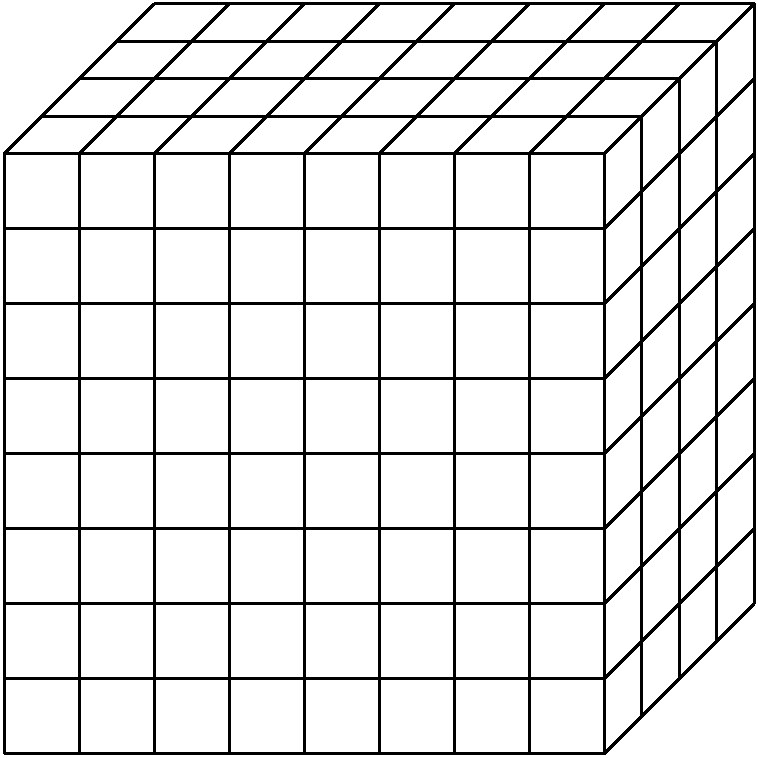
\includegraphics[width=0.5\textwidth]{MunWal00lattice}
  \caption{
3\dmn\ lattice. From \refref{MunWal00}.
  }\label{fig:MunWal00lattice}
\end{figure}
%%%%%%%%%%%%%%%%%%%%%%%%%%%%%%%%%%%%%%%%%%%%%%%%%

In Euclidean field theory the fields $\field(x)$ depend on the $d$ Euclidean
coordinates, so introduce a discretized spacetime in form of a
$d$-periodic hypercubic \emph{integer lattice} $\integers^d/\speriod{}^d$
(see \reffig{fig:MunWal00lattice}), with lattice spacing $a_{i}=\Delta
x_{i}$ and lattice period $\speriod{i}=1/\Delta x_{i}$ along the unit
vector
\[
\hat{n}_{i}
    \in
\left\{\hat{n}_1, \hat{n}_2, \cdots , \hat{n}_d\right\}
\]
pointing in the $i$th positive direction. The (scalar) \emph{field}
$\field(x)$ is evaluated only on the lattice points
\beq
\field_z
=
\field(x)
    \,,\qquad \qquad x = az= \mbox{lattice point}
    \,,\quad z \in \integers^d/\speriod{}^d
\,.
\ee{LattField}
It is periodic
\[
\field_z = \field_{z+\speriod{i}\hat{n}_{i}}.
\]
in all directions.
We refer to the set of values of $\Xx=\{\field_z\}$ as a {\em {\lattstate}}.
    \index{lattice!state}\index{lattice!configuration}

In order to discretize field-theoretic partial differential equations, we
need to {lattice derivatives}.
The  {\em forward partial lattice derivative}
    \index{lattice!derivative}\index{derivative, lattice}
    \index{lattice!derivative, forward}
\beq
(\partial_{i} \field)_z
        =
    \frac{\field(x+\Delta x_{i}{\hat{n}_{i}}) - \field(x)}{\Delta x_{i}}
        =
    \frac{\field_{z+{\hat{n}_{i}}} - \field_z}{\Delta x_{i}}
%\,.
\ee{latticePartDer}
depends explicitly on the lattice spacing. For our purposes it is
convenient to reformulate the problem as a discretization on
an integer lattice.
This is attained by converting all continuum partial \emph{derivatives}
into discrete partial \emph{differences} by
\(
\partial_{i} \to \speriod{i}\partial_{i}
\)
rescaling of the partial derivatives. After this rescaling $\partial_{i}$
is an integer lattice forward partial {\em difference operator}
\beq
\partial_{i} = \shift_{i}  - \unit
\,.
\ee{forwDer}
Higher lattice partial difference operators can be defined as\rf{Elaydi05}
\beq
\pde_{i}^k = \sum_{j=0}^k(-1)^j\,\combinatorial{k}{j}\,\shift_{i}^{k-j}
\,,
\label{Elaydi05(2.1.1)}
\eeq
with support on $k+1$ forward points. For example
\bea
\partial_{i}^2 &=& \shift_{i}^2  - 2\shift_{i} + \unit
            \continue
\partial_{i}^3 &=& \shift_{i}^3  - 3\shift_{i}^2  + 3\shift_{i} - \unit
\,.
\label{Elaydi05(2.1.1a)}
\eea
The even ones can be centered to be
reflection symmetric (symmetric under transposition) by translation by
$k$ sites,
\bea
\Laplacian_{i} &=&  - \transp{\partial}_{i}\partial_{i}
        \,=\, \shift_{i}  - 2\unit + \shift_{i}^{-1}
            \continue
\Laplacian_{i}^2 &=& \shift_{i}^2 - 4\shift_{i} + 6\unit  - 4\shift_{i}^{-1} + 6\shift_{i}^{-2}
\,,
\label{Box(2.1.1)}
\eea
where $\Laplacian=\sum\Laplacian_{i}$ stands for the lattice Laplacian
(or d'Alambertian).

Spacetime integrals are now replaced by sums,
\[
\int\!d^dx \quad \longrightarrow  \sum_x a^d
\,,
\]
    \PC{2020-03-15}{
\[
\partial_{\mu}\ssp(x) =
\frac{1}{a} (\ssp(x+a{\hat{\mu}})-\ssp(x)),
\]
and spacetime integrals by sums:
\[
\int\!d^4x \quad \longrightarrow  \sum_x a^4 \ .
\]
    }
and the lattice free field action is
\bea
S &=&
\sum_x a^d \left\{ \frac{1}{2} \sum_{i =1}^d
(\partial_{\mu}\field(x))^2 + \frac{m^2}{2}\field(x)^2
% + \frac{g_0}{4!}\field(x)^4
\right\}
\continue
 &=&
\sum_z a^d \left\{\frac{1}{2}\sum_{i =1}^d
\field_z\left(-\Laplacian_{i} + m^2\right)_{zz'}\field_{z'}
\right\}
\,.
\label{MunWal00freeAct}
\eea
In the functional integrals the measure
\[
{\cal D}\field  =  \prod_x d\field(x)
\]
involves the lattice points $x$ only, so for a finite lattice this is a
finite dimensional integral.

involves the lattice points $x$ only, so we have a discrete set
of variables to integrate. If the lattice is taken to be finite, we just
have finite dimensional integrals.

    \PC{2020-03-15}{
Let us assume a hypercubic lattice with length $L_1=L_2=L_3=L$ in
every spatial direction and length $L_4=T$ in Euclidean time,
\[
x_{\mu} = an_{\mu},\qquad n_{\mu} = 0,1,2,\dots,L_{\mu}-1,
\]
with finite volume $V = L^3T$, and periodic boundary conditions
\[
\ssp(x) = \ssp(x+aL_{\mu}\,\hat{\mu}),
\]
where $\hat{\mu}$ is the unit vector in the $\mu$-direction.
    }

The momenta are also discretized,
\[
p_{\mu} = \frac{2\pi}{a}\,\frac{l_{\mu}}{\speriod{\mu}}\qquad \mbox{with}\
l_{\mu} = 0,1,2,\dots,\speriod{\mu}-1,
\]
and the momentum-space integration is replaced by finite sums
\[
\int\!\frac{d^4p}{(2\pi)^4}\ \longrightarrow \
\frac{1}{a^4 \speriod{}^3 T}\sum_{l_{\mu}}
\,.
\]
All ``functional integrals'' are now regularized, finite
expressions.

To recover physics in a continuous and infinite spacetime, one needs to
take the infinite volume limit,
\[
\speriod{},T \longrightarrow \infty
\,,
\]
and the continuum limit,
\[
a \longrightarrow  0.
\]
We shall not discuss the continuum limit of a lattice field theory here.

\subsection{Transfer matrix}
\label{sect:transfMat}

Picking out a `time direction' and evolving in time slices (what we call
Hamiltonian formulation) is here called `transfer matrix', presumably in
reference to the similar formulation for the Ising model.

Split the 4D hypecubic lattice $z=(z_1,z_2,z_3,z_4)$ into 3\dmn\
`spatial' directions $\textbf{z}=(z_1,z_2,z_3)$ and the `temporal'
direction $z_4=\zeit$.
Let
\beq
\Xx_\zeit = \{\field_z | z_4=\zeit\}
\ee{MonMun94:(1.184)}
be a  field configuration on a Euclidean time slice $z_4=\zeit$.
Decompose the lattice action as
\beq
S[\field] = \sum_\zeit L[\Xx_{\zeit+1},\Xx_\zeit]
\ee{MonMun94:(1.185)}
This sum looks like the usual 1D temporal lattice action \refeq{MacMei83-4}.
Here
\beq
L[\Xx_{\zeit+1},\Xx_\zeit]=
          \sum_{\textbf{z}}\frac{1}{2}(  \field_{\textbf{z},\zeit+1}
                                        -\field_{\textbf{z}\zeit}   )^2
        + \frac{1}{2}(L_1[\Xx_\zeit] + L_1[\Xx_{\zeit+1}])
\ee{MonMun94:(1.186)}
with (here I drop a non-harmonic potential terms)
\beq
L_1[\Xx_\zeit]=
          \sum_{\textbf{z}}\frac{1}{2}
           \left\{\sum_{k=1}^3(\field_{\textbf{z}+\hat{k},\zeit}
                               -\field_{\textbf{z}\zeit})^2
                                + \frac{m^2}{2}\field_{\textbf{z}\zeit}^2
           \right\}
\ee{MonMun94:(1.187)}
Eq.~\refeq{MonMun94:(1.186)} looks like a sensible generalization of the
temporal lattice generating function \refeq{MKMP84(3.6)}.

The transfer matrix is defined as
\beq
T[\Xx_{\zeit+1},\Xx_\zeit]=
        e^{-L[\Xx_{\zeit+1},\Xx_\zeit]}
\ee{MonMun94:(1.188)}
As the matrices are presumably not commuting,
it is not obvious to me that repeated application of the
transfer operator adds up to the lattice action $S[\field]$
\refeq{MonMun94:(1.185)} in the exponent.
Take a field $\Psi_\zeit$ defined on $\zeit$ time-slice. Then the
transfer operator evolves the initial time-slice by matrix multiplication,
\beq
T^\cl{}\Psi_\zeit=\Psi_{\zeit+\cl{}}
\ee{MonMun94:(1.189)}
As it stands, it is not obvious how this is supposed to work, but Montvay
and M{\"u}nster\rf{MonMun94} do give the standard differential
formulation, explain correlations, \etc, so it's probably OK. For a
time-periodic lattice of time period $\period{}$ they say that
\beq
Z= \Tr T^\cl{}
\ee{MonMun94:(1.196)}
is the \emph{partition function}.

\begin{description}
  \item[2020-07-04 Predrag]
Would be happier if \refeq{MonMun94:(1.196)} were a $\Det$,
\ie, if there were a
\(
T=1-zJ
\)
kind of expression. But ...
I do not see a quick way from here to the Hill's formula, so I abandon
this path for now.
\end{description}

\subsection{Classical {$\phi^3$} lattice field theory}
\label{sect:phi3latt}

\begin{description}
  \item[2021-12-23 Predrag]
All {$\phi^k$} lattice field theories fit under the ``generalized
\HenonMap'' umbrella, so {$\phi^3$}, {$\phi^k, k>4$} are covered in
\refsect{sect:HamHenonMap}~{\em {\Henlatt}; anti-integrable limit}

\end{description}

\subsection{Classical {$\phi^4$} lattice field theory}
\label{sect:phi4latt}

Field theorists do not like odd potentials, such as the {\henlatt}
\refeq{henlattBWcubic}, as they are not bounded from below.

We should be able to write \refeq{phi4actionSch} action
$S[\Xx]$ such that the derivative of the quartic term yields classical
{$\phi^4$} theory \refeq{KarZar12(69)} on $d$\dmn\ lattice
\beq
-\ssp_{\zeit+1} + \frac{g}{3!}\ssp_{\zeit}^3 - \ssp_{\zeit-1} = \Ssym{\zeit}
\,.
\label{phi4-1dLatt}
\eeq
To get some intuition, find the 3 steady states $\ssp_{\zeit}=\ssp$
by plotting
\beq
V'[\ssp] = 2\ssp  - \frac{g}{3!}\ssp^3 = 2\,\ssp(1 - \frac{g}{12}\ssp^2)
%\,,
\ee{phi4pot-1dLatt}
as a function of (sufficiently strong) stretching $g$, and then picking a
sensible constant source $\Ssym{\zeit}=\Ssym{}$ value
(or 3 values $\Ssym{\zeit}\in\{L,C,R\}$, see \refexam{exam:ReflectA}~{\em
A reflection--symmetric  $1d$ map.})
for which not only the 3 fixed points  are real, but all $3^\cl{}$
3-symbol bimodal map itineraries are realized.

Continued around \refeq{phi4antiInteg}.

\bigskip

The \HillDet\ $\|\jMorb[\Xx]\|$ is again of the same form
\refeq{jMorb1dField}, with the stretching factor at site $\zeit$
depending on the coupling constant ${g}$, the lattice site field for the
given \lattstate.

For example, the {\HillDet} of the $[4\times4]$ \jacobianOrb\ $\jMorb$ is
({\color{red}correct this!}):
\bea
\Det(\jMorb)
&=&
\left\|
\begin{array}{cccc}
 {s}_1 &-1 & 0 &-1  \\
-1 & {s}_2 &-1 & 0 \\
 0 &-1 & {s}_3 &-1 \\
-1 & 0 &-1 & {s}_4
\end{array}
\right\|
     \label{HillDet4x4}\\   % was {LC21:HLdetCycD8s1}
&=&
  {s}_1 {s}_2 {s}_3 {s}_4 +{s}_1 {s}_2 {s}_3
+ {s}_2 {s}_3 {s}_4
\ceq
 +{s}_1 {s}_2
 +{s}_2 {s}_3
 +{s}_1 {s}_4
 +{s}_3 {s}_4 +{s}_1 +{s}_2 +{s}_3 +{s}_4
   \,.
\nnu
\eea

\begin{description}


\PCpost{2016-08-20}{
Might be worth a look - several papers on coupled map lattices, see
also \refref{HooAok16} on order and chaos in a continuous time,
1\dmn\ latticel $\phi^4$
model - if you read that literature, please share what you have learned
by writing it up there.
    }

\item[2021-08-11 Predrag]

Karimipour and Zarei\rf{KarZar12}
{\em Completeness of classical {$\phi^4$} theory on two-dimensional lattices}
\arXiv{1201.4558}:

The 2\dmn\ $\phi^4$ Hamiltonian for all discrete scalar field theories on
a two dimensional square lattice with periodic boundary conditions
\beq
  H_c=
  \sum_{\langle r,s\rangle}K_{r,s}(\phi_r-\phi_s)^2
  +\sum_{r}h_r \phi_r +m_r \phi_r^2+ q_r \phi_r^4,
\ee{KarZar12(69)}
where $K_{r,s}\in \{i,-i\}, \ i=\sqrt{-1}$ and the real
parameters $h_r$, $m_r$ and $q_r$ denote respectively the
inhomogeneous external field, the quadratic (mass term) and
quartic coupling strengths. The linear terms $\{h_r\}$ are also
necessary for completeness.

From
\HREF{http://www.scholarpedia.org/article/Triviality_of_four_dimensional_phi\%5E4_theory_on_the_lattice}
{Scholarpedia}:
action
\beq
S = \sum_z \left[ \varphi_z^2 + \lambda \left( \varphi_z^2 - 1 \right)^2 \right]
    - 2 \kappa \sum_{\langle z z' \rangle} \varphi_z \varphi_{z'}
\,.
\ee{phi4actionSch}


\item[2021-12-05 Predrag]
$\phi^4$ theory also shows up in Br{\'e}zin \& Zinn-Justin
(see \refsect{sect:MFT-Ising}) {\em Mean field theory for the Ising model}.
Their formulation suggests that the partition function \refeq{partFunct} should be
written as \refeq{NKHM15cw} where $f[\Xx]$ is free energy (the
large-deviation potential)
\beq
Z[\source]	= e^{-{N_\lattice} f[\source]}
\,.
\ee{NKHM15ZJ}
and $N_\lattice$ is the number of lattice sites.

\item[2021-12-07 Predrag]

Vierhaus's masters thesis\rf{Vierhaus10} {\em Simulation of {$\phi^4$}
theory in the strong coupling expansion beyond the {Ising} Limit}
has a clear discussion of the
\HREF{https://edoc.hu-berlin.de/bitstream/handle/18452/14790/vierhaus.pdf?sequence=1&isAllowed=y\#section.2.3}
{Ising limit of {$\phi^4$}}.
Note the reformulation \refeq{phi4actionSch} of the action, his eq.~(2.15).

\item[2021-12-21 Predrag]
Hagiwara and Shudo\rf{HaShu04a}
{\em An algorithm to prune the area-preserving {H{\'e}non} map}
(2004)
describes Sterlings anti-integrable method.

Starting with the \henlatt\ second-order difference equation
\refeq{Hen-1dLattA}, changing
variables to $z = \epsilon x$, $\epsilon = a^{-1/2}$ gives
\beq
-\epsilon(z_{\zeit-1}+z_{\zeit+1}) + z_\zeit^2 - 1 = 0
\,.
\ee{HaShu04a(2)}
At the anti-integrable limit $\epsilon\to0$, the map
reduces to $z_\zeit^2 = 1$,
with every orbit an arbitrary sequence of $\pm1$.

\item[2021-12-22 Predrag] An unchecked reverse engineering guess:
Starting with the second-order difference equation for
$\phi^4$ theory:
\beq
-\epsilon(z_{\zeit-1}+z_{\zeit+1}) + z_\zeit(z_\zeit-1)(z_\zeit+1) = 0
\,.
\ee{phi4antiInteg}
At the anti-integrable limit $\epsilon\to0$, the map
reduces to $z_\zeit(z_\zeit-1)(z_\zeit+1)= 0$,
with every orbit an arbitrary sequence of $\{-1,0,1\}$.
Then go back to \refeq{phi4-1dLatt}, using
$\ssp= z/\epsilon$, $\epsilon = g^{-1/3}$.
\beq
- \ssp_{j-1} + g\,\ssp^3_j - \ssp_{j+1} =  g^{2/3}\ssp_j
\,.
\ee{PCphi4}
Probably not the right thing; note that
\refeq{Anastassiou21(6)} scales the linear term differently,
 by $\epsilon$.

\item[2021-12-22 Predrag]
Anastassiou, Bountis and B{\"a}cker\rf{AnBoBa17} {\em Homoclinic points of
{2D} and {4D} maps via the parametrization method} (2017):

the dynamics of discrete breather solutions on
1--dimensional
lattices (or chains) of nonlinearly interacting particles

The discrete nonlinear Klein-Gordon
system of ordinary differential equations
\beq
\ddot u_n=-V^\prime\left(u_n\right)+\alpha\left(u_{n+1}-2u_n+u_{n-1}\right)
\,, \quad
V(x)=\frac{1}{2}Kx^2+\frac{1}{4}x^4
\,,
\ee{AnBoBa17eq4}
where $u_n$ for $-\infty<n<\infty$ is the amplitude of the $n$-th
particle, $\alpha>0$ is a parameter indicating the strength of coupling
between nearest neighbors, and $V(x)$ is the on-site potential with
primes denoting differentiation with respect to the argument of $V(x)$.

Discrete nonlinear Schr{\"o}dinger equation is similar.


\item[2021-12-22 Predrag]
Must study Anastassiou\rf{Anastassiou21}
{\em Complicated behavior in cubic {H{\'{e}}non} maps},
(2021).
He defines the generalized \HenonMap\ of the plane onto itself as
\beq
H\colon \mathbb{R} ^2\to \mathbb{R} ^2,\qquad H(x,y)=(y, b\,x+p(y)),
\ee{Anastassiou21(3)}
The determinant of the Jacobian matrix connected to the dissipation of
the system is equal to $-b$. If the polynomial p(y) is odd, then the
map $H(x,y)$ is symmetric under the transformation
\beq
\sigma(x,y)=(-x,-y)
\,.
\ee{Anastassiou21(3a)}
For $-b=1$, the map is a symplectomorphism (or symplectic map)
because it preserves the natural symplectic form of the plane,
$dx\wedge{dy}$.

The dynamics of $H(x,y)$, where p(y) is a third-degree polynomial, was
studied in \refref{DulMei00}, sufficient conditions for hyperbolicity in
generalized {\HenonMap}s for arbitrary polynomials p(y) were given in
\refref{Zhang10}. Anastassiou studies cubic polynomial $p(y)$
{\HenonMap}s,
\beq
H\colon \mathbb{R} ^2\to \mathbb{R} ^2,\qquad H(x,y)
=\bigl(y,-b\,x+ g(y^3-y)\bigr),
\ee{Anastassiou21(4)}
studied from a different perspective in his earlier
articles\rf{AnBoBa17,AnBoBa18}. He locates the region of the \statesp\
\beq
\mathcal{A} =
\biggl\{(x,y)\in \mathbb{R} ^2\colon\,
 |x|,|y|\le \sqrt{1+\frac{2}{g}}\,\biggr\}
\,,
\ee{Anastassiou21(4a)}
where the bounded  nonwandering invariant set exists, and finds parameter
values \(g>4\) for which this nonwandering set is hyperbolic. Read his
proof - it is instructive.
% For this, he uses a classical result of Afraimovich et al.[13].
Remember that these are just very crude bounds - the stable/unstable
manifolds will give tight bounds.
He shows that his map is conjugate to the Bernoulli three-shift, using
the anti-integrability technique\rf{aub95ant,Chen04,BolMac97,BaChMa13}.
\[
-\ssp_{n+1} + g\,\ssp_{n}^3  -g\,\ssp_{n} - \ssp_{n-1}=0
\,,
\]
Define $\epsilon =1/g$
\beq
- \epsilon(\ssp_{n+2} + \ssp_{n+1}) + \ssp_{n+1}^3=\epsilon \,\ssp_n
\,,
\ee{Anastassiou21(6)}

It is customary to say that such a complex behavior is `chaotic' because
of Devaney's definition\rf{BBCDS92}.

\item[2021-06-04 Predrag]
Friedland and Milnor\rf{FriMil89}
{\em Dynamical properties of plane polynomial automorphisms} (1989)
introduced the generalized \HenonMap. Their theorem 2.6 on the normal
form of such maps is nice. In their fig.~2 they do the 0th order version
of the plot I hope Harrison and Ibrahim will plot: the three-fold
horseshoe associated with a real cubic polynomial.
Dullin and Meiss\rf{DulMei00} do that, their fig.~13\,(right).

\item[2021-06-04 Predrag]
See also Anastassiou, Bountis and B{\"a}cker\rf{AnBoBa18} (2018)
{\em {Recent results on the dynamics of higher-dimensional {H{\'{e}}non} maps}},
their fig.~1. They take
\beq
p(y) = cy + 3y^3
\ee{AnBoBa17}
They chose $c=-\frac{5}{2}$ throughout their publication (we should too,
to compare results).
``This choice is pictorially convenient, since $c$ values in that range
produce large scale manifolds that are clearly visible in the figures.''

The cubic mapping possesses three fixed points: saddle point at the
origin, for all parameter values, a symmetric pair at
\[
\left(\pm\sqrt{(2-c)/3},\pm\sqrt{(2-c)/3}\right)
\,.
\]
The $(0,0)$ fixed point Floquet multipliers are
\begin{equation}
   \frac{1}{2}\left(c-\sqrt{c^2-4}\right),
   \frac{1}{2}\left(c+\sqrt{c^2-4}\right)
   \,.
\end{equation}
Since $c=-5/2$ and $\delta=1$, the Floquet multipliers of the origin are
$\ExpaEig_u = -2$ and $\ExpaEig_s = -1/2$
with normalized eigenvectors
$(-1/\sqrt{5}, 2/\sqrt{5})$ and $(-2/\sqrt{5}, 1/\sqrt{5})$.
The origin is thus a saddle, with a 1--dimensional stable and a 1--dimensional
unstable manifold, whose parametric computation they explain.

\item[2021-06-04 Predrag]
Dullin and Meiss\rf{DulMei00}
{\em Generalized {H{\'{e}}non} maps: the cubic diffeomorphisms of the plane}
(2000):

 The Euler–Lagrange equation associated with this action is
\beq
 m(\ssp_{\zeit-1}+ \ssp_{\zeit+1}) =U'(\ssp_{\zeit})
\ee{DulMei00(20)}
which is the Lagrangian form of the \HenonMap.
They concentrate on the area-preserving cubic maps. [...]
These are reversible and have an additional symmetry on a codimension-one
line in parameter space (Predrag currently calls that `dynamical symmetry').

\item[2021-06-04 Predrag]
The Arneodo–Coullet–Tresser maps (referred to in \rf{LiMal04}) are
5-term recurrence equations with $\ssp_\zeit^k$ nonlinear term, ignore for now.

Li and Malkin\rf{LiMal04}
   {\em Bounded nonwandering sets for polynomial mappings} (2004)


\end{description}


%\newpage
\section{Normalizing flows}
\label{sect:discFTblog}

\textbf{Predrag}: What is here called

   `normalizing flow' \(f: \mathcal{X} \rightarrow \mathcal{X}\),
  invertible and differentiable

  Jacobian factor \(J(z) = |\det \partial f_i(z) / \partial z_j|\)

\noindent
is the main
idea of our \refrefs{conjug_Fred,CFTsketch}); what they call their
`latent' space probability distribution being set to Gaussian is what we
call `free field theory'. One pays a determinant of the Jacobian matrix
of that field transformation, the same as for us. But Miranda Cheng says
that this determinant ``can be easily computed/approximated" which is
news to me.

\begin{description}


\item[2021-11-01 Predrag]
 Miranda Cheng \\
\videoLink{YouTube.com/embed/%
Ff_jllXzMfk}
{\em Machine learning and theoretical physics: some applications}.

Lattice field theory is the main tool for doing nonpertubative
calculations in field theory.
The idea of ML techniques, such as Normalizing Flows, is that if we can
learn an invertible map that trivializes an interacting model to a free
theory, we can easily sample the latter and push back the samples through
the inverse map to obtain (proposed) samples from the original
non-trivial distribution.

\textbf{Predrag}: this is the main idea of our \refref{conjug_Fred,CFTsketch});
what they call their `latent' space probability distribution being set to
Gaussian is what we call `free field theory'. One pays a determinant of the
Jacobian matrix of that field transformation, the same as for us. But she says
that this determinant ``can be easily computed/approximated" which is news to me.

In the talk she defines the ``observable'' the way we would; I have not
seen the definition yet in their papers.

The first part is based on

Pim de Haan, Corrado Rainone, Miranda Cheng and  Roberto Bondesan%\rf{dRCB21}
{\em Scaling Up Machine Learning For Quantum Field Theory with
Equivariant Continuous Flows}, \arXiv{2110.02673}.
Cheng has typos in her presentation (probability density
$"+"\Det|J|$ rather than $\times$).

the contributions of their paper:
\vspace{-7pt}
\begin{itemize}
    \item They extend %\cite{pmlr-v119-kohler20a}
    and develop continuous normalizing flows for lattice field theories
    that are fully equivariant under lattice symmetries as well as the
    internal $\phi \mapsto -\phi$ symmetry of the $\phi^4$ model.
    \item They train our model for the $\phi^4$ theory and and for the
    $32\times 32$ lattice we improve the effective sample size from 1\%
    to 66\% w.r.t.~a real NVP baseline of similar size.
    % 5(Fig.~\ref{fig:results}).
    \item They study equivariance violations of real NVP models and
    contrast it with the exact equivariance of our flows.
\end{itemize}


If the vector field $g$ is equivariant, the resulting distribution on
$\phi$ is invariant. They show how to construct a $g$ equivariant to the
square lattice symmetries.

\paragraph{The $\phi^4$ theory}
possesses non-trivial symmetry properties and a phase
transition. In the case of $\phi^4$ theory in two dimensions, the {\em
field configuration} is a real function on

the vertex set $V_L$ of the square lattice

with periodic boundaries and size $L\times L$: $\phi: V_L \to
{\mathbb R}$.
The $\phi^4$ theory is described by a probability density
\beq
p(\phi) = \exp(-S(\phi))/Z
\,,
\ee{dRCB21probField}
with action
\beq
S(\phi) = \sum_{x,y\in V_L}\phi(x) \Delta_{x,y} \phi(y) + \sum_{x\in V_L}m^2\phi(x)^2 + \mathit{\lambda}\phi(x)^4
\label{dRCB21eq:S}
\eeq
Here $\Delta$ is Laplacian matrix of the square lattice $({\mathbb
Z}/L{\mathbb Z})^{\times 2}$, $m$ and $\lambda$ are numerical parameters.
In the case of this and other non-trivial field theoretical densities,
%direct sampling is impossible due to the statistical correlation between
%degrees of freedom spatially separated up to the \emph{correlation
%length} of the theory, a fundamental quantity denoted as $\xi$;
$Z$ is the normalisation factor that is not known analytically for $\lambda\neq 0$.

  Probability densities over those \statesp\ manifolds:

  \begin{itemize}
  \item
    Prior density \(r(z)\)
  \item
    Model density \(q(x)\)
  \item
    Target density \(p(x)\)
  \end{itemize}




Note that, besides the space-time symmetries of the periodic lattice,
the theory possesses a

discrete global symmetry $\phi \mapsto -\phi$.

We
shall choose the couplings in such a way that only one minimum of the
action, invariant under this symmetry, exists. See
[??] %\cite{hackett2021flowbased}
for relevant work in the case of a symmetry-broken case.

(Was commented out:)
We will work in the ``unbroken" phase with $m^2>0$,
%\MC{actually, $m^2$ is negative as we report in the table},
where the minimum of the action is
invariant under the global symmetry.
See \arXiv{2107.00734} for relevant work in the broken phase.

The periodic lattice $V_L$ has spatial symmetry group $G=C_L^2 \rtimes
D_4$, the semi-direct product of two cyclic groups $C_L$ of translations
and dihedral group $D_4$ of right angle rotations and mirrors.
To ensure spatial equivariance of the vector field model, we should have
that

$\forall g \in G, x,y,a, f, W_{g(x)g(y)af}=W_{xyaf}$.

Using the translation subgroup, we can map any point $x$ to a fixed point
$x_0$. This allows us to write $W_{xyaf}=W_{x_0t_x(y)af}$, $t_x(y) = y -
x + x_0$.

(Predrag - they seem to be defining the point group here:)\\
Then let $H\simeq D_4$ be the subgroup of $G$ such that $g(x_0)=x_0$ for
all $g\in G$, and denote the orbit of $y$ under $H$ by $[y]=\{y' \mid
\exists g \in H, g(y)=y'\}$.

For each such orbit $[y]$ and dimension $a$
and $f$, a free parameter $W_{[y]af}$ exists, so that the other
parameters are generated by $W_{xyaf}=W_{[t_x(y)]af}$.


(Was commented out; Predrag - they ignore symmetric lattice states here:)\\
As most orbits are of size 8, the number of free parameters per $a$ and
$f$ is approximately $L^2/8$.

The orbits of $D_4$, leaving point $(0, 0)$ invariant, for $L=16$ are
shown in Fig.~4. %\ref{fig:orbits} in the Appendix
For each color in that figure, for each
dimensions $a$ and $f$, we have a free parameter.\\
(Predrag - that figure says the 1/8th fundamental domain tiles
the square lattice, and ignores the symmetry boundaries. The ``free parameter''
is just the values of the field in the fundamental domain.)


\item[2021-12-05 Predrag]
These papers seem to be more informative:

Rezende and Mohamed  (2015) ``normalizing flows''
\arXiv{1505.05770}
\\
cites   Jordan,  Ghahramani,  Jaakkola  and Saul\rf{JGJS99}
{\em An introduction to variational methods for graphical models} (1999)

Del Debbio, Rossney and Wilson {\em Efficient Modelling of Trivializing
Maps for Lattice $\phi^4$ Theory Using Normalizing Flows: A First Look at
Scalability} \arXiv{2105.12481}

\item[2021-12-05 Predrag]
%@misc{albergo2021introduction,
Albergo, Boyda, Hackett, Kanwar, Cranmer, Racanière,
Jimenez Rezende and Shanahan, %\rf{ABHKCRJS21}
{\em Introduction to Normalizing Flows for Lattice Field Theory}
(2021),
\arXiv{2101.08176}:

      This notebook tutorial demonstrates a method for sampling Boltzmann
      distributions of lattice field theories using a class of machine
      learning models known as normalizing flows. The ideas and
      approaches proposed in

\arXiv{1904.12072}

\arXiv{2002.02428}

\arXiv{2003.06413}

      are reviewed and a concrete implementation of the
      framework is presented. We apply this framework to a lattice scalar
      field theory and to U(1) gauge theory, explicitly encoding gauge
      symmetries in the flow-based approach to the latter.

%@article{PhysRevLett.125.121601,
%  title = {Equivariant Flow-Based Sampling for Lattice Gauge Theory},
%  author = {Kanwar, Gurtej and Albergo, Michael S. and Boyda, Denis and Cranmer, Kyle and Hackett, Daniel C. and Racani\`ere, S\'ebastien and Rezende, Danilo Jimenez and Shanahan, Phiala E.},
%  journal = {Phys. Rev. Lett.},
%  volume = {125},
%  pages = {121601},
%  year = {2020},
%  doi = {10.1103/PhysRevLett.125.121601},
%}

The Box-Muller transform is an example of a `normalizing' transformation:
to produce Gaussian random variables, draw two variables \(U_1\) and
\(U_2\) from \(\text{unif}(0,1)\), then change variables to
\beq
    (Z_1,Z_2) = (r\,\cos(2\pi U_2),\,r\,\sin(2\pi U_2))
\,,\qquad r= \sqrt{-2 \ln{U_1}}
\,.
\ee{ABHKCRJS21(1)}
The resulting variables \(Z_1, Z_2\) are then distributed according to
an uncorrelated, unit-variance Gaussian distribution; $U_1$ controls the
radius, and $U_2$ the angle of a $2d$ Gaussian.
\\
{\bf Predrag}: {\color{red}
This might relate Bernoulli and \templatt\ to Gaussian field theories
(see \refsect{sect:GaussianModel}), \ie, this maps fields in $[0,1)$
to fields in $\reals$.
                }

The density associated with output samples is computed
by the \emph{change-of-variables formula} relating the \emph{prior
density} \(\rho(U_1, U_2) = 1\) to the \emph{output density}
% \(q(Z_1, Z_2)\):
\beq
\begin{split}
    q(Z_1, Z_2) &= \rho(U_1, U_2) \left|
    \det\frac{\partial Z_k(U_1, U_2)}{\partial U_l} \right|^{-1} \\
    &= 1 \times \left| \det \left( \begin{matrix}
        \frac{-1}{U_1 r} \cos(2\pi U_2) &
        - 2\pi r \sin(2\pi U_2) \\
        \frac{-1}{U_1 r} \sin(2\pi U_2) &
        2\pi r \cos(2\pi U_2)
        \end{matrix} \right) \right|^{-1} \\
    &= \left| \frac{2 \pi}{U_1} \right|^{-1}.
\end{split}
\ee{ABHKCRJS21(2)}
\(J(U_1,U_2)\equiv\det({\partial Z}/{\partial U})\)
is the determinant of the Jacobian
of the coordinates transformation \((U_1,U_2)\to(Z_1,Z_2)\). The Jacobian
factor is a change in volume element, therefore the change-of-variables
formula must contain the inverse of this factor (spreading out volume
decreases density). As
\[U_1 = \exp(-(Z_1^2 + Z_2^2) / 2)\] and the initial density $\rho(U_1,U_2)$
over the unit square was uniform, the transformed density is
\beq
    q(Z_1, Z_2) = \frac{1}{2\pi} e^{-(Z_1^2 + Z_2^2)/2}
\,.
\ee{ABHKCRJS21(3)}
This example has no free parameters because no extra parameters were needed
to create a transform that exactly reproduced the desired target
distribution, independent, unit-variance Gaussian. In general, we may not
know a normalizing flow that exactly produces our desired distribution,
and so instead construct parametrized models that we can variationally
optimize to \emph{approximate} that target distribution, and because we
can compute the density these can be corrected to nevertheless guarantee
exactness.

In some cases, it is easy to compute the Jacobian factor even when the
whole Jacobian matrix is intractable; for example, only the diagonal
elements are needed if the Jacobian matrix is known to be triangular.

The hypercubic lattice discretization of the derivatives of the continuum
Euclidean action gives rise to a lattice Euclidean action,
\beq
\begin{split}
S^E_{\text{cont}}[\phi] &=
\int d^2\vec{x} ~ (\partial_\mu \phi(\vec{x}))^2 + m^2 \phi(\vec{x})^2
                  + \lambda \phi(\vec{x})^4
\\
\rightarrow
S(\phi) &= \sum_{\vec{n}} \phi(\vec{n})
    \left[ \sum_{\mu \in \{1,2\}}
      - \phi(\vec{n}+\hat{\mu}) + 2\phi(\vec{n})  - \phi(\vec{n}-\hat{\mu})
    \right]
    + m^2 \phi(\vec{n})^2 + \lambda \phi(\vec{n})^4
\end{split}
\ee{ABHKCRJS21(11)}
where now \(\phi(\vec{n})\) is only defined on the sites
of the \(L_x \times L_y\) lattice, \(\vec{n} = (n_x, n_y)\), with
integer \(n_x, n_y\).
% We have implicitly moved to ``lattice units'' where \(a=1\) such that
% \(L_x, L_y, V\) are integers and all quantities are unitless.
The discretized field \(\phi\) can be thought of
as an \((L_x \times L_y)\)-dimensional vector. We use periodic boundary
conditions in all directions, i.e.~\(\phi(L_x, y) \equiv \phi(0, y)\),
etc.

More details on \(\phi^4\) lattice scalar field theory can be found in
%\cite{vierhaus2010simulation}.
%
% 2010-07-27 Diplomarbeit
Vierhaus's masters thesis\rf{Vierhaus10} {\em Simulation of {$\phi^4$}
theory in the strong coupling expansion beyond the {Ising} Limit}.
%\HREF{https://doi.org/10.18452/14138} {DOI: 10.18452/14138}.

  The lattice action then defines a probability distribution over
configurations \(\phi\), \begin{equation}
p(\phi) = \frac{1}{Z} e^{-S(\phi)}, \quad
Z \equiv \int \prod_{\vec{n}} d\phi(\vec{n}) ~ e^{-S(\phi)},
\end{equation} where \(\prod_{\vec{n}}\) runs over all lattice sites
\(\vec{n}\). This is the distribution we are training the normalizing
flows to reproduce. While \(Z\) is difficult to calculate, in practice
we only need \(p(\phi)\) up to a constant. The action can be efficiently
calculated on arbitrary configurations using Pytorch. Note that while
the theory describes 2D spacetime, the dimensionality of distribution
\(p(\phi)\) is the number of lattice sites, scaling with the volume of
the lattice.

  The theory has a symmetric phase and a broken symmetry phase,
corresponding respectively to nearly one mode of the distribution or two
widely separated modes (with intermediate configurations suppressed
exponentially in volume). The broken symmetry phase can be accessed for
\(m^2 < 0\) and \(\lambda\) less than a critical \(\lambda_c\). For
simplicity, we restrict focus to the \textbf{symmetric phase}, but
remain close to this phase transition such that the system has a
non-trivial correlation length.

A selection of references to related works (find the links in
\arXiv{2101.08176}):
\begin{itemize}
\item
  \textbf{Normalizing flows:}
  Agnelli \etal~(2010); %\cite{Agnelli2010ClusteringAC};
  Tabak and Vanden-Eijnden (2010); %\cite{tabak2010};
  Dinh \etal~(2014); %\cite{Dinh:2014};
  Dinh \etal~(2016); %\cite{dinh2016density};
  Papamakarios \etal\
    {\em Normalizing flows for probabilistic modeling and inference} (2019),
    \arXiv{1912.02762};
  % Papamakarios \etal~(2019)\cite{papamakarios2019normalizing}
\item
  \textbf{Symmetries and equivariance:}
  Cohen and Welling (2016); %\cite{cohen2016group};
  Cohen \etal~(2019); %\cite{cohen2019gauge};
  Rezende \etal~(2019); %\cite{rezende2019equivariant};
  K{\"o}hler \etal~(2020); %\cite{kohler2020equivariant};
  Luo \etal~(2020); %\cite{luo2020gauge};
  Favoni \etal~(2020); %\cite{favoni2020lattice}
\item
  \textbf{Flows on manifolds:}
  Gemici \etal~(2016); %\cite{gemici2016normalizing};
  Falorsi \etal~(2019); %\cite{falorsi19lie};
  Finzi \etal~(2020); %\cite{Finzi:2020};
  Mathieu and Nickel (2020); %\cite{mathieu2020riemannian};
  Falorsi and Forr{\'e} (2020); %\cite{falorsi2020neural}
\item
  \textbf{Applications of flows:} M{\"u}ller \etal~(2018)
; %\cite{mller2018neural};
  No{\'e} \etal~(2019); %\cite{noe2019boltzmann};
  Wu \etal~(2020); %\cite{wu2020stochastic};
  Dibak \etal~(2020); %\cite{dibak2020temperaturesteerable};
  Nicoli \etal~(2021) \HREF{https://doi.org/10.1103/PhysRevLett.126.032001} {DOI}
\end{itemize}

\item[2021-12-13 Predrag]
Sara liked very much this morning’s talk by
\HREF{https://staff.fnwi.uva.nl/m.welling/} {Max Welling} on ML for PDEs
– the way he controls the PDE grid, incorporates symmetries into the NN
part of the algorithm.

Garcia Satorras, Victor and Hoogeboom, Emiel and Fuchs, Fabian and
Posner, Ingmar and Welling, Max
\HREF{https://proceedings.neurips.cc/paper/2021/hash/21b5680d80f75a616096f2e791affac6-Abstract.html}
{{\em E(n) Equivariant Normalizing Flows}}
Advances in Neural Information Processing Systems 34 (2021):

This paper introduces a generative model equivariant to Euclidean
symmetries: E(n) Equivariant Normalizing Flows (E-NFs). To construct
E-NFs, we take the discriminative E (n) graph neural networks and
integrate them as a differential equation to obtain an invertible
equivariant function: a continuous-time normalizing flow. We demonstrate
that E-NFs considerably outperform baselines and existing methods from
the literature on particle systems such as DW4 and LJ13, and on molecules
from QM9 in terms of log-likelihood. To the best of our knowledge, this
is the first flow that jointly generates molecule features and positions
in 3D.





\end{description}




\newpage
\section{Noise is your friend}
\label{sect:noise}

\begin{description}
  \item[2021-11-27 Predrag]
Excerpts (mashed together in random order) from
Cvitanovi{\'c}, Dettmann, Mainieri and Vattay
  {\em Trace formulae for stochastic evolution operators}:
\\
{\em {Weak} noise perturbation theory}\rf{noisy_Fred} (1998),
\arXiv{chao-dyn/9807034},
and
\\
{\em {Smooth} conjugation method}\rf{conjug_Fred} (1998)
\arXiv{chao-dyn/9811003}.

These are the first two papers to treat time evolution
as a 1\dmn\ temporal lattice field theory.
They start out by
expressing the weak noise expansions in terms of Dirac $\delta$ and its
derivatives. In what is excerpted here we omit all correction terms, as we
are interested only into the leading behavior.
\end{description}

% predrag/articles/noise/noise.tex
%                   JStatPhys.tex is the submission version
% predrag/articles/noise/conjug/conjug.tex

The central object in the theory, the trace of the evolution operator,
is a discrete path integral, similar to those found in field theory
and statistical mechanics.

The theory is cast in the standard field
theoretic formalism, and weak noise perturbation theory written in terms of
Feynman diagrams.

The noise
tends to regularize the theory, replacing the deterministic delta function
evolution operators by smooth distributions.
While in this paper we are interested in effects of weak but
{\em finite} noise,
the $\sigma \to 0$ limit is also important as a tool for identifying
the natural measure\rf{sinai,bowen,ruelle} for deterministic flows.

We have cast the theory in the standard field theoretic
language\rf{FieldThe}, in the spirit of approaches such as the
Martin-Siggia-Rose\rf{MaSiRo73} formalism, the Parisi-Wu\rf{ParWu81}
stochastic quantization, and the
Feigenbaum and  Hasslacher\rf{FeHa82} study of noise renormalization
in period doubling.

The form of the perturbative expansions  % of \refsect{s:WeakNsPertExp}
is reminiscent of perturbative calculations
of field thery, but in some aspects the
calculations undertaken here are relatively more difficult.
The main difference is that there is
no translational invariance along the chain, so unlike the case of
usual field theory,
the propagator is not diagonalized by a Fourier transform. We
do our computations in configuration coordinates.
Unlike the most field-theoretic literature,
we are neither ``quantizing'' around a trivial vacuum,
nor a countable infinity of stable soliton saddles, but around an
infinity of nontrivial unstable hyperbolic saddles.

[...] our results are {\em a priori} far from obvious:
[...]
a more subtle and surprising result,
repeats of prime cycles can be resummed and theory reduced to the
\dzeta s and {spec\-tral det\-er\-min\-ant}s of the same form as the for the deterministic
systems.

[...] a discrete time 1-dimensional
discrete Langevin equation\rf{vKampen92,LM94},
\begin{equation}
x_{n+1}=f(x_n)+\sigma\xi_n
\,,\label{Langevin}
\end{equation}
with $\xi_n$ independent normalized
%Gaussian
random variables,
suffices to reveal the structure of the perturbative corrections.

We shall treat a chaotic system with such Gaussian weak external noise by
replacing the the deterministic evolution $\delta$-function kernel
by $\Lnoise{}$,  the Fokker-Planck
kernel corresponding to (\ref{Langevin}),
a sharply peaked noise distribution function
\beq
\Lnoise{} =\delta_\sigma(y-f(x))
\,,
\ee{Lnoise}
where  $\delta_\sigma$ is the Gaussian kernel
\beq
\delta_\sigma(z)=\frac{1}{\sqrt{2\pi\sigma^2}} e^{-z^2/2\sigma^2}
\,.
\ee{GaussKrnl}

In the weak noise limit the kernel is sharply peaked, so it
makes sense to expand it
in terms of the Dirac delta function and
its derivatives:
\beq
	\delta_\sigma(y)
	=
	\sum_{m=0}^{\infty} {a_m \sigma^m \over m!} \, \delta^{(m)}(y)
	=
	\delta(y) +
	a_2 {\sigma^2 \over 2} \delta^{(2)}(y) +
	% a_3 {\sigma^3 \over 6} \delta^{(3)}(y) +
    \dots
	\,.
\label{delSigExp}
\eeq
where
\[
	\delta^{(k)}(y) = {\pde^k \over \pde y^k} \delta(y)
	\,,
\]
and the coefficients $a_m$ depend on the choice of the kernel.
We have omitted the $\delta^{(1)}(y)$ term in the above because
in our applications we shall impose
the saddle-point condition, that is,
we shift $f$ by a constant to ensure that the noise peak corresponds
to $y=0$, so $\delta_\sigma^{'}(0)=0$.
For example, if $\delta_\sigma(y)$ is a Gaussian kernel,
it can be expanded as
\bea
	\delta_\sigma(y)
	&=&
	{1 \over \sqrt{2 \pi \sigma^2}} e^{-{y^2/2\sigma^2} }
%	=
%	\sum_{n=0}^{\infty}
%	\frac{\sigma^{2n}}{n!2^n} \delta^{(2n)}(y)
%	\continue	&=&
    =
	\delta(y) + {\sigma^2 \over 2} \delta^{(2)}(y)
	 % + {\sigma^4 \over 8} \delta^{(4)}(y)
     + \cdots
	\,.
\label{delGaussExp}
\eea

We start our computation of the weak noise corrections to the
spectrum of $\Lnoise{}$ by calculating the trace of the $n$th iterate of
the stochastic evolution operator $\Lnoise{}$
for a one-dimensional analytic
map $f(x)$ with additive noise $\sigma$.
This trace is an $n$-dimensional
integral on $n$ points along a discrete periodic chain,
so $x$ becomes an $n$-vector $x_a$ with indices $a,b,\ldots$
ranging from $0$ to $n$$-$$1$
in a cyclic fashion
\bea
\tr{\Lnoise{n}} &=& \int %dx_1 dx_2 ... dx_n \,
	\prod_{a=0}^{n-1} dx_a \, \delta_\sigma(y_a)
	\continue
y_a(x) &=& f(x_{a})  - x_{a+1}\,,\qquad x_n  =  x_0
\,.
\label{FatIntDef}
\eea

If the map is smooth, the periodic points of given finite
period $n$ are isolated and the noise broadening $\sigma$
sufficiently small so that they remain separated, the dominant
contributions come from neighborhoods of periodic points;
% \PC{state the crossover criterion}
in the
{\em saddlepoint approximation} the trace \refeq{FatIntDef} is given by
\beq
\tr{\Lnoise{n}} \longrightarrow \sum_{x_c\inFix{n}} e^{W_c}
\,,
\ee{SptSum}
As traces are cyclic,
$e^{W_c}$ is the same
for all periodic points in a given cycle, independent of the choice
of the starting point $x_c$.
Hence it is customary to rewrite this sum in terms of
prime cycles and their repeats,
\beq
\left. \tr{\Lnoise{n}} \right|_{\mbox{\footnotesize saddles}}
  = \sum_p \cl{p} \sum_{r=1}^\infty  e^{W_{p^r}}
\,,
\ee{SptSum1}
where $p^r$ labels the $r$th repeat of prime cycle $p$.

A fixed point and its repeats are of particular interest having the same
interaction at every site, as does the usual field theory. What we do
here is to formulate [...] the field theory on finite periodic
1-dimensional discrete chains.

Defining
$
y = f(x) -x
\,,
$
we can write the fixed point trace as
\beq
	\tr{\Lnoise{}}
	=
	\int dx\, \delta_\sigma(f(x)-x)
	= \int dy \, {1\over \left|y'(x)\right|}  \delta_\sigma(y)
	\,.
\label{(10)}
\eeq

We start by calculating the trace of the $n$th iterate of
the stochastic evolution operator $\Lnoise{}$
for a one-dimensional analytic
map $f(x)$ with additive Gaussian noise $\sigma$.
This trace is an $n$-dimensional
integral on $n$ points along a discrete periodic chain,
so $x$ becomes an $n$-vector $x_a$ with indices $a,b,\ldots$
ranging from $0$ to $n$$-$$1$
in a cyclic fashion
\bea
\tr{\Lnoise{n}} &=& \int[dx]\, \exp\left\{-\frac{1}{2\sigma^2}
\sum_{a}\left[x_{a+1}-f(x_a)\right]^2\right\}
	\continue
x_n  &=&  x_0 \,,\qquad [dx]=\prod_{a=0}^{n-1}{dx_a \over \sqrt{2\pi\sigma^2}}
\,.
\label{IntDef}
\eea
As we are dealing with a path integral on a finite discrete chain,
we find it convenient to rewrite the exponent in matrix notation
\beq
\tr{\Lnoise{n}} =\int[dx]\,
     e^{-\left[{\shift}^{-1}x -  f(x) \right]^2/2\sigma^2}
\,,\qquad
\shift_{ab}=\delta_{a,b+1}
\,,
\ee{eLnoisMtrx}
where $x$ and $f(x)$ are column vectors with components $x_a$ and $f(x_a)$
respectively,
and $\shift$ is the left cyclic shift or hopping matrix satisfying
$\shift^n=1$, ${\shift}^{-1}=\shift^{T}$.
Unless stated otherwise, we shall assume the repeated
index summation convention throughout, and that the
Kronecker $\delta$ function is the periodic one, defined by
\beq
\delta_{ab} = {1 \over n} \sum_{k=0}^{n-1} e^{i2\pi (a-b)k/n}
\,.
\ee{CycKronck}

[...]
if the noise is weak, the path integral \refeq{IntDef}
is dominated by periodic deterministic
trajectories.
Assuming that the periodic points of given finite period
$n$ are isolated and the trajectory broadening
$\sigma$
sufficiently small so that they remain clearly separated, the dominant
contributions come from neighborhoods of periodic points;
in the
{\em saddlepoint approximation} the trace \refeq{IntDef} is given by
\beq
\tr{\Lnoise{n}} \longrightarrow \sum_{x_c\inFix{n}} e^{W_c}
\,,
\ee{SdlptSum}
where the sum goes over all periodic points $x_c = x_{c+n}$ of period $n$,
$f^n(x_c)=x_c$. The contribution of the
$x_c$ neighborhood is obtained by
shifting the origin of integration to
\[
x_a \to x_a + \field_a
\,,
\]
where from now on $x_a$ refers to the position of the $a$-th periodic
point,
and expanding $f$ in Taylor series around each of the periodic points
in the orbit of $x_c$.

The contribution of the neighborhood
of the periodic point $x_c$ is given by
\bea
e^{W_c} &=& \int[d\field]\,
     e^{-\left(\InvPrpgtr{}\field_{} - V'(\field) \right)^2/2\sigma^2}
	\continue
%	 &=&  \int[d\varphi][d\overline{\psi}][d\psi]
%     e^{-\overline{\psi}\left(\InvPrpgtr{} -  V''(\field) \right)\psi
%		  -\varphi^2/2\sigma^2}
%		\continue
	&=& |\det \Prpgtr{}| \int[d\varphi]\,
     e^{\sum{1\over k} \tr\left(\Prpgtr{}V''(\field) \right)^k}
     e^{-\varphi^2/2\sigma^2}
\label{eWcMtrx}
\eea
where the propagator and interaction terms are collected in
\beq
\InvPrpgtr{}_{ab}\field_{b} = -\Df{}(x_{a})\field_{a}+\field_{a+1}
\,,\qquad
V(\field)= \sum_a \sum_{m=2}^{\infty}f^{(m)}(x_{a})
\frac{\field_{a}^{m+1}}{(m+1)!}
\,.
\ee{DefPrpg}
We find it convenient to also introduce a bidirectional propagator
$C=\Prpgtr{}\Prpgtr{}^T$ for reasons that will become apparent below.
In the second line of (\ref{eWcMtrx}) we have changed coordinates,
\beq
\varphi = \InvPrpgtr{}\field_{} - V'(\field)
\,,
\ee{eChaCoor}
and used the matrix identity $\ln\det M = \tr\ln M$ on the Jacobian
\beq
{1 \over \det \left(\InvPrpgtr{} - V''\right)}
 = {\det \Prpgtr{} \over
                    \det \left(1 - \Prpgtr{} V''\right)}
 = \det \Prpgtr{} \,
    e^{ -\tr \ln \left(1 - \Prpgtr{} V''\right) }
\,.
\ee{e:DetIdent}
The functional dependence
of $\field=\field(\varphi)$ is recovered by iterating (\ref{eChaCoor})
\beq
\field_a = \Prpgtr{}_{ab}\varphi_b + \Prpgtr{}_{ab}V_b'(\field)
\,.
\ee{eIterField}

The above manipulations are standard\rf{MaSiRo73} and often
used in the stochastic quantization literature\rf{ParWu81,DaHuRo90}.

As the sum is cyclic,
$e^{W_c}$ is the same
for all periodic points in a given cycle, independent of the choice
of the starting point $x_c$.
%
In the saddlepoint approximation we assume that the map is analytic
and the extrema $f^n$ are isolated.

From the second path integral representation in \refeq{eWcMtrx} it follows
that $\Prpgtr{}$ can be interpreted as the ``free'' propagator.
As $\Prpgtr{}$ will play a central role in what follows, we
write its inverse in its full [$n$$\times$$n$] matrix form:
\beq
\InvPrpgtr{}
	= {\shift}^{-1} - {\bf f'}
=%\pmatrix
\left(\begin{array}{ccccc}
  -\Df{0}         &  1    &        &        &      \cr
                  &-\Df{1}&  1     &        &      \cr
                  &       & -\Df{2}&  1     &      \cr
                  &       &        & \ddots &      \cr
             1    &       &        &        & -\Df{n-1}
\end{array}\right)
\ee{DeltaInv}
where ${\bf f'}$ is a diagonal matrix with elements
$ \Df{a}= \Df{}(x_a)$ a shorthand notation
for stability of the map at the periodic point $x_a$.
The determinant of $\Prpgtr{}$ is
\beq
\det\,\Prpgtr{}={(-1)^n \over \ExpaEig_c-1}
\,, \qquad
\ExpaEig_c = \prod_{a=0}^{n-1}\Df{}(x_a)
\,,
\ee{detDel}
with $\ExpaEig_c$ the {\em stability} of the $n$ cycle going through
the periodic point $x_c$. We shall assume that we are dealing with
a chaotic dynamical system, and that all cycles are unstable,
$|\ExpaEig_c|>1$.

The formula for propagator itself is obtained by inverting \refeq{DeltaInv}
and using relation $(\shift{\bf f'})^n = \ExpaEig_c$,
(due to the periodicity of the chain):
\begin{eqnarray}
\Prpgtr{}&=& -\frac{1}{1-{\bf f'}^{-1}{\shift}^{-1}}{\bf f'}^{-1}
= -\sum_{k=0}^\infty ({\bf f'}^{-1}{\shift}^{-1})^k {\bf f'}^{-1}\nonumber\\
% &=&- {1 \over 1-\ExpaEig_c^{-1}} \sum_{k=0}^{n-1}
&=&- {1 \over \ExpaEig_c -1} \sum_{k=0}^{n-1} \shift({\bf f'}\shift)^k
\label{InvDel}
\end{eqnarray}
In the full matrix form, the propagator is given by
\beq
\Prpgtr{} = {-1 \over \ExpaEig_c-1}
%\pmatrix
\left(\begin{array}{cccccc}
\Df{1}...\Df{n-1}&\Df{2}...\Df{n-1} &\Df{3}...\Df{n-1}&& \ldots&  1  \cr
   1  & \Df{2}...\Df{0}& \Df{3}\Df{4}...\Df{0} &&\ldots& \Df{0} \cr
\Df{1}&      1             & \Df{3}...\Df{0}\Df{1}&&\ldots& \Df{0}\Df{1} \cr
\Df{1}\Df{2}&\Df{2}        &     1 &\ddots&    & \Df{0}\Df{1}\Df{2} \cr
\Df{1}\Df{2}\Df{3}&\Df{2}\Df{3} & \Df{3}    &  &\ddots  &    \vdots  \cr
    \vdots       & \vdots       & \vdots&\vdots&        &    \vdots  \cr
\Df{1}...\Df{n-2}&\Df{2}...\Df{n-2} &\ldots&\ldots &1& \Df{0}...\Df{n-2}
\end{array}\right)
\label{DelMatr}
\eeq
or, more compactly,
\beq
\Prpgtr{}_{ab} = {-1 \over \ExpaEig_c-1} \prod_{d=b+1}^{a-1}\Df{}(x_d)
\,,\qquad \Prpgtr{}_{a,a-1}=\frac{-1}{\ExpaEig_c-1}
\,,
\label{e:Prpgtr}
\eeq
where $d$ increases cyclically through the range $b+1$ to $a-1$;
for example, if $a=0$, $a-1=n-1$.
We note that $\Prpgtr{}$ is invertible only for cycles which are
not marginal, $|\ExpaEig_c| \neq 1$.

The saddlepoint approximation \refeq{eWcMtrx} is a discrete path integral
on periodic chain of $n$ points which we shall evaluate by standard
field-theoretic methods.
Separating the quadratic terms we obtain
\beq
e^{W_c}
	 = {1 \over |\ExpaEig_c-1|}
 	  \int[d\varphi]\,  e^{- S_0(\varphi) - S_I(\varphi)}
\,,
\ee{PropIntr1}
where
\beq
S_0(\varphi)  =  {\varphi^2}/{2\sigma^2}
	\,, \qquad
S_I(\varphi)  = -
     \sum_{k=1}^\infty {1\over k}
\tr\left[\Prpgtr{}V''(\field(\varphi)) \right]^k
\label{PropIntrct}
\eeq
The terms collected
in $S_I(\varphi)$, linear or higher in $\varphi$, are the interaction
vertices.

Next introduce a source term $J_a$ and define a partition function
\bea
e^{W_c(J)} &=& {1 \over |\ExpaEig_c-1|}
         \int [d\varphi]  e^{-S_0(\varphi)-S_I(\varphi) + J_a\varphi_a}
                        \continue
	   &=&
            {1 \over |\ExpaEig_c-1|} e^{-S_I(\frac{d~}{dJ})}\int [d\varphi]  e^{-S_0(\varphi) + J_a\varphi_a}
                        \continue
	   &=&
        {1 \over |\ExpaEig_c-1|} e^{-S_I(\frac{d~}{dJ})}  \,
           e^{ {\sigma^2 \over 2} J^2}
\,.
\label{ePartFct}
\eea
Here we have used standard formulas for Gaussian integrals
together with the normalization \refeq{IntDef}.

[...]
yields the perturbation expansion
\beq
W_c = - \ln|\ExpaEig_c-1| + \sum_{k=1}^\infty W_{c,2k}\sigma^{2k}
\,.
\ee{e:PertExpW}
In field-theoretic calculations the $ W_{c,0}$ term
is usually an overall volume term that drops out in the expectation
value computations. In contrast, here the
$ W_{c,0} = - \ln|\ExpaEig_c-1|$ term
is  the classical weight
of the cycle which plays the key role both in the classical and
stochastic trace formulas.

If efficient methods are found for
computing numerical periodic solutions of spatially extended systems,
the method might apply to the field theory as well.

\subsection{Noisy G\'abor}
\label{sect:noisyGabor}
% not in SVN : predrag/articles/noise/noisyGabor
% From vattay@sph.elte.hu Mar  4 1998
% "Notes for the noisy from G\'abor"
\begin{description}
\item[1998-03-04 G\'abor Vattay] The initial version.

\item[2021-12-08 Predrag]
Tweaked G\'abor's note a bit. The approach is safe for multimodal maps,
and it should work for finite-grammar Smale horseshoe repellers (Smale's
original horseshoe\rf{smale}, his fig.~1 was unimodal, but he also
explicitly gives our $\phi^4$ bimodal map, his fig.~5.

For generic, no finite grammar case, who knows... Will be messier,
pruning front style. Perhaps.
\end{description}

Suppose we have a `bimodal' system with three distinct, monotone segments
such as \refeq{symmBimod}, with map $f_i(\ssp_{\zeit})$ for $i$th
segment. Associate with each monotone segment one of three {\FPoper}s
\refeq{HL:FPoper},
% $\Lop_0$, $\Lop_1$ and $\Lop_3$,
\beq
\Lop_i(x,y) = \delta(x-f_i(y))
\,,\qquad i=\{0,1,2\}
\,.
\ee{PC:FPoper}
To compute the spectral determinant
\beq
F(z)=\det(1-z(\Lop_0+\Lop_1+\Lop_2))
\,,
\ee{noisyG1}
write
\beq
F(z)=\exp(\tr \log(1-z(\Lop_0+\Lop_1+\Lop_2)))
  =\exp(-\sum_n\frac{z^n}{n}\tr (\Lop_0+\Lop_1+\Lop_2)^n)
\,,
\ee{noisyG2}
expand the $n$th power,
\beq
\tr (\Lop_0+\Lop_1+\Lop_2)^n=
   \sum_{p}\sum_{r|n=n_p\cdot r} \cl{p} \tr\Lop_p^r,
\ee{noisyG3}
where $p$ denotes a period $\cl{p}$ prime symbol sequence composed of
${0,1,2}$, and $r$ is its repetition number. Say $p=011$, then
$\Lop_{011}=\Lop_0\Lop_1\Lop_1=\Lop_0\Lop_1^2$, up to a cyclic
permutation. For a given $\cl{}$ we get contributions only from primitive
orbits for which $\cl{n}=r\,\cl{p}$. Then, as usual one can write
\beq
F(z)=\exp(-\sum_{p,r}\frac{z^{n_pr}}{r}\tr \Lop_p^r),
\ee{noisyG4}
and after $r$ summation we get
\beq
F(z)=\prod_p\det(1-z^{n_p}\Lop_p)
\,.
\ee{noisyG5}

In case of the noisy maps we can
introduce -let's say- the three branches of the map $f_i(x)$ corresponding
to the symbols $f(x)=f_i(x)$ if $x$ is in the
\statesp\ region $\pS_i$,
and define operators
\beq
\Lop_i(x',x) =
    \frac{1}{\sqrt{2\pi}\sigma}e^{-\frac{1}{2\sigma^2}(x'-f_i(x))^2}
\,.
\ee{noisyG7}
Map $f_i$ acts only on the \statesp\ region $\pS_i$, but it maps to all
regions $\pS_j$ allowed by system's {\markGraph}. If you visualize this
operator as a matrix, $\Lop$ is an $[n\times n]$ matrix, while $\Lop_i$
is -say- $[n\times n/3]$ matrix, the matrix elements where the initial
$x$ is in the \statesp\ region $\pS_j\neq\pS_i$ are all zero. For these
operators we can apply \refeq{noisyG5} and get the spectral determinant
as a product of spectral determinants of primitive orbits. The operators
are defined on piecewise monotonic maps, so there is only one periodic
point on each.

So, this way can get rid of repeats in an early stage, and concentrate
only on computing prime orbits.
Tomorrow (March  4, 1998 - tomorrow never came) on the train I will try to
give the matrix representation elements\rf{noisy_Fred} of $L_p$ in the
unperturbed basis (eg. on $x^k$) and hope to end up with simpler
formulas.

\section{\KSe}
\label{sect:KSe}

Assume a 2\dmn\  square lattice with period $\speriod{}$ in the
spatial direction and period $\period{}$ in the temporal direction,
finite volume $\speriod{}\period{}$, and periodic boundary conditions.
We use
$\speriod{}=1/\Delta x$, $\period{}=1/\Delta\zeit$ discretization.

Given the \KSe\ of form
\beq
u_t+u\,u_x+u_{xx}+ u_{xxxx} =0
\,,\qquad
    x \in  [0,L)
    %  = [0,2\pi\tildeL)
\,.
\ee{ks-Ldiscr}
the corresponding discretized \KSe\ is
\beq
\period{}\pde_\zeit \mathsf{U}
  + \frac{\speriod{}}{2}\pde_x\mathsf{U}^2
  + \speriod{}^2\,\Laplacian_x \mathsf{U}
  + \speriod{}^4\,\Laplacian_x^2 \mathsf{U}
= 0
\,.
\ee{KSdiscr5}

In continuum the  \KSe\ is Galilean
invariant: if $u(x,t)$ is a solution, then $v+u(x-vt,t)$, with $v$ an
arbitrary constant velocity, is also a solution. On a spacetime torus,
the velocity have to be `quantized', satisfy something like
\(
n\Delta x- v \zeit\Delta \zeit
 = \frac{n}{\speriod{}}- v \frac{\zeit}{\period{}}
\in \integers
\,,
\)
\ie, if you have  \rpo\ \LTS{}{}{}, allowed velocities are
\[
  v = k \frac{n}{\zeit}\frac{\period{}}{\speriod{}}
\,,\qquad k \in \integers
\,.
\]
FIX $\tilt{}$ dependence in THIS! But would like to check that one gets a
sensible \spt\ {\jacobianOrb} \jMorb\ and $\Det\jMorb$, at least for the
$\mathsf{U}=0$ fixed point...

\section{Field theory blog}
\label{sect:discFTblog}

\begin{description}

\item[2021-07-20 Chris Crowley]
I am looking for a good citation to use that suggests that periodic orbit
theory like thinking could be useful for quantum field theories. I have a
few references at the very end of a paper, see
%
%\begin{quote}
%``Beyond fluid turbulence, a similar framework should be useful for
%describing complex dynamics in other high-dimensional systems where
%strong nonlinearities appear, such as''
%
%plasmas: Fredriksen, Riccardi, Cartegni and Pe{\'c}seli\rf{FRCP03}, {\em
%Coherent structures, transport and intermittency in a magnetized plasma}
%(2003).
%
%cardiac arrhythmias: Marcotte and Grigoriev\rf{MarGri15} {\em Unstable
%spiral waves and local {Euclidean} symmetry in a model of cardiac tissue}
%(2015).
%
%neural networks: Amari\rf{Amari77} {\em Dynamics of pattern formation in
%lateral-inhibition type neural fields} (1977). Amari abstract clearly
%states that traveling waves are present.
%
%active matter Sambelashvili,  Lau, and Cai\rf{SaLaCa07} {\em Dynamics of bacterial
%flow: {Emergence} of spatiotemporal coherent structures} (2007).
%\end{quote}
%
that try to establish that
this framework could extend to other systems and want to add quantum
field theory to the list because it sounds sexy in the current zeitgeist.

\item[2021-08-04 Predrag]
For the Quantum Field Theory I think I am still the main proponent, I
tend to cite\rf{CFTsketch}

\begin{verbatim}
@Article{CFTsketch,
  author  = {P. Cvitanovi{\'c}},
  journal = {Physica A},
  title   = {Chaotic field theory: {A} sketch},
  year    = {2000},
  pages   = {61},
  volume  = {288},
  doi     = {10.1016/s0378-4371(00)00415-5},
}
\end{verbatim}

    \PCpost{2020-05-15}{.

{Kadanoff}\rf{Kadanoff00} \CBlibrary{Kadanoff00}
\HREF{https://www.worldscientific.com/doi/suppl/10.1142/4016/suppl_file/4016_chap03.pdf}
{3.4 Lattice Green Function} discussion of the ``Gaussian model''
coefficient matrix of his (3.12)
\begin{equation}\label{Kadanoff00(3.12)}
-\frac{1}{K} C_{nm} = \left\{
\begin{split}
   {K}^{-1} \quad & \mbox{   if } x_n = x_m \\
   1~~ \quad\quad & \mbox{   if nearest neighbors}
\end{split}
    \right.
%\,.
\end{equation}
is the same as our {\jMorb} with $d\,{s}=1/K$.

He writes
``As we shall see this simple and exactly solvable problem is in fact
closely related to several different situations involving phase
transitions. The Gaussian problem itself undergoes a kind of phase
transition at a point at which one of the eigenvalues of C approaches
zero. When that happens, the correlation matrix G goes to infinity, and
very large correlations tend to develop in the system. Some thermodynamic
derivatives for the system become very large, and the system shows every
sign of doing something interesting. We shall explore this interesting
behavior in considerable detail below.''

He looks at the Fourier transformed {\jMorb} and observes 0-Fourier mode is
of form
\beq
C(0) = 1 - 2dK = 1-2/s
\,,
\ee{Kadanoff00(3.21)}
so there is a phase transition as $K$ approaches $1/(2d)$ from below, or
${s}$ approaches $-2$ from above. He writes ``We shall investigate this
point in considerable detail in several of the chapters below.''

He returns to it in his eq.~(4.38), where he notes (for 1\dmn\ chain)
that $-1/2<K<1/2$, \ie, $|{s}|>2$, so the Gaussian field theory operates
in the same regime as the \catlatt. But I have not found a discussion in
higher dimensions, or rather, while the Gaussian model is used throughout
the book as the `opposite of'' the Ising model, I do not see what to make
out of it from our perspective...

His lecture
\HREF{https://jfi.uchicago.edu/~leop/Physics\%20352/PSI\%20course\%20lectures/PSI\%20lectures\%20/}
{is nice}.
        }

\PCpost{2018-10-09}{
I have been trying to write up a standard Euclidean lattice field theory
formulation of generating functions $Z[J]$ and $W[J]$, mostly following
Montvay and M{\"u}nster\rf{MonMun94} {\em Quantum Fields on a Lattice},
though there are many references, and some others might be smarter.

What I have done so far is in section {\em Lattice action} of the course
\HREF{http://chaosbook.org/FieldTheory/QMlectures/lectQM.pdf} {QFT notes}.

Like Han, they single out one ``time'' direction, and reformulate
the theory as a ``transfer matrix'' calculation, which is essentially
the Hamiltonian formulation, I believe. I have not written that part up yet.
    }

  \item[2020-06-11 Nathan Seiberg]
Institute for Advanced Study talk:
{\em Continuum Quantum Field Theories for Fractons}:
``
Starting with a lattice system at short distances, its long-distance
behavior is captured by a continuum Quantum Field Theory (QFT). This
description is universal, i.e. it is independent of most of the details
of the microscopic system. Surprisingly, certain recently discovered
lattice systems, and in particular models of fractons, seem to violate
this general dogma. We present exotic continuum QFTs that describe these
systems.
''

I had a brief scan through\\
{\em Exotic Symmetries, Duality, and Fractons in 2+1-Dimensional
Quantum Field Theory} \arXiv{2003.10466};\\
{\em Exotic \Un{1} Symmetries, Duality, and Fractons in 3+1-Dimensional
Quantum Field Theory} \arXiv{2004.00015};\\
{\em Exotic \Zn{N} Symmetries, Duality, and Fractons in 3+1-Dimensional
Quantum Field Theory} \arXiv{2004.06115},\\
but I do not get them. Ignore for now.

    \item[2021-02-04 Predrag]

van der Kamp\rf{vanderKamp09}
{\em Initial value problems for lattice equations}              \toCB
studies periodic solutions of
\emph{partial difference equations} (P$\Delta$Es):

consider $(s_1, s_2)$ relative periodic initial value problem.
[...]
In the Cauchy directions, assuming the equation to be multi-linear, the
periodic solution can be obtained uniquely by iteration of a
simple mapping, whose dimension is a piecewise linear function of $(s_1,
s_2)$.

van der Kamp\rf{vanderKamp09} paper offers geometric understanding, and
shows how to pose initial value problems for general lattice equations.
He provides explicit reductions of an integrable 5-point equation.

If well-posed, the periodic solutions are uniquely determined by
iteration of single-valued mappings. Here, s-periodicity on the band of
initial values implies s periodicity of the solution on
$\integers\times\integers$.

His mappings can be obtained by
using the equation only $r = gcd(s_1, s_2)$ times.

He performs different reductions for the integrable 5-point equation of
Bruschi, Calogero and Droghei\rf{BrCaDr07} {\em Tridiagonal matrices,
orthogonal polynomials and {Diophantine} relations: {I}}. Also,
read \refsect{sect:BrCaDr07}, add your notes to the subsection there.


\PCedit{Do have a look at}:

Papageorgiou, Nijhoff and Capel\rf{PaNiCa90}
{\em Integrable mappings and nonlinear integrable lattice equations}:
Periodic reductions for lattice equations defined on a square.

Quispel, Capel, Papageorgiouand Nijhoff\rf{QCPN91} {\em Integrable
mappings derived from soliton equations}: They realized that such
reductions provide traveling wave solutions.

A general description of s-reduction, with
$s\in\integers\times\integers$, is given in
Rojas, van der Kamp and Quispel\rf{RoKaQu07}
{\em Lax representations for integrable maps {O$\Delta$Es}}.

Adler and Veselov\rf{AdlVes04}
{\em Cauchy problem for integrable discrete equations on quad-graphs}
give a criterion for the well-posedness of Cauchy problems for integrable
equations defined on the square, on a so-called quad-graph (a planar
graph with quadrilateral faces).

\end{description}

%%%%%%%%%%%%%%%%%%%%%%%%%%%%%%%%%%%%%%%%%%%%%%%%%%%%%%%%%%%%%%%%%%%%%%%%%%%%%
\Remarks

%%%%%%%%%%%%%%%%%%%%%%%%%%%%%%%%%%%%%%%%%%%%%%%%
% copied from dasbuch/QMlectures/lectQM.tex 2018-10-23
% \Chapter{lattFT}{ 9oct2019}{Lattice field theory}
\remark{Lattice field theory.}{
\index{lattice!field theory}
In his 1983
    {\em
Six Lectures on
\HREF{https://open.library.ubc.ca/cIRcle/collections/triumfcanadasnationallaboratoryf/51833/items/1.0107843}
{Lattice Field Theory}
    }
Michael Stone explains that the free, non-interacting partition function
\refeq{lattPartFct} is the sum over all loop (returning walks), \ie,
related to the trace of the propagator \refeq{(5.1)}.
        \PC{2018-10-07}{
Incorporate Stone explanation, with hops
weighted by fugacity $h=\exp(-\mu)$.
    }
This goes back to Symanzik, and is probably explained at length in
Federico Camia {\em Brownian Loops and Conformal Fields},
\arXiv{1501.04861}.

Check
Rosenfelder {\em Path Integrals in Quantum Physics},
\arXiv{1209.1315}.

Meyer\rf{Meyer15} {\em Lattice {QCD}: {A} brief introduction}.

Check out also online
\HREF{https://www.tcm.phy.cam.ac.uk/~bds10} {Simons},
Lecture I:
Simons courses
\HREF{https://www.tcm.phy.cam.ac.uk/~bds10/tp3/lectures.pdf}
{\em Collective Excitations:  From Particles to Fields
Free Scalar Field Theory:  Phonons};
and
\HREF{http://www.tcm.phy.cam.ac.uk/~bds10/tp3.html}
{\em Quantum Condensed Matter Field Theory};
as well as
\HREF{http://www.physics.rutgers.edu/~coleman/}
{Piers Coleman}\rf{Coleman15} {\em Introduction to Many-Body Physics}
\CBlibrary{Coleman15a} + \CBlibrary{Coleman15b}.

Further reading on lattice field theories:
    Sommer\rf{Sommer15}
{\em Introduction to Lattice Gauge Theories};
    Wiese\rf{Wiese09}
{\em An Introduction to Lattice Field Theory};
    Rothe\rf{Rothe05}
{\em Lattice Gauge Theories};
    Jansen\rf{Jansen07}
{\em Lattice field theory} focuses on the lattice QCD;
    Smit\rf{Smit02}
{\em Introduction to Quantum Fields on a Lattice};
    M{\"u}nster and M. Walzl\rf{MunWal00}
{\em Lattice gauge theory - {A} short primer},
\arXiv{hep-lat/0012005};
    Montvay and G. M{\"u}nster\rf{MonMun94}
{\em Quantum Fields on a Lattice}.


} %end %\remark{Lattice Field Theory}
%%%%%%%%%%%%%%%%%%%%%%%%%%%%%%%%%%%%%%%%%%%%%%%%
\RemarksEnd
%%%%%%%%%%%%%%%%%%%%%%%%%%%%%%%%%%%%%%%%%%%%%%%%%%%%%%%%%%%%%%%%%%%%%%%%%%%%%




\renewcommand{\Xx}{\ensuremath{\mathsf{X}}}      % Boris
\renewcommand{\Laplacian}{\Delta}
\renewcommand\speriod[1]{{\ensuremath{\ell_{#1}}}}  %continuous spatial period
\renewcommand\period[1]{{\ensuremath{\ell_{#1}}}}  %continuous time period
\renewcommand{\Tr}{\mbox{\rm tr}\,}


\newpage %TEMP
% siminos/spatiotemp/chapter/integLatt.tex
% $Author: predrag $ $Date: 2021-08-22 23:33:53 -0400 (Sun, 22 Aug 2021) $

\section{Lattice points enumeration}
\label{sect:integLatt}

\renewcommand\speriod[1]{{\ensuremath{L_{#1}}}}  %continuous spatial period
\renewcommand\period[1]{{\ensuremath{T_{#1}}}}  %continuous time period

% https://en.wikipedia.org/wiki/Leopold_Kronecker
\begin{bartlett}{
%Die ganzen Zahlen hat der liebe Gott gemacht, alles andere ist Menschenwerk"
God made the integers, all else is the work of man.
       }
\bauthor{
Leopold Kronecker}
\end{bartlett}


\subsection{Complex plane}

\HREF{https://en.wikipedia.org/wiki/Gaussian_integer} {wiki}:
{\em Gaussian integers} have many nice properties (factorization, primes, etc)
but I do not feel the complex plane relevant to our problem; for us
it is only the $d=2$ case of general lattice point counting of the next section..

\begin{description}

\item[2020-01-23 Predrag].

\HREF{https://en.wikipedia.org/wiki/Fundamental_pair_of_periods} {wiki}:
A {\em fundamental pair of periods} is a pair of complex numbers
\(\omega_1,\omega_2 \in \complex\) such that, considered as vectors in
\(\reals^2\), the two are not collinear. The lattice generated by
$\omega_1$ and $\omega_2$ is
\[
\lattice=\{m\omega_1+n\omega_2 \,\,|\,\, m,n\in\mathbb{Z} \}
\]
The two generators $\omega_1$ and $\omega_2$ are called the \emph{lattice
basis}. The parallelogram defined by the vertices 0, \(\omega_1\) and
\(\omega_2\) is called the \emph{fundamental parallelogram}, see
\reffig{fig:FundParall}.
The fundamental parallelogram contains no further lattice points in its
interior or boundary. Conversely, any pair of lattice points with this
property constitute a fundamental pair, and furthermore, they generate
the same lattice.

%By Alvaro Lozano Robledo - http://planetmath.org/?op=getobj&from=objects&id=4613, CC BY-SA 3.0,
%   https://commons.wikimedia.org/w/index.php?curid=5585978
\begin{figure}
  \centering
  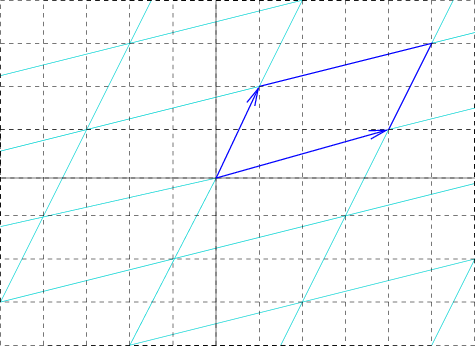
\includegraphics[width=0.40\textwidth]{Fundamental_parallelogram}
  \caption{\label{fig:FundParall}
A fundamental parallelogram spanned by (4,1) and (1,2) contains
${\Det \lattice = 7}$
points. Note that the far vertices (4,1), (1,2)  and (5,3) are not
counted, as they belong to other tiles.}
\end{figure}

A fundamental parallelogram spanned by (4,1) and (1,2) contains
\[
\Det\begin{pmatrix}
             4 & 1 \\
             1 & 2
      \end{pmatrix} = 7
\]
points, see \reffig{fig:FundParall}.

There is no unique fundamental pair; an infinite number of fundamental
pairs correspond to the same lattice. Any pair of fundamental
parallelograms is related by a modular group matrix
\(\in{SL}n{2}{\integers}\).  This equivalence of lattices underlies
many of the properties of elliptic functions (especially the Weierstrass
elliptic function - I think not relevant to us) and modular forms.

The abelian group \(\mathbb{Z}^2\) maps the complex plane
into the fundamental parallelogram. That is, every point \(z \in
\complex\) can be written as \(z=p+m\omega_1+n\omega_2\)
for integers $m$, $n$, with  a point $p$ in the fundamental
parallelogram.

If one identifies opposite sides of the parallelogram as
being the same, the fundamental parallelogram has the topology of a
torus; the quotient manifold
\(\complex/\lattice\) is a torus.
We are
possibly interested in functions on $\complex/$(lattice), functions on
$\complex$ with a certain periodicity condition. These doubly periodic,
meromorphic functions are called \emph{elliptic}.

\end{description}

\subsection{Integer lattice in $d$ dimensions}

Since we are interested in combinatorial rather than metric properties,
it suffices to consider the case of the standard integer lattice
$\integers^d\subset\reals^d$. The case of a general lattice \lattice\ in
$\reals^d$ reduces to that of $\integers^d$ by a change of the
coordinates.

\begin{description}

\item[2020-01-23 Predrag].

\HREF{https://en.wikipedia.org/wiki/Lattice_(group)} {wiki}:
{\em Lattice (group)}:
A lattice \lattice\ in \(\reals^d\)
has the form
\[
\lattice = \left\{\left. \sum_{i=1}^d a_i v_i \; \right\vert \; a_i \in\mathbb{Z} \right\}
\]
where
\beq
\{v_1,v_2,\cdots,v_d\}
\ee{integBas}
is a basis (or `integral basis') that defines the Bravais cell.
One convention is that an integral basis is ordered according to the
length of its elements; i.e. $|v_1|\leq|v_2|\leq\cdots\leq|v_d|$.

\HREF{https://en.wikipedia.org/wiki/Lattice_graph} {wiki}:
{\em A lattice graph},
mesh graph, or grid graph, is a graph whose drawing, embedded in
 $\reals^d$, forms a regular tiling.
In $d=2$ a lattice graph (or a square grid graph)
is the graph whose vertices correspond to the points in the plane with
integer coordinates.

The determinant (`discriminant' or `volume') of lattice $\lattice$ is
\beq
d(\lattice) = |\det(v_1|v_2|\cdots|v_d)|
\,.
\ee{lattVol}
The determinant is the reciprocal of the average density of points in the
lattice.
Different bases can generate the same lattice,
but the absolute value of the determinant
is uniquely determined by $\lattice$.
If one thinks of a lattice as dividing the whole of
\(\reals^d\) into equal polyhedra (copies of
an $d$-dimensional parallelepiped, the 'fundamental
region' of the lattice), then d($\lattice$) is equal to the $d$-dimensional
volume of this polyhedron.  This is why d($\lattice$) is sometimes called the
\emph{covolume} of the lattice.  If it equals 1, the lattice is called
unimodular.

The master of counting integer lattice points in various domains (and all
dimensions) is Alexander \HREF{http://www.math.lsa.umich.edu/~barvinok/}
{Barvinok}.
Barvinok \HREF{http://www.math.lsa.umich.edu/~barvinok/lectures.pdf}
{lectures} are very clear and simple. On p.~20 he defines the fundamental
parallelepiped, and then shows that

\textbf{Theorem 2}. The number of integer points in the fundamental
parallelepiped is equal to the volume of the parallelepiped.

Note that the fundamental parallelepiped is half-open, as indicated by
dashed lines in \reffig{Barvinok02fig81} so that the its translates form
a partition of the whole space.

Barvinok\rf{Barvinok02}
{\em A Course in Convexity}, \CBlibrary{Barvinok0}

Barvinok\rf{Barvinok08}
{\em Integer Points in Polyhedra}, \CBlibrary{Barvinok08} seems to
be a harder read, and not helpful for our integer lattice points counting.

1831 pages \HREF{http://www.csun.edu/~ctoth/Handbook/HDCG3.html}
{Handbook of Discrete and Computational Geometry} might be of some use.

\begin{figure}
  \centering
  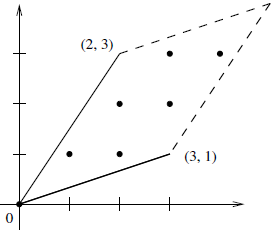
\includegraphics[width=0.35\textwidth]{Barvinok02fig81}
  \caption[]{\label{Barvinok02fig81}
A parallelepiped spanned by (3,1) and (2,3) contains
$\Det\begin{pmatrix}
             3 & 2 \\
             1 & 3
      \end{pmatrix} = 7$
points. Note that (3,1), (2,3) and the far vertex (5,4) are not counted.
Barvinok\rf{Barvinok02}~ Fig.~81.
  }
\end{figure}


Hademard's inequality.
Let $v_1,v_2,\cdots,v_d$ be any basis for $\lattice$. Then
\beq
d(\lattice)\leq |v_1| |v_2|\cdots|v_d|
\,,
\ee{reducedBas}
as the volume of a parallelepiped is
never greater than the product of the lengths of its sides. Hadamard's
inequality is an equality if and only if the basis vectors are orthogonal.
A theorem of Hermite says that every lattice has a basis that is
reasonably orthogonal (see \refeq{Holmin12-Hermite}), where the amount of
nonorthogonality is bounded solely in terms of the dimension. A
\emph{reduced basis} is an integral basis that minimizes the product of
lengths \refeq{reducedBas} over all bases of the lattice. Lattice
$\lattice$ is \emph{bounded} by T, if it has a reduced basis consisting of
vectors of length at most T.

\HREF{https://www.math.ucdavis.edu/~latte/software/packages/latte_current/manual_v1.7.2.pdf}
{LattE} is an ``Lattice point Enumeration'' program that  count  lattice
points  contained  in convex polyhedra defined by linear equations and
inequalities with integer coefficients\rf{DeLHTY04}. In 1994
Barvinok\rf{Barvinok94} gave an algorithm that counts lattice points in
convex rational polyhedra in polynomial time when the dimension of the
polytope is fixed. LattE counts the lattice points using multivariate
generating functions $P(a)$, $z^a=z^{a_1}z^{a_2}\cdots{z^{a_d}}$,
implementing Barvinok algorithm. At the end, $f(P)$ is written as a sum
of ``short'' rational functions.

Latte \HREF{https://www.math.ucdavis.edu/~latte/} {home page}.

\HREF{https://www.math.ucdavis.edu/~totalresidue/} {Maple} code.

Simplicial cone: Let \refeq{integBas} be a set of $k$ linearly
independent integral vectors in $\reals^d$, where $k\leq{d}$. Consider
simplicial cone $K$ and parallelepiped $S$ generated by \refeq{integBas},
\beq
K=\{\lambda_1 v_1+\lambda_2 v_2+\cdots+\lambda_k v_k\}
\,,\qquad 0\leq\lambda_i
\ee{coneK}
\beq
S=\{\lambda_1 v_1+\lambda_2 v_2+\cdots+\lambda_k v_k\}
\,,\qquad 0\leq\lambda_i<1
\ee{coneK1}
The generating function for the lattice points in $K$
equals\rf{Stanley09I}
    \PC{2020-01-25} {
I cannot find this formula in Stanley \rf{Stanley09I}, \CBlibrary{Stanley09I}.
    }
\beq
\sum_{\beta\in{K}\cap\integers^d}z^\beta=
\left(\sum_{\tau\in{S}\cap\integers^d}z^\tau\right)\prod_{i=1}^k \frac{1}{1-z^{v_i}}
\ee{coneKgenF}
A unimodular cone is a simplicial cone with all $\lambda=1$ which forms
an integral basis for the lattice
$\reals\{v_1,v_2,\cdots,v_k\}\cap\integers^d$. In this case the numerator
of the formula has a single monomial; in other words, the parallelepiped
has only one lattice point. The number of points in the parallelepiped
is obtained by
setting $z_i=1$ in the generating function
\beq
f(S;z)= \left(\sum_{\tau\in{S}\cap\integers^d}z^\tau\right)
\ee{noPinS}
However, the generating function is not constructed by enumerating all
the integer points in $S$, but rather as a signed sum of rational
functions that can be derived from the description of $S$. They all count
points in a general polyhedron; counting them in a parallelepiped should
be a simple special case, but I have not seen that discussed separately.

Note that this count does not identify opposing sides of the
parallelepiped.

If we need to enumerate periodic points one-by-one, John Voight
\HREF{https://mathoverflow.net/questions/57773/listing-lattice-points-in-a-simplex}
{mathoverflow} question might be a start.

\HREF{http://www.stumblingrobot.com/2015/07/15/prove-a-formula-for-the-area-of-a-polygon-whose-vertices-are-lattice-points/}
{Stumbling Robot} derives the area of a polygon whose vertices are
lattice points.

The study of integer points in convex polyhedra is motivated by questions
such as "how many nonnegative integer-valued solutions does a system of
linear equations with nonnegative coefficients have" or "how many
solutions does an integer linear program have".

\HREF{https://en.wikipedia.org/wiki/Minkowski\%27s_theorem} {wiki}:
{\em Minkowski's theorem} relates the number $d(\lattice)$ and the volume of
a symmetric convex set $S$ to the number of lattice points
contained in $S$. The number of lattice points contained in a
polytope all of whose vertices are elements of the lattice is
described by the polytope's Ehrhart polynomial. Formulas for some of
the coefficients of this polynomial involve $d(\lattice)$ as well.

\HREF{https://en.wikipedia.org/wiki/Ehrhart_polynomial} {wiki}:
An integral polytope has an associated {\em Ehrhart polynomial} that
encodes the relationship between the volume of a polytope and the number
of integer points the polytope contains. A generating function for the
Ehrhart polynomials, or the Ehrhart series is a rational function - this
suggest that we should able to convert this series into a zeta function.
This wiki has some intriguing explicit examples.

\item[2020-09-18 Predrag]
Subramaniam and Balani have an
\HREF{http://home.iitk.ac.in/~anandh/E-book/} {E-book}
with a cute chapter on
\HREF{http://home.iitk.ac.in/~anandh/E-book/lattice.ppt} {lattices},
but it standard Bravais lattice crystallography, of no use to us. Ignore

\item[2020-07-31 Predrag]
The \catlatt\ \jacobianOrb\ \refeq{catalattLxT}
in the {\HillDet} $\det{\jMorb}$ computation for a
$\BravCell{\speriod{}}{\period{}}{0}$ rectangular Bravais cell is
expressed naturally and spacetime symmetrically in terms of `horizontal',
`vertical' translation generators $\shift_{1}$, $\shift_{2}$.

I expect that for an arbitrary Bravais cell, such as
\reffig{Barvinok02fig81}, the corresponding translation generators should
act along the `integral basis' vectors \refeq{integBas} that define the
Bravais cell $\lattice$, \ie, the \catlatt\ {\HillDet} should be given by
\beq
\det{\mathbf{\jMorb}}=\det({\mathbf{\jMorb}\lattice)}/\det{\lattice}
\,,
\ee{HillDetAnyCell}
where \catlatt\ \jacobianOrb\ ${\mathbf{\jMorb}}$ should be expressed in
terms of translations along the Bravais cell basis vectors, and the
{\HillDet} should be expressed terms of invariant quantities that can be
constructed from them. The simplest is the volume \refeq{lattVol}, the
others are presumably related to traces $\tr\lattice^k$ and the
corresponding subvolumes. Not sure what they are, but someone has surely
thought about that. My understanding is summarized in
\HREF{http://birdtracks.eu/version9.0/GroupTheory.pdf\#section.6.4}
{birdtracks.eu}.

Han and I have an answer of asymmetric form for the \jacobianOrb\
\refeq{catalattLxT} for a tilted Bravais domain (\rpo)
\refeq{catalattLxTrop}, with the relative periodicity all in the
`comoving frame' translation generator
$\shift_{1}^{-\tilt{}/\period{}}\otimes\shift_2$.

This space-time asymmetry is a consequence of choosing the Hermite normal
form \refeq{Holmin12-Hermite} to define the Bravais cell. So - even
though we are computing the representation-independent determinants, we
do not have an invariant statement of cell's `tilt'. There must be a more
elegant answer to this.
Some of this discussion is in the {\bf 2020-07-11 Predrag} post,
around eq.~\refeq{DudMer84(2.106)}.

But that might lead us too deep into the role that prime numbers play in
characterizing equivalent Bravais cells $\lattice$ and their volumes.
Whenever you result depends on factorization in primes, it is time to
sound a potentially deep number theory {\color{red}red alert :)}

\item[2020-01-23 Predrag]
\HREF{https://cims.nyu.edu/~regev/} {Oded Regev} is good on this - will
post more links. He uses
Micciancio and Goldwasser\rf{MicG0l02}
{\em Complexity of Lattice Problems - A Cryptographic Perspective}
\CBlibrary{MicG0l02} as
his course textbook.

\HREF{https://cims.nyu.edu/~regev/teaching/lattices_fall_2004/ln/introduction.pdf}
{Oded Regev}: Definition~5 defines $d(\lattice)$, the determinant of a
lattice in terms of the Bravais basis that might be useful to us.

\HREF{https://cs.nyu.edu/courses/spring13/CSCI-GA.3033-013/}
{Lattices, Convexity and Algorithms} lecture notes from
\HREF{https://cs.nyu.edu/courses/spring13/CSCI-GA.3033-013/lectures/lecture-1.pdf}
{2013} might be better. Check out
``Gram Schmidt Orthogonalization,'' which I think is his construction
of the Hermite normal basis, and
``Equivalence of Lattice Definitions.''
Also check out his {\em Fundamental Parallelepiped and the Determinant}
\HREF{https://cs.nyu.edu/courses/spring13/CSCI-GA.3033-013/lectures/lecture-3.pdf}
{lecture}.

\item[2020-12-12 Predrag]                                          \toCB
Haviv and Regev \arXiv{1311.0366} address the Lattice Isomorphism
Problem (LIP). I like their definitions.

Two lattices $\lattice_1$ and $\lattice_2$ are
isomorphic if there exists an orthogonal linear transformation
mapping $\lattice_1$ to $\lattice_2$.

An {\em orthogonal} linear transformation (or {\em isometry}) $O : V_1
\rightarrow V_2$ is a linear transformation that preserves inner
products, that is, $\langle x, y\rangle = \langle O(x), O(y)\rangle$ for
every $x,y \in V_1$. For a set $A \subseteq V_1$ we use the notation
$O(A) = \{ O(x) \mid x \in A\}$.

For a matrix $B$ we denote its $i$th column by $b_i$, and $O(B)$ stands
for the matrix whose $i$th column is $O(b_i)$.
${\mathop{\mathrm{span}}}(B)$ stands for the subspace spanned
by the columns of $B$.

%\label{fact:Gram}
Let $B$ and $D$ be two matrices satisfying $B^T \cdot B = D^T \cdot D$.
Then there exists an orthogonal linear transformation
$O:{\mathop{\mathrm{span}}}(B) \rightarrow {\mathop{\mathrm{span}}}(D)$
for which $D = O(B)$.

An $m$-dimensional {\em lattice} $\lattice \subseteq \R^m$ is the set of
all integer combinations of a set of linearly independent vectors
$\{b_1,\ldots,b_n\} \subseteq \R^m $, i.e.,
$\lattice=\{\sum_{i=1}^{n}{a_i b_i}~|~\forall i.~a_i \in \integers\}$. The set
$\{b_1,\ldots,b_n\}$ is called a {\em basis} of $\lattice$ and $n$, the
number of vectors in it, is the {\em rank} of $\lattice$. Let $B$ be the
$m$ by $n$ matrix whose $i$th column is $b_i$. We identify the matrix and
the basis that it represents and denote by $\lattice(B)$ the lattice that
$B$ generates.
% The norm of a basis $B$ is defined by $\|B\| = \max_{i}{\|b_i\|}$.



A basis of a lattice is not unique: two bases $B_1$
and $B_2$ generate the same lattice of rank $n$ if and only if $B_1 = B_2
\cdot U$ for a {\em unimodular} matrix $U \in \integers^{n \times n}$,
i.e., an integer matrix satisfying $|\det(U)|=1$.

The determinant of a lattice $\lattice$ is defined by
\beq
\det(\lattice)=\sqrt{\det(B^T B)}
\,,
\ee{detLat}
where $B$ is a basis that generates $\lattice$.
$\det(\lattice)$ is independent of the choice of the basis. A
set of (not necessarily linearly independent) vectors that generate a
lattice is called a {\em generating set} of the lattice.

A lattice ${\cal M}$ is a {\em sublattice} of a lattice $\lattice$ if
${\cal M} \subseteq \lattice$, and it is a {\em strict sublattice} if
${\cal M} \subsetneq \lattice$. If a lattice $\lattice$ and its
sublattice ${\cal M}$ span the same subspace, then the {\em index} of
${\cal M}$ in $\lattice$ is defined by $|\lattice : {\cal M}| =
\det({\cal M})/\det(\lattice)$. If ${\cal M}$ is a sublattice of
$\lattice$ such that $|\lattice : {\cal M}|=1$ then ${\cal M}=\lattice$.

They define lattices by their \emph{Gram matrices}.
The {\em Gram matrix} of a matrix $B$ is defined to be the matrix
\beq
G = B^T \cdot B
\,,
\ee{Gram1}
or equivalently,
\beq
G_{ij} = \langle b_i , b_j \rangle
\,,\qquad \mbox{for every } i \mbox{ and } j
\,.
\ee{Gram2}
A Gram matrix specifies a basis only up to rotation.
\index{Gram matrix}

In the Lattice Isomorphism Problem the input consists of two Gram
matrices $G_1$ and $G_2$, and the goal is to decide if there exists a
unimodular matrix $U$ for which $G_1 = U^T \cdot G_2 \cdot U$.

The {\em dual lattice} of a lattice $\lattice$, denoted by $\lattice^*$,
is defined as the set of all vectors in
${\mathop{\mathrm{span}}}(\lattice)$ that have integer inner product with
all the lattice vectors of $\lattice$, that is,
\[
\lattice^* = \{u \in
{\mathop{\mathrm{span}}}(\lattice)~|~\forall v \in \lattice.~\langle u,v
\rangle \in \integers \}
\,.
\]
The {\em dual basis} of a lattice basis $B$ is
denoted by $B^*$ and is defined as the one which satisfies $B^T \cdot B^*
= I$ and ${\mathop{\mathrm{span}}}(B)={\mathop{\mathrm{span}}}(B^*)$,
that is, $B^* = B(B^T B)^{-1}$. It is well known that the dual basis
generates the dual lattice, i.e., $\lattice(B)^* = \lattice(B^*)$.

The relations between parameters of lattices and parameters of their dual
are known as {\em transference theorems}.

\item[2020-02-14 Predrag]
Given a nondegenerate lattice $\lattice$, we can construct an invariant by
choosing a basis, and taking the determinant of the matrix whose (i,j)
entry is the inner product of the i-th basis vector with the j-th basis
vector. The matrix is called the Gram matrix of the basis, and the
determinant is a rough measure of how loosely packed the lattice vectors
are in $\lattice\otimes\mathbb{R}$.

\item[2020-02-14 Predrag]
I have run (once) into `fundamental parallelepiped' being called
`fundamental parallelotope'.

\item[2020-12-12 Predrag]
For our choice of Hermite normal form \refeq{Holmin12-Hermite2d},
\refeq{HermiteBasis}, the {Gram matrix} \refeq{Gram1} is
\beq
G =
\left[\begin{array}{cc}
\speriod{}^2      & \speriod{}\tilt{} \\
\speriod{}\tilt{} & \speriod{}^2  + \period{}^2
\end{array}\right]
\,.
\ee{Gramin2d}

\item[2020-09-08 Predrag]
%\HREF{https://cseweb.ucsd.edu/classes/wi12/cse206A-a/lec1.pdf} 2012 course
\HREF{http://cseweb.ucsd.edu/classes/sp14/cse206A-a/lec1.pdf} % 2014 course
{Daniele Micciancio} is very economical. I propose we follow his exposition, and
use Micciancio and Goldwasser\rf{MicG0l02} {\em Complexity of Lattice
Problems - A Cryptographic Perspective} \CBlibrary{MicG0l02}. They
say (I have not looked at any of these, so they might be even better
than Micciancio and Goldwasser, for our purposes):

``Classical references about lattices are Cassels\rf{Cassels59} (or 1971)
\CBlibrary{Cassels59} and Gruber and Lekerkerker\rf{GruLek87}
\HREF{http://ChaosBook.org/library/GruLek871.djv} {(click here)}. Another
very good reference is Siegel\rf{Siegel89} \CBlibrary{Siegel89}. For a
brief introduction to the applications of lattices in various areas of
mathematics and science the reader is referred to (Lagarias 1995) and
(Gritzmann and Wills 1993), which also touch some complexity and
algorithmic issues. A very good survey of algorithmic application of
lattices is (Kannan 1987a).''

Lattices are regular arrangements of points in Euclidean space.  The
simplest example of lattice inn-dimensional space is $\integers^d$, the
set of all $d$\dmn\ vectors with integer entries. More generally, a
lattice is the result of applying a nonsingular linear transformation
$B\in{\reals^{m\times{d}}}$ to the integer lattice $\integers^d$, to
obtain the set
\(
B(\integers^m) =\{Bx:x\in \integers^d\}
\,.
\)
etc. - you fill it in.

To Han: can you replace our `Bravais' by Micciancio and
Goldwasser\rf{MicG0l02} lattice definitions?

Is the `Hermite
normal form'the same as the `Gram-Schmidt orthogonalization method'?

\item[2020-09-11 Han]
See \refsect{s:BravaisLatt}.
Gram Schmidt Orthogonalization constructs orthogonal with
basis vectors whose tips are not on $\integers^d$ lattice; not Hermite
normal form, forget it.


    	\HLpost{2018-01-31}{
The similarity transformation ${\bf S}$ that maps \refeq{ArnoldCat}
into \refeq{PerViv:2confRepMat},
\beq
{\bf A}
=\MatrixII{2}{1}
          {1}{1}
\,,\qquad
{\bf B}
=\MatrixII{0}{1}
          {-1}{3}
\,,
\ee{HLsimilarityB}
is
\beq
{\bf B} = {\bf S}^{-1}{\bf A}{\bf S}
\,,
\ee{HLsimilarityC}
where
\[
{\bf S} = {\bf S}^{-1}
        =\MatrixII{-1}{2}
				   {0}{1}
\,.
\]
}

\PCpost{2018-04-27}{
    % mathematica Matrix[{-1,2},{0,1}] Matrix[{1,1},{1,0}] Matrix[{-1,2},{0,1}]
Note that $\det {\bf S} = -1$. Why? That can be fixed by multiplying it
by $\ii$, but why? It is also not unique, one could,  for example, use
\[
{\bf S'} = {\bf S'}{}^{-1}
        =
\MatrixII{0}{-1}
		  {1}{0}
\MatrixII{-1}{2}
		  {0}{1}
\MatrixII{0}{1}
		{-1}{0}
        =
\MatrixII{1}{ 0}
		{-2}{-1}
\,.
\]
For a systematic discussion, see sect.~4. {\em Global versus local conjugacy
and orbit statistics} of Baake \etal\rf{BaRoWe08}, and sect.~2.5.  {\em
Results for d = 2} of Baake \etal\rf{BaNeRo13} {\em Orbit structure and
(reversing) symmetries of toral endomorphisms on rational lattices}. The main
point (for us) is that maps that are in the same conjugacy class need to have
3 invariants in common; the trace, the determinant, and the mgcd (the matrix
greatest common denominator). For the Thom-Arnol'd cat map \refeq{ArnoldCat},
$mgcd(A) = 1$

Baake \etal\rf{BaNeRo13} discus ``pretails''
to \po s at length.
}

\PCpost{2018-04-27}{
Next, one can transform Arnold cat map ``square root'' ${\bf C}$ (or,
according to Baake \etal\rf{BaRoWe08}, the `classic'' or golden orientation
reversing cat map, or the Fibonacci cat map\rf{BaNeRo13}, with $\det(\bf
C)=-1$)
\beq
{\bf A}={\bf C}^2\,,\qquad
{\bf C} = \MatrixII
 {1} {1}
 {1} {0}
\ee{AABHM99-44HL}
to the \PV\ version
\beq
{\bf B} = {\bf \tilde{C}}^2
\,,\quad
{\bf \tilde{C}} = {\bf S}^{-1}{\bf C}{\bf S}
 = \MatrixII
 {-2} {1}
 {-1} {1}
\,.
\ee{HLsimilarityS}
As noted in \refeq{AABHM99-46}, taking this ``square root'' expresses the
zeta function as a product of a time-reversal pair of zeta's. ${\bf B}$ and
${\bf\tilde{C}}$ have the same eigenvectors, but as $\det {\bf\tilde{C}}=-1$,
one of the stability multipliers is a negative square root of the ${\bf B}$
multipliers \refeq{catEigs},
\beq
\tilde{\ExpaEig} = \tilde{\ExpaEig}_1 = \frac{1 + \sqrt{5}}{2} % = 2.6180
\,,\qquad
\tilde{\ExpaEig}_2 = \frac{1 - \sqrt{5}}{2} % = 2.6180
\,.
\ee{goldenMltpl}
The issue of reversibility seems complicated\rf{BaNeRo13}.
When $M\in\mbox{SL}(2,\integers)$, also its inverse is in
$M^{-1}\in\mbox{SL}(2,\integers)$, and $M$ and $M^{-1}$ share the same determinant,
trace and mgcd:
\[
{\bf M} = \MatrixII
 {a} {b}
 {c} {d}
\,,\qquad
{\bf M}^{-1} = \MatrixII
 {~d} {-b}
 {-c} {~a}
\,.
\]
The the golden (Fibonacci\rf{BaNeRo13}) cat map \refeq{AABHM99-44HL} is not
reversible in $\mbox{GL}(2,\integers)$ (while its square $A$
is\rf{BaNeRo13}).
}



\PCpost{2020-02-19}{
\emph{Linear recurrences with constant coefficients: the multivariate case}
by
Mireille Bousquet-M{\'e}lou1a and Marko Petkov{\v{s}}ek,
\HREF{https://doi.org/10.1016/S0012-365X(00)00147-3} {(DOI)}
has the right feel and a few 2\dmn\ integer lattice recurrences and
the corresponding functional equations,
but I do not see how to apply it to the 2\dmn\ \catlatt.
    }

\item[2020-07-11 Predrag]
Woods\rf{Woods12} (2012) \CBlibrary{Woods12} is very clear, what follows
is excerpted from it. As Woods says, his starting chapters are taken
from Lim\rf{Lim90} {\em Two-dimensional Signal and Image Processing}
\CBlibrary{Lim90} \CBlibrary{BecRob07}, who copies from Dudgeon and
Mersereau\rf{DudMer84} (1984) {\em Multidimensional Digital Signal
Processing} \CBlibrary{DudMer84} which cover the same ground.
\\

A 2{\dmn} field $\field_{n \zeit}$ is periodic with period
$\BravCell{\speriod{}}{\period{}}{0}$, if the
following equalities hold for all integers $n$, $\zeit$:
\beq
\field_{n\zeit} = \field_{n + \speriod{}, \zeit}
                 = \field_{n, \zeit+ \period{}}
\,,
\ee{Woods12p6}
where \speriod{} and \period{} are positive integers.
This type of periodicity occurs often for 2{\dmn} signals and is referred to
as \emph{rectangular periodicity}. We call the resulting period the
\emph{rectangular period}.

Given a periodic function, the period effectively defines a basic cell in
the plane, which can be repeated to form the function over all integers
$n$, $\zeit$. As such, we often want the minimum size unit cell for
efficiency of both specification and storage. In the case of the
rectangular period, we seek the smallest nonzero integers that will
suffice for $\BravCell{\speriod{}}{\period{}}{0}$ to form this basic
cell.

\textbf{Horizontal Wave.}
Consider the sine wave
\(
\field_{n\zeit}  = \sin(2\pi n/4)
\,.
\)
The horizontal period is $\speriod{}=4$. In the vertical direction, the
signal is constant, so we can use any positive integer $\period{}$.
The smallest such value is $\period{}=1$. Thus the rectangular period is
$\BravCell{\speriod{}}{\period{}}{0}=\BravCell{4}{1}{0}$,
and the basic cell consists of the set of points
\(
\{({n\zeit}) = [(0,0),(1,0),(2,0),(3,0)]\}
\)
 or any translate of this set.

In general,  `periodicity' refers to a repetition of blocks, not
necessarily rectangular blocks or blocks occurring on a rectangular
repeat grid, with the periodicity represented with two integer vectors,
\[
v_1=\begin{pmatrix}
  \speriod{}\\
  c_{21}{}
  \end{pmatrix}
  \,,\qquad
v_2=\begin{pmatrix}
  \tilt{}\\
  \period{}
  \end{pmatrix}
  \,.
\]
While they note the nonuniqueness of Bravais cells with respect to
unimodular transformations, image processing textbooks seem not to use
the Hermite normal form \refeq{Holmin12-Hermite} to eliminate $c_{21}$.

The 2{\dmn} field $\field_{n \zeit}$ is periodic with period
\(
(v_1,v_2) = \Lambda
\)
if the following hold for all integers  $n$, $\zeit$:
\beq
\field_{n\zeit} = \field_{n + \speriod{}, \zeit+c_{21}}
                 = \field_{n + \tilt{}, \zeit+ \period{}}
\,,
\ee{Woods12p8}
To avoid degenerate cases, restrict the integers in $v_j$ with the
condition
\[
\det(v_1,v_2)\neq0
\,.
\]
``We leave it to the reader to show that'' the number of samples in this
region is $\det\Lambda$, \ie, the absolute value of the determinant of
the periodicity matrix gives the number of samples of $\field_{{\bf n}}$
contained in one period.

The matrix $\Lambda$ is called the \emph{periodicity matrix}. In matrix
notation, the periodic field satisfies
\[
\field_{{\bf n}} = \field_{{\bf n}+\Lambda{\bf r}}
\,,\qquad {\bf r}= \begin{pmatrix} r_{1}\\r_{2}\end{pmatrix}
\,.
\]
Two integer vectors ${\bf m}$ and ${\bf n}$ are \emph{congruent} with
respect to the matrix modulus $\Lambda$ if
\(
{\bf m}= {\bf n} + \Lambda{\bf r}
\)
for some integer vector ${\bf r}$.

In the case that $\Lambda$ is a diagonal
matrix, $\field_{{\bf n}}$ is \emph{rectangularly periodic}.

If $P$ is any integer matrix, then $P\Lambda$ is also be a periodicity
matrix for $\field_{{\bf n}}$. Thus the periodicity matrix is not unique
for any periodic sequence.

A matrix $E$ for which $\det E = 1$ is called a \emph{unimodular matrix}.
$E^{-1}$ is then also a unimodular matrix. Unimodular matrices are the
only integer matrices whose inverses are also integer matrices. If
$\det\Lambda$ is a prime number, we will say that $\Lambda$ is a
\emph{prime matrix}. If $\Lambda$ is neither prime nor unimodular, we say
that it is \emph{composite}, and can be decomposed, nonuniquely - up to
a unimodular transformation - into a
product of two non-unimodular matrices
    \index{unimodular matrix}
\beq
\Lambda=PQ
\,.
\ee{DudMer84(2.106)}
If either $P$ or $Q$ is composite, one continues the process, until
$\det\Lambda$ is the product of its prime factors.

Dudgeon and Mersereau\rf{DudMer84} then explain clearly how to get the
``quotient'' $Q$ when ``dividing'' by $P$. $|\det\Lambda|/|\det Q| =
|\det P|$ is then the number of cosets. In the image-processing, Fourier
transforms trade this non-prime factorization is known as
``decimation-in-time Cooley-Tukey FFT algorithm,'' ``twiddle factors,''
and ``butterflies.''
     \PC{2020-07-15} {
     Use this to define prime factorization in \refref{CL18}?
     }

{\bf Example} \Reqv\ field
\(
\sin [2\pi (n/8+\zeit/16)]
\)
is constant along the line
\(
2n+\zeit=16
\,.
\)
The basis vectors are
\[
v_1=\begin{pmatrix}
  4\\8
    \end{pmatrix}
  \,,\qquad
v_2=\begin{pmatrix}
  ~1\\-2
     \end{pmatrix}
  \,,\qquad
\mbox{with } \det\Lambda=16
  \,.
\]

\textbf{Definition 1.1-1: Linear System} $[\cdots]$ \\

\textbf{Definition 1.1-2: Shift Invariance} $[\cdots]$

``Linear shift-invariant discrete systems are generally implemented using
difference equations. Although multidimensional difference equations
represent a generalization of 1\dmn\ difference equations, they are
considerably more complex and are, in fact, quite different. A number of
important issues associated with multidimensional difference equations,
such as the direction of recursion and the ordering relation, are really
not issues in the 1\dmn\ case.

$[\cdots]$ they define multidimensional recursive systems and consider
the issues associated with multidimensional difference equations;
$[\cdots]$  define the multidimensional Z-transform.
''
\\

\textbf{2{\dmn} Convolution}
If a system is \emph{linear shift-invariant} (LSI), then  $[\cdots]$
%
the field $h$ is called the LSI system's \emph{impulse response}.
 $[\cdots]$
He defines the 2{\dmn} convolution operator  $[\cdots]$

\textbf{Properties of 2{\dmn} Convolution or Convolution Algebra}  $[\cdots]$
All 5 properties of convolution hold for any 2{\dmn} fields $x, y$, and $z$,
for which convolution is defined (i.e., for which the infinite sums
exist). His Figure 1.1-9 illustrates a convolution.
\\

\textbf{Stability in 2{\dmn} Systems}
    \PC{2020-07-11}{I do not understand BIBO, but maybe we should?}
Stable systems are those for which a small change in the input gives a
small change in the output. We define bounded-input bounded-output (BIBO)
stability for 2{\dmn} systems analogously to that in 1{\dmn} system
theory. A spatial or 2{\dmn} system will be stable if the response to
every uniformly bounded input is itself uniformly bounded. For an LSI
system the condition is equivalent to the impulse response being
absolutely summable,
\beq
\sum_{k1,k2} |h_{k1,k2}| <\infty
\,.
\ee{Woods12(1.1-3)}

Sect.~1.2 \textbf{2{\dmn} discrete-space Fourier transform} The Fourier
transform is important in 1{\dmn} signal processing because it
effectively explains the operation of linear time-invariant (LTI) systems
via the concept of frequency response, \ie, the Fourier transform of the
system impulse response. While convolution provides a complicated
description of the LTI system operation, with the input at all locations
$n$ affects the output at all locations, the frequency response provides
a simple interpretation as a scalar weighting in the Fourier domain,
where the output at each frequency $\omega$ depends only on the input at
that same frequency. A similar result holds for 2{\dmn} systems that are
LSI.

{\bf 2020-07-15 Predrag} Note that the discrete Fourier transform of a
Bravais lattice always carries the prefactor $1/\det\Lambda$. Going back
involves a volume $(2\pi)^d$.

\textbf{Definition 1.2-1: 2{\dmn} Fourier Transform} $[\cdots]$
In the 2{\dmn} Fourier transform the frequency variable $\omega_1$ is
called \emph{horizontal frequency}, and the variable $\omega_2$ is called
\emph{vertical frequency}.
 $[\cdots]$
As $n$, $\zeit$ are integers, the 2{\dmn} Fourier transform is periodic
with rectangular period $2\pi\times2\pi$, and only needs be calculated
for one period, usually taken to be $[-\pi,\pi]\times[-\pi,\pi]$.

$[\cdots]$
the 2{\dmn} Fourier transform is a \emph{separable operator}, because it
can be performed as the concatenation of 1{\dmn} operations on the rows
followed by 2{\dmn} operations on the columns.

\textbf{Inverse 2{\dmn} Fourier Transform} $[\cdots]$ \\

\textbf{Fourier Transform of 2{\dmn} or Spatial Convolution}\\
\textbf{Theorem 1.211: Fourier Convolution Theorem} $[\cdots]$ \\

$[\cdots]$
As a 2{\dmn} or spatial LSI system is characterized by its impulse
response $h_{n,\zeit}$, its frequency response $H_{\omega_1,\omega_2}$ suffices to
characterize such a system. And the Fourier transform Y of the output equals the product
of the frequency response H and the Fourier transform X of the input. When the
frequency response H takes on only values 1 and 0, the system is an \emph{ideal filter},
filtering out some frequencies and passing others unmodified.
More generally, the term filter include all such LSI systems, and
has been extended to shift-variant and even nonlinear systems through the concept of
the Voltera series of operators.
    \PC{2020-07-11}{
`Voltera series of operators'? Defined in
S. Thurnhofer and S. K. Mitra, {\em A General Framework for Quadratic
Volterra Filters for Edge Enhancement}, IEEE Trans. Image Process., vol.
5, June, pp. 950-963, 1996.
    }

\textbf{Some Important Properties of the FT Operator} $[\cdots]$ \\

\textbf{Some Useful Fourier Transform Pairs} $[\cdots]$ \\

\textbf{Example 1.2-4: Fourier Transform of Separable Signal} $[\cdots]$ \\

\textbf{Symmetry Properties of the Fourier Transform} $[\cdots]$ \\

Generally, we think of the Fourier transform as the evaluation of the
Z-transform on the unit polycircle $\{|z_1| = |z_2| = 1\}$; however, this
assumes the polycircle is in the region of convergence of $X(z_1,z_2)$,
which is not always true.

  $[\cdots]$
linear shift-invariant systems with sinusoidal excitations are naturally
described by the Fourier transform. The Z-transform is a generalization
of the Fourier transform which allows us to treat exponential inputs.

  $[\cdots]$
Exponentials of the form $\ssp_{n_1 n_2} = z^{n_1}z^{n_2}$ are
eigenfuctions of 2\dmn\ linear shift invariant systems.

 The 2\dmn\ Z-transform of a discrete field \Xx\ is defined as
\beq
\Xx_{z_1z_2}^Z =
\sum_{n_1=-\infty}^{\infty}\sum_{n_2=-\infty}^{\infty}
 \ssp_{n_1 n_2} z_1^{-n_1}z_2^{-n_2}
%    \continue
%    \ceq
\,.
\label{DudMer84(4.18)}
\eeq

\textbf{Example 3.4-5: Comparison of Fourier Transform and Z-Transform}
$[\cdots]$ \\

The Fourier transform is not strictly a subset of the Z-transform,
because it can use impulses and other singularity functions, which are
not permitted to Z-transforms.

  $[\cdots]$
The Fourier transform is used primarily to describe signals and to
describe the actions that systems will have on them. The Z-transform is
used to describe systems and to provide an additional tool for
manipulating difference equations. While the 2\dmn\ Z-transform is related
to its l\dmn\ counterpart, the two transforms are actually quite
different.

For $z_1 = e^{i\omega_1}$, $z_2 = e^{i\omega_2}$ the Z-transform reduces
to the Fourier transform. The corresponding surface in the Z-domain is
the called 2\dmn\ unit \emph{bicircle}. 2\dmn\ Z-transform
converges on the \emph{Reinhardt domain}, the 2\dmn\  analog of the annulus
for 1\dmn\ case.
\\



\renewcommand\speriod[1]{{\ensuremath{\ell_{#1}}}}  %continuous spatial period
\renewcommand\period[1]{{\ensuremath{\ell_{#1}}}}  %continuous time period

\item[2020-02-23 Predrag]
Continuing on the multivariate generating functions,
the {\em integer-point transform} introduced in this
 textbook in integer lattices counting:
Beck and Robins\rf{BecRob07}
{\em Computing the Continuous Discretely},
\CBlibrary{BecRob07}, might be helpful:

% clip & paste from \arxiv{1509.03121}
Let ${\bf a} =(a_1,\dots ,a_d)$ $\in\integers^d$ be an integer point. The
Laurent monomial ${\bf z}^{\bf a}$  is defined as
\beq
{\bf z}^{\bf a}
:=z_1^{a_1}z_2^{a_2}\cdots z_d^{a_d}, \quad {\bf z}^{\bf{0}}:=1
\ee{BecRob07:LaurMon}
 where
${\bf{0}}:=(0,0,\dots ,0)$. For a given rational cone or rational
polytope $S\subset \reals^d$,
\beq
\sigma_S({\bf z})
    =\sigma_S(z_1,z_2,\dots ,z_d)
   :=\sum_{{\bf a}\in S\cap \integers^d}{\bf z}^{\bf a}
\ee{BecRob07:IntPoTrnsf}
is called the {\em integer-point transform} of $S$.
The function $\sigma_S$ lists all integer points in $S$ not as a
list of vectors, but as a sum of monomials. This
$\sigma_S$ also goes by the name \emph{moment generating function} or
simply \emph{generating function} of $S$.
    \index{integer-point transform}
    \index{moment generating function}\index{generating function}

%%%%%%%%%%%%%%%%%%%%%%%%%%%%%%%%%%%
\begin{figure}
  \centering
  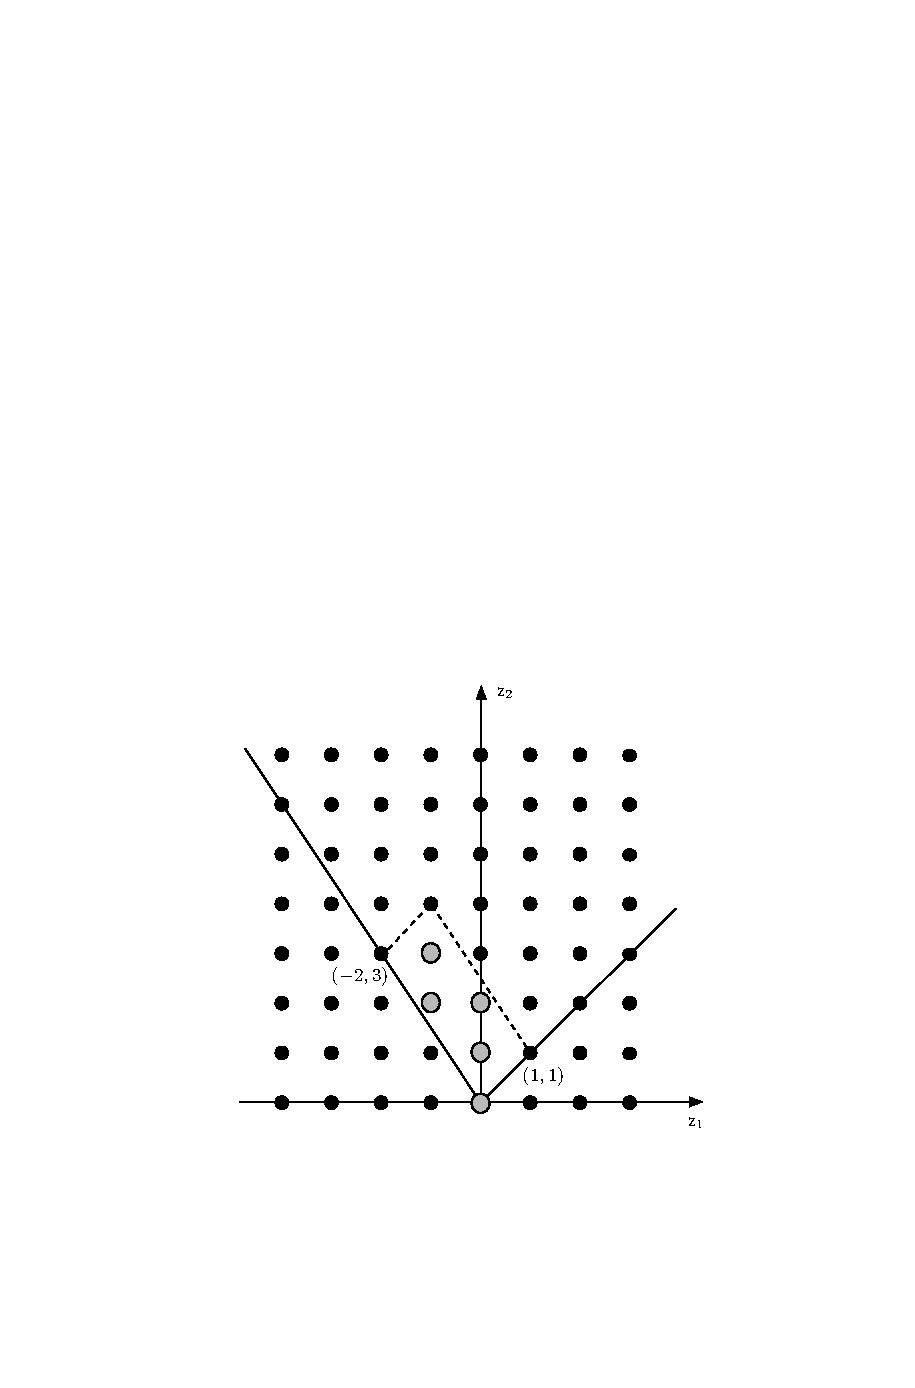
\includegraphics[width=0.40\textwidth]{BecRob07fig3-3}
  \caption{\label{BecRob07:fig3-3}
The cone ${\cal K}$ and its fundamental parallelogram,
fig~3.3 from \refref{BecRob07}.
    }
\end{figure}
%%%%%%%%%%%%%%%%%%%%%%%%%%%%%%%%%%%%

They start with the usual trivial example of a geometric series in
Example 3.3, and work out a 2\dmn\ $\{(1, 1),(-2, 3)\}$ Bravais lattice
in example Example 3.4, see \reffig{BecRob07:fig3-3}. They call the
$\reals^2$ interior of the half-open Bravais cell `fundamental
parallelogram $\Pi$', and tile the two-dimensional cone ${\cal K}$ with
its non-negative translations. That results in the rational polynomial
formula for the integer-point transform of the cone ${\cal K}$
\beq
\sigma_{\cal K}({\bf z}) =
\frac{1 + z_2 + z_2^2 + z_1^{-1}z_2^2 + z_1^{-1} z_2^3}
     {(1 - z_1z_2)(1 - z_1^{-2} z_2^3)}
\ee{BecRob07:examp3-4}
of the form that I had suggested to Han for
the \catlatt.
\medskip

Check also:
\begin{itemize}
  \item
{\bf 2020-03-02 Predrag} notes below, on Wilf\rf{Wilf94}
sect.~1.5 {\em Two independent variables}.
  \item
\emph{Characteristic function} or ``five-point stencil''
\refeq{FGHLW74:charFunct2d}
\end{itemize}


\item[2020-03-03 Predrag]
OK,
the {\fundPip} determinant \refeq{lattVol} counts integer points
\beq
N_\cl{} = |\Det\jMorb| = |\Det(v_1|v_2|\cdots|v_\cl{})|
\,.
\ee{lattVol1}
What does
\(
\Tr\jMorb
\)
do? That is also an invariant under $SLG(\cl{})$ lattice transformations.


\end{description}


\subsection{Primitive parallelogram}

\begin{description}

\item[2020-01-25 Predrag]

A lattice vector is called \emph{primitive},  if there is no other
lattice points on the segment between  0  and the tip.

or:

% from Holmin  	10.1007/s00605-013-0518-x,  	\arXiv{1211.2716}
An integer vector $v\in\integers^d$ is {\em primitive}
if it cannot be written as an integer multiple $m\neq 1$ of some other
integer vector $w\in\integers^d$.
\index{primitive vector}

or:

A lattice point is a primitive lattice point if it is not a multiple of any
other lattice point, that is, the greatest common divisor of its
coordinates is one.

or:

A primitive lattice point is a
lattice point visible from the origin.

Let $A$ be an integer $[d\times d]$-matrix with
nonzero determinant $k$ and primitive row vectors.
The common divisors of the entries of each row
of $A$ are preserved under multiplication on
the right by any matrix $X\in{SL}n{d}{\integers}$.

A lower triangular integer matrix
\beq
  C\defeq \begin{pmatrix}
  c_{11}&0&\cdots&0\\
  c_{21}&c_{22}&\ddots&0 \\
  \vdots&&\ddots&0\\
  c_{d1}&\cdots&c_{d(d-1)}&c_{dd}
  \end{pmatrix}
\ee{Holmin12-Hermite}
is said to be in (lower) {\em Hermite normal form} if $0<c_{11}$ and
$0\leq c_{ij}<c_{ii}$ for all $j<i$.

 I would prefer the vectors to
be column vectors, as in Lind \refeq{HLreciprocal7}.
In particular, in the case of 2\dmn\ square lattice,
\renewcommand\speriod[1]{{\ensuremath{L_{#1}}}}  %continuous spatial period
\renewcommand\period[1]{{\ensuremath{T_{#1}}}}  %continuous time period
\beq
  C\defeq \begin{pmatrix}
  \speriod{}&\tilt{}\\
  0&\period{}
  \end{pmatrix}
\ee{Holmin12-Hermite2d}
The Bravais cell basis column vectors are
\[
v_1=\begin{pmatrix}
  \speriod{}\\
  0{}
  \end{pmatrix}
  \,,\qquad
v_2=\begin{pmatrix}
  \tilt{}\\
  \period{}
  \end{pmatrix}
  \,,
\]
where $0\leq S<\speriod{}$ is the relative-periodic `shift,' or `screw'
for a screw-boundary condition, and our convention is $\speriod{}\geq\period{}$,
the rest obtained by discrete symmetries.

\renewcommand\speriod[1]{{\ensuremath{\ell_{#1}}}}  %continuous spatial period
\renewcommand\period[1]{{\ensuremath{\ell_{#1}}}}  %continuous time period

Orbit of $\Lambda$, a matrix in
Hermite normal form with primitive row vectors,
is denoted $\{A\Lambda|A\in{SL}n{2}{\integers}\}$.

\noindent{\bf Lemma}[Cohen\rf{Cohen93}, Theorem 2.4.3]
%\label{lemma_hnf}
Assume $k>0$. Given an arbitrary matrix $A\in M_{n,k}$, the orbit
$A{SL}n{d}{\integers}$ contains a unique matrix  $\Lambda$ in Hermite normal form.


\HREF{https://www.diva-portal.org/smash/get/diva2:874875/FULLTEXT01.pdf}
{Samuel Holmin} PhD thesis\rf{Holmin15} is a user-friendly overview of
his papers, such as {\em Counting nonsingular matrices with primitive row
vectors}\rf{Holmin13} \arXiv{1211.2716}.
Holmin defines a \emph{primitive} parallelogram: ``Consider a
parallelogram with integer coordinates which cannot be decom\-posed into
smaller parallelograms with integer coordinates. We will call such an
object a primitive parallelogram; see \reffig{Holmin15-Fig1} for an
illustration. How many primitive parallelograms are there with an area of
10? There are infinitely many such primitive parallelograms: in fact,
starting with a single primitive parallelogram, we can produce another
one with the same area by for example shifting it an integer distance up
or to the right, or by shearing it, % (see Figure 1.2),
and by repeating
either of these operations we can produce arbitrarily many different
parallelograms, all of which are primitive and have the same area.''

Curiously, even though in his 2nd papers he mentions that different
Bravais cells correspond to the same {\em lattice}, his
claim of \reffig{Holmin15-Fig1} is wrong.

%Figure 1.1 -
\begin{figure}
  \centering
  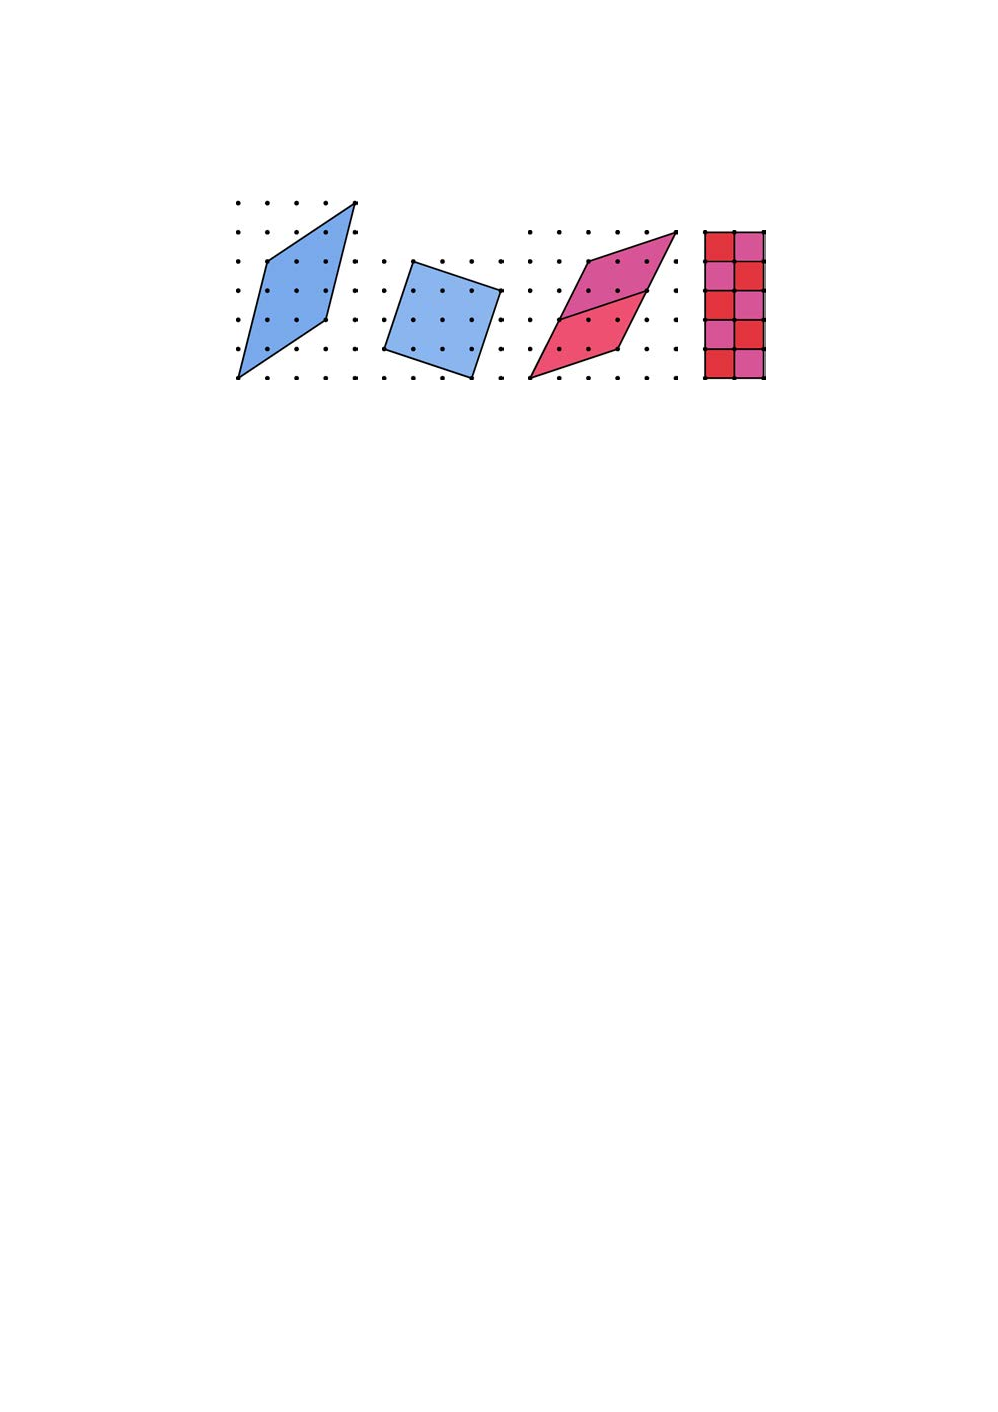
\includegraphics[width=0.60\textwidth]{Holmin15-Fig1}
  \caption{
Four Bravais cells of area 10, a figure from Holmin's PhD thesis\rf{Holmin15}.
The two blue Bravais cells are not
`primitive' (\ie, prime), as they are clearly
tiled by smaller prime Bravais cells.
Homlin claims that the two blue Bravais cells are
primitive, but that is wrong, see \refeq{Holmin15-Fig1HL}.
          }\label{Holmin15-Fig1}
\end{figure}

Wigman\rf{Wigman05}
{\em Counting singular matrices with primitive row vectors}: ``
Let us consider the set of singular $[n\times{n}]$ matrices with integer
entries. We are interested in the question how many among these matrices
have primitive row vectors, that is each row is not a nontrivial multiple
of an integer vector. We count the matrices according to the maximal
allowed Euclidean length of  the  rows.  Without  the  constraint  of
primitivity  the  problem  of  counting  such matrices  was  solved  by
Katznelson~[??].''

Wigman\rf{Wigman05} and Katznelson focus on asymptotic counting, which
we probably do not need.

\item[2020-02-19 Predrag]
Alexander Gorodnik
\HREF{https://www.math.uzh.ch/gorodnik/ds17/DynSysErgThPartI_17-18.pdf}
{lecture notes} discuss cat map $(A^n-\unit)$ and says
``The number of such solutions is exactly the area $\det(A^n-\unit)$ of
{\fundPip} in virtue of the

\textbf{Pick's theorem} (Gorodnik's Theorem 1.5.3, and A.4.1).
Let $i$ be the number of points with integer coordinates in the interior
of parallelogram $P$ and $b$ be the number of points with integer
coordinates on the perimeter of $P$. Then, Area$(P) =i+(b/2)+1$, with
points on the edges are counted as half and all vertices count as a
single point.

He proves the theorem. As usual, Pick's theorem is for $\reals^2$, not
general enough for us.

\item[2020-02-19 Predrag]
Baake, Hermisson and Pleasants\rf{BaHePl97}
{\em The torus parametrization of quasiperiodic {LI}-classes}
call this theorem a ``Fundamental  fact'' (their eq.~(10)), and
prove it, in Appendix for $d$\dmn\ tori maps, \ie,
in the case that we need. They use it to count all manner of tilings.
What they emphasize, and what we might have to
pay attention to, is the structure of the symmetry solutions on
$\mathbb{T}^d$.

\item[2020-02-21 Predrag]
Jezierski and Marzantowicz\rf{JezMar06}
\CBlibrary{JezMar06} write:

let $f:X \to X$ be a self-map of a set X.\\
(1.0.4) Definition. If $x \in X$ is a periodic point of f then any $m \in
N$ such that fm(x) = x is called a period of x. The smallest period of x
is called the minimal period of x with respect to f. The set of all
minimal periods of $x \in X$ is called the set of minimal periods of f
and denoted by Per(f).

We will define the fundamental algebraic invariants of a map f which
allow us to study the following notions:

\begin{itemize}
  \item Lefschetz number L(f) (cf. (2.3.12)), correspondingly Lefschetz numbers
{L(fm)} of all iterations and their algebraic combinations, informing about
the existence of fixed, respectively periodic points.
  \item Nielsen number N(f) (cf. (4.1.2)), correspondingly Nielsen periodic numbers
NFm(f) (cf. (5.1.16)), NPm(f) (cf. (5.1.14)) estimating from below
the number of fixed, respectively points of period m and m-periodic points.
\end{itemize}

[...]
This theory was initiated by Jakob Nielsen\rf{Nielsen1920} in 1920
% https://link.springer.com/content/pdf/10.1007/BF01457977.pdf
by the
observation that every self-map of the two-dimensional torus
$f:\mathbb{T}^2\to \mathbb{T}^2$  has at least |det(I-A)| fixed points
(here $I, A\in  M_{2{\times}2}(\integers)$ are respectively the identity
matrix and the matrix representing the induced homotopy homomorphism
$f_\#$ of $\pi_1(\mathbb{T}^2) = \integers^2$).

In 1975 R. Brooks, B. Brown J. Pak, and D. Taylor\rf{BBPT75}
derived a
nice formula for the Nielsen number $N(f)$ for the torus map: the Nielsen
number equals the absolute value of the Lefschetz number.
[...] The following theorem has been proved in \refref{BBPT75}.

(4.3.14) Theorem. For every self-map of the torus $f: \mathbb{T}^d \to
\mathbb{T}^d$, L(f) = det(I-A) and N(f) = |L(f)|.

Proof. Since the Lefschetz and Nielsen numbers are homotopy invariants we
may assume that $f = f_A$, i.e. f is induced by the linear map A.

\begin{enumerate}
  \item $f_A$ has exactly |det(I-A)| fixed points,
  \item no two fixed points of $f_A$ are Nielsen related,
  \item the index of each fixed point equals sgn(det(I-A)).
\end{enumerate}


[...] the fundamental theorem which allows us to extend the Nielsen fixed
point theory from tori into nilmanifolds. This theorem was proved
simultaneously by Anosov [An], and also Fadell and Husseini [FaHu2].

(6.3.13) Theorem. Let $f:X \to X$ be a self-map of a compact nilmanifold.
Then N(f) = |L(f)| and L(f) = det(I-A), where A denotes the
linearization matrix of f (cf. Definition (6.3.4), Proposition (6.3.6)).

\item[2020-02-22 Predrag]
Brooks \etal\rf{BBPT75}
{\em Nielsen numbers of maps of tori}:

If  $f:  X  \to X$  is  any  map on a $k$\dmn\ torus  X,  then the
Nielsen number and Lefschetz number of $f$  are  related by  the  formula
$N(f)=|L(f)|$.   Thus, on  the torus, the  Lefschetz number gives
information, not  just on  the existence of fixed points, but  on  the
number of  fixed points as  well. No  other compact Lie group has this
property.

\item[1995-09-08, 2020-12-08 Predrag]
Fel{'s}htyn and Hill\rf{FelHil95} {\em Trace formulae, {Zeta} functions,
congruences and {Reidemeister} torsion in {Nielsen} theory}
\arXiv{chao-dyn/9509009} paper is rich in examples of trace formulas and
zeta functions, but it's probably safe to ignore all this...

``
The Artin-Mazur zeta function and its modification count periodic points
of a map geometrically, the Lefschetz's type zeta functions do this
algebraically (with weight given by index theory). Another way to count the
periodic points is given by Nielsen theory.

The Lefschetz zeta function is always rational function of $z$ and is given by
a determinant formula. Manning\rf{manning} proved the rationality of the
Artin-Mazur zeta function for diffeomorphisms of a compact smooth manifold
satisfying Smale's Axiom A.

In Nielsen theory the `fixed point class' is determined by the `lifting
class'. A fixed point class is called \emph{essential} if its index is
nonzero. The number of lifting classes (and hence the number of fixed
point classes, empty or not) is called the \emph{Reidemeister Number}.
Generating functions for these numbers are called the Reidemeister zeta
and Nielsen zeta functions. They are homotopy invariants.
''

\end{description}


\subsection{Tensor eigenvalues}

In principle Han has solved the periodic states counting problem for
$d$\dmn\ hypercubic lattices by the discrete Fourier transform
diagonalization formula \refeq{HLreciprocal20}. A conceptual problem is
that the answer is stated in terms of $\cos$'s of rational angles, and it
is not obvious how those combine to yield an integer as the final result,
the number of periodic states.

For that reason it might be nice to perform the inverse Fourier transform
to the configuration space, to see what the basis vectors and the
fundamental parallelogram of the 2\dmn\ integer lattice look like, and
unify the treatment of the 1\dmn\ and higher\dmn\ lattice points
counting. We have looked at the relationship between the {\lattstate}s
and their Fourier representation in \refeq{FourierSpacePoints},
\reffig{fig:HLmtildeAndxtildeOf124Cycles},
\refeq{FourierCycPermT=4}, \etc.

Also we have some suggestive lattice solutions, such as
\refeq{HL2DimensionOrbit2}, \reffig{fig:HLAllPointsOf2By2Blocks}
(unit cube have been preferable - this is in the cube center coordiantes).

There is much literature on eigenvectors of tensors - probably we can
figure it out on our own, but I'm recording possible references just for
record here:

\begin{description}
\PCpost{2018-02-06}{
A job candidate Glen Evenbly talked about ``Tensor Networks'', (also
known as ``birdtracks'', but getting a citation out of computer nerds who
do it is harder than pulling teeth - at best I can pass under ``Penrose
diagrams''). If you want to see a lot of non-birdtracky pictures,
Rom{\'a}n Or{\'u}s \HREF{http://www.romanorus.com/DPGTutorial2014.pdf}
{has them}. Basically, if you are solving a 1D lattice problem, the
transfer operator is a matrix. However, if you are acting on a 2{\dmn} or
higher lattice, the transfer operator has pairs of more indices replacing
each index ow the 1D matrix, hence ``tensor.'' We need to understand that
as we go from cat map Toeplitz matrices to their $d$\dmn\
generalizations.
    }


\item[2020-02-14 Predrag]
Mateusz Micha{\l}ek and Bernd Sturmfels\rf{MicStu20}
{\em Invitation to Nonlinear Algebra},  \CBlibrary{MicStu20}
discuss symmetric $[n\!\times\!n]$ matrices tensor eigenvectors in Sect.~9.1.

The main monograph in this subject is
Qi, Chen and Chen\rf{QiChCh18}
{\em Tensor Eigenvalues and Their Applications},  \CBlibrary{QiChCh18}.

They find convenient to replace the n\dmn\ affine space  with the
(n-1)\dmn\ projective space, where two nonzero vectors are identified if
they are parallel.

Papers not looked at yet:

{\em All Real Eigenvalues of Symmetric Tensors}
\HREF{https://doi.org/10.1137/140962292} {DOI}:

{\em Generalized Tensor Eigenvalue Problems}
\HREF{https://doi.org/10.1137/140975656} {DOI}:

 {\em On determinants and eigenvalue theory of tensors}
\HREF{https://doi.org/10.1016/j.jsc.2012.10.001} {DOI}:

%{\em ##}
%\HREF{##} {DOI}:

%{\em ##}
%\HREF{##} {DOI}:

%\HREF{} {wiki}:

%\HREF{} {wiki}:


\end{description}


\section{Difference equations}
\label{sect:diffEqs}

\subsubsection*{sect.~2.3
                Linear homogenous equations with constant coefficients,
                Elaydi\rf{Elaydi05}}
% 2020-03-28 Predrag

Consider \emph{$k$th-order difference equation}
\beq
\field_{n+k} + p_1\,\field_{n+k-1} + p_2\,\field_{n+k-2}
             + \cdots + p_k\,\field_{n} = 0
\,,
\ee{Elaydi05(2.3.1)}
where $p_i$ are constants and $p_k\neq0$.
A $k$th-order difference equation with constant coefficients is often
referred to as $(k+1)$-term recurrence relation, see
\refsect{sect:genFuncts}.
Assuming a solution of form
$\field_{n}=\ExpaEig^n$ leads to the \emph{characteristic equation}
(see also `characteristic function' \refeq{FGHLW74:charFunct1d})
\beq
\ExpaEig^{k} + p_1\ExpaEig^{k-1} + p_2\ExpaEig^{k-2}
             + \cdots + p_k = 0
\,,
\ee{Elaydi05(2.3.2)}
with characteristic roots
\(
\{\ExpaEig_{1},\ExpaEig_{2},\cdots,\ExpaEig_{k}\}
\,.
\)
If the roots are distinct,
\[
\{\ExpaEig_{1}^\cl{},\ExpaEig_{2}^\cl{},\cdots,\ExpaEig_{k}^\cl{}\}
\]
is a set of fundamental solutions, and the general solution is of form
\beq
\field_{\cl{}}  = \sum_{i=1}^{k} a_i\ExpaEig_{i}^\cl{}
\,,
\label{Elaydi05(2.3.4)}
\eeq
where constants $a_i$ are determined by the initial conditions
$\{\field_{0},\field_{1},\cdots,\field_{k-1}\}$.


If the roots are not distinct, one also has fundamental solutions
of form $\cl{}^m\ExpaEig_{i}^\cl{}$.

\subsubsection*{sect.~2.4
                Linear inhomogenous equations,
                Elaydi\rf{Elaydi05}}
% 2020-03-28 Predrag

\beq
\field_{n+k} + p_1\,\field_{n+k-1} + p_2\,\field_{n+k-2}
             + \cdots + p_k\,\field_{n} = g_{n}
%\,,
\ee{Elaydi05(2.4.4)}
represents a physical system in which the \emph{forcing term}
(or \emph{external force}, or \emph{control}, or \emph{input}) $g_{n}$
is the input, and $\field_{n}$ the output,
\[
g_{n} \to \mbox{ system } \to \field_{n}
\,.
\]
The solutions of \refeq{Elaydi05(2.4.4)} do not form a vector space, \ie,
their linear combinations are not also solutions. However, a difference
of any pair of solutions is a solution of the homogenous difference
equation \refeq{Elaydi05(2.3.1)}, and a general solution of the linear
inhomogenous system \refeq{Elaydi05(2.4.4)} is a sum of the
\emph{complementary} solution (a homogenous solution $\field_{c}$ of
\refeq{Elaydi05(2.3.1)}, and a \emph{particular} solution $\field_{p}$
\beq
\field_{n} = \field_{c,n} + \field_{p,n}
%\,,
\ee{Elaydi05(2.4.3)}
A simple example of a particular solution: if $g_{n}=a^n$, then
$\field_{p,n}=c_1a^n$.

\bigskip

\begin{description}
\item[2020-03-28 Predrag]
There are many books on difference equations. \\
I like
Elaydi\rf{Elaydi05} \CBlibrary{Elaydi05}, but I have also downloaded\\
% Woods\rf{Woods12}
% {\em Multidimensional signal, image, and video processing and coding}
% \HREF{http://ChaosBook.org/library/Woods12} { (click here)}\\
Kelley and Peterson\rf{KelPet01} \CBlibrary{KelPet01}\\
Agarwal\rf{Agarwal00} \CBlibrary{Agarwal00}\\
Agarwal\rf{Agarwal06} \CBlibrary{Agarwal06}\\
Allen, Aulbach, Elaydi and Sacker\rf{AAES05} \CBlibrary{AAES05}\\
Galor\rf{Galor07} \CBlibrary{Galor07}\\
Ozisik, Orlande, Colaco and Cotta\rf{OOCC17} \CBlibrary{OOCC17}\\
Micciancio and Goldwasser\rf{MicG0l02}\\
% {\em Complexity of Lattice Problems - A Cryptographic Perspective}

\item[2020-04-13 Predrag]
Dannan, Elaydi and Liu\rf{DaElLi00}
{\em Periodic solutions of difference equations}
is a treasure trove of results on periodic solutions of difference equations:
marginal eigenvalues, Floquet exponents and multipliers,
Fredholm alternative.

    \item[2020-08-10 Predrag]
Lick\rf{Lick89} {\em Difference Equations from Differential Equations}
\CBlibrary{Lick89} we probably do not need.

The most general, quasi-linear, second-order PDE in two independent
variables is his eq.~(2.0.2). Depending on coefficients, the equation can
be \emph{hyperbolic}, such as the $d=2$ spacetime wave equation (2.0.3).
He focuses on \emph{parabolic} (${s}=2$ for us), such as the time
dependent diffusion equation given by (2.0.4).

Elliptic equations usually describe the steady-state limit of problems
where the time-dependent problem is described by parabolic or hyperbolic
partial differential equations. The most common elliptic equation is
$d=2$ space`time' symmetric Laplace's equation (2.0.5).

He defines Helmholtz equation (4.0.5),
 Laplace's equation (4.0.6), and Poisson's equation (4.0.7).
 His emphasis is on the discretized Helmholtz equation (4.1.3).

Sect.~2.4 {\em Algorithms for Two-Dimensional Problems}
has the 5-term recurrence, his eq.~(2.4.3) and (4.1.3).

Difference equations arising from elliptic equations generally
necessitate the solution of a large set of linear algebraic equations.
The matrix corresponding to this set of equations is generally sparse and
good solution methods take advantage of this fact.
[...]
the direct solution of these difference equations is quite time
consuming. When the number of equations is large, iterative methods of
solution are usually more efficient.

(4.2.8) defines \emph{Jacobi iteration}, a method of improving initial
guess solution.
(4.2.9) method is known as Gauss-Seidel iteration or the method of
successive relaxation.



\item[2016-07-11 Predrag]
%\subsection{Martin / Martin06}\label{sect:Martin06}
Boris cites P. A. Martin\rf{Martin06} {\em Discrete scattering theory: {Green}'s
function for a square lattice}

The \emph{lattice Green's function} is the main subject of the paper.

We consider the simplest problem, with a two-dimensional, square lattice.
Each lattice point can move out of the plane of the lattice, and that each
point is connected to its neighbours by springs; only nearest-neighbour
interactions are included. This leads to a system of partial difference
equations. The same equations are obtained if the two-dimensional Helmholtz
equation is discretized using the central-difference approximation (lattice
d'Alembert operator) for the Laplacian.

\item[2017-09-11 Predrag]
Morita\rf{Morita71} {\em Useful procedure for computing the lattice
{Green's} function - square, tetragonal, and bcc lattices}: `` A
recurrence relation, which gives the values of the lattice Green's
function along the diagonal direction from a couple of the elliptic
integrals of the first \refeq{Cserti00(38)} and second kind, is derived
for the square lattice by an elementary partial integration. The values
of the square lattice Green's function at an arbitrary site are then
calculated in a successive way with the aid of the difference equation
defining the function.
''
The method yields a recursion formula for a peculiar lattice Green's function
on a 2d lattice, but not the LGF itself.


\item[2017-09-09 Predrag]
Simons\rf{Simons97}
uses \refeq{Elaydi05(2.3.4)} in his \refeq{YamAbd97fundSol} to
invert a particular banded matrix.

See also \refexam{exam:TentLCod}~{\em Tent map linear code.}

Compare {characteristic equation} \refeq{Elaydi05(2.3.2)} to the
characteristic function $a(z)$ \refeq{FGHLW74:charFunct1d}.

\end{description}

\subsection{Time quasilattices}
\label{sect:timeQuasiLatt}

{\bf 2018-10-10, 2020-03-12 Predrag} Felix Flicker writes:
``My student Leon Zaporski and I have been investigating the
topological entropy of substitution sequences in the symbolic dynamics of
periodic orbits in discrete-time dynamical systems. We were hoping you
might be willing to take a look at our draft,
Zaporski and Flicker\rf{ZapFli19} {\em Superconvergence of topological
entropy in the symbolic dynamics of substitution sequences},
\arXiv{1811.00331},
and to send any
thoughts you might have, both in terms of whether you think the results
would be of interest to the community, and if there is a journal you
might recommend for us to submit to.''
\begin{quote}
                                        \toCB
I failed to read it. But it needs to be included in ChaosBook, as well
as many of the references.
\end{quote}
Their Fig.~1 is the topological entropy as a function of a control
parameter of the logistic map\rf{PeCaCe94}.
[...]
In the cases that accumulation points correspond to generalised time
quasilattices, the Boyle-Steinhardt class\rf{BoySte16} is indicated above
the curve.
\begin{quote}
Predrag:
I made several attempts to get some kind
of renormalization theory for the Sharkovsky sequence, with no
interesting results to report. Dahlquist wrote up his attempt
\toChaosBook{section.R.1} {(click here)}.
\end{quote}
[...]
Period doubling continues to be of importance to cutting edge research:
recent experiments established the existence of (discrete) time crystals,
which spontaneously break the symmetry of a periodic driving by returning
a robust period-doubled response, made rigid to perturbations and finite
temperature by the local interactions of many degrees of freedom.
[...]
periodically-driven nonlinear systems can feature not just period-doubled
responses, but robust responses with the symmetries of one-dimensional
(generalised) \emph{time quasilattices}\rf{Flicker18}.
[...]
Quasilattice substitution rules fall within the set we consider, and, by
considering a simple generalisation of the basic quasilattice concept, we
find that we are able to identify aperiodic orbits corresponding to all
physically relevant quasilattices, extending previous results identifying
two cases. Generalizing further we consider a set of substitutions
additionally covering, for example, the period-doubling cascade.
[...]
Whereas the topological entropy is zero for all sequences in the
period-doubling cascade, for other substitution sequences it increases
monotonically.
[...]
We find that the topological entropy of the wide class of substitution
sequences we consider converges as a double exponential onto its
accumulation point.
[...]
We demonstrate that all one-dimensional quasilattices can appear as
stable orbits in nonlinear dynamical systems.

Here is something we might find useful for \catlatt:

[...]
we focus on the \emph{generalised composition rules}, which systematically
generate admissible words by a substitution process\rf{Bruijn81}.

[...]
The universal order of periodic windows coincides with the
\emph{parity-lexicographic order} of words, defined through the relation
`$\prec$' in the following way:
\[
L \prec C \prec R
\]
and for two admissible words they state it in a way that is perhaps
superior to                                         \toCB
\toChaosBook{section.14.5}{ChaosBook}. Cite it there.
\medskip

[...]
{\bf Word operations}
\begin{itemize}
\item $\bar{\mathbf{A}} \bar{\mathbf{B}}$ indicates the concatenation of words $\bar{\mathbf{A}}$ and $\bar{\mathbf{B}}$
\item $\lvert\bar{\mathbf{A}}\rvert$ returns the number of letters in $\bar{\mathbf{A}}$
\item $\lvert\bar{\mathbf{A}}\rvert_{R,L}$ returns the number of letters $R,L$ in $\bar{\mathbf{A}}$
\item $\bar{\mathbf{A}}\rvert_C$ substitutes the final letter of $\bar{\mathbf{A}}$ with the letter $C$.
\end{itemize}
%
Inverse words are defined as follows (Predrag - I do not understand this):
%
\begin{align}
\bar{\mathbf{A}}^{-1}\left(\bar{\mathbf{A}}\bar{\mathbf{B}}\right)=\bar{\mathbf{B}}\nonumber\\
\left(\bar{\mathbf{A}}\bar{\mathbf{B}}\right)\bar{\mathbf{B}}^{-1}=\bar{\mathbf{A}}.
\end{align}

\begin{theorem}\label{secorder} %
Substitution rules generating a cascade
with initial word $\bar{\mathbf{W}}_{1}=R$ and
$\bar{\mathbf{W}}_{2}=\bar{\mathbf{R}}$ can be restated as a second order
linear recursive relation
$\bar{\mathbf{W}}_{n+2}=g(\bar{\mathbf{W}}_{n},\bar{\mathbf{W}}_{n+1})$
under concatenation if
$\bar{\mathbf{W}}_{3}=g(\bar{\mathbf{W}}_{1},\bar{\mathbf{W}}_{2})$. %
\end{theorem}
[...]
Consider a $[2\times2]$ \emph{growth matrix}
\begin{align}
A=\left(\begin{array}{cc}
a & b\\
c & d
\end{array}\right)
\end{align}
which quantifies the growth in the numbers of each letter type:
\begin{align}
\left(\begin{array}{c}
\left|\bar{\mathbf{W}}_{n}\right|_R\\
\left|\bar{\mathbf{W}}_{n}\right|_L
\end{array}\right)\rightarrow\left(\begin{array}{cc}
a & b\\
c & d
\end{array}\right)\left(\begin{array}{c}
\left|\bar{\mathbf{W}}_n\right|_R\\
\left|\bar{\mathbf{W}}_n\right|_L
\end{array}\right)=\left(\begin{array}{c}
\left|\bar{\mathbf{W}}_{n+1}\right|_R\\
\left|\bar{\mathbf{W}}_{n+1}\right|_L
\end{array}\right)
\end{align}
The class of substitutions we consider
can then be written as
%
\begin{align}
\bar{\mathbf{W}}_{n}&=\bar{\mathbf{W}}_{n-1}\mathcal{P}\left(\bar{\mathbf{W}}_{n-1}^{\text{tr}\left(A\right)-1}\bar{\mathbf{W}}_{n-2}^{-\det\left(A\right)}\right)
\end{align}
%
for $n>2$, with $\bar{\mathbf{W}}_{1}=R$, and $\bar{\mathbf{W}}_{2}$
a specified word. The symbol $\mathcal{P}$ indicates an unspecified
permutation. The characteristic equation of the growth matrix $A$ is
%
\begin{align}
\lambda^{2}-\text{tr}\left(A\right)\lambda+\det\left(A\right)&=0
\,.
\label{eq:W_characteristic}
\end{align}
%
The eigenvalues of $A$  must be real, either integer or quadratic irrational
(when we consider quasilattices).
The ratio of the components of the eigenvector associated to the largest
eigenvalue gives the relative frequencies of the two cell
types\rf{BoySte16}.
Eq.~\eqref{eq:W_characteristic} can be seen as the $n\rightarrow\infty$
limit of the defining equation of some integer sequence $W_n$ given by
%
\begin{align}
W_{n}&=\text{tr}\left(A\right)W_{n-1}-\det\left(A\right)W_{n-2}
\end{align}
for $n>2$, $W_1=\left|\bar{\mathbf{W}}_1\right|=1$, and
$W_2=\left|\bar{\mathbf{W}}_2\right|$. The ratio $W_n/W_{n-1}$ gives the
best possible rational approximation, for denominators not larger than
$W_{n-1}$, to the largest eigenvalue of the growth matrix, \emph{i.e.}
the larger of the solutions to Eq.~\eqref{eq:W_characteristic}.

[...]
As an example, the period-doubling substitutions lead to
the integer sequence
%
\begin{align}
W_n=W_{n-1}+2W_{n-2}
\end{align}
%
for $n>2$, with $W_1=\left|\bar{\mathbf{W}}_1\right|=\left|R\right|=1$ and $W_2=\left|\bar{\mathbf{W}}_2\right|=\left|RL\right|=2$. Explicitly, the first few terms are
%
\begin{align}
1,\,2,\,4,\,8,\,16,\,32,\,64,\ldots
\end{align}
%
\emph{i.e.} $W_n=2^{n-1}$.
\begin{quote}
Predrag: This is perhaps related to $s=2$ version of
\refeq{Chen11:1stepDiffSolu}.
\end{quote}
Then they do Fibonacci.
[...]
The eigenvalues of a $[2\times2]$ growth matrix $A$ are real and given by
%
\begin{align}
\lambda_\pm=
\frac{1}{2}\left({s}\pm\sqrt{{s}^2-4\det{A}}\right)
\,,\quad
{s}=\tr{A}
\,.
\label{eq:characteristic}
\end{align}
%
If ${s}^2=4\det{A}$ they are integers. Otherwise,
the larger eigenvalue is a quadratic irrational `Pisot-Vijayaraghavan'
(PV) number: the largest root of an irreducible monic polynomial, all of
whose Galois conjugates have modulus strictly less than
one.
[...]
The three conditions are necessary and sufficient for the
substitutions to correspond to quasilattice inflation
rules\rf{BoySte16}:
\begin{enumerate}
\item the growth matrix must be unimodular, $\left|\det{A}\right|=1$
\item there must be two spacings between each symbol
\item the largest eigenvalue of the growth matrix must be a PV number.
\end{enumerate}
The condition $\left|\det{A}\right|=1$, implies the inverse of the growth
matrix is also an integer matrix. The
inflation (substitution) of any quasilattice sequence can therefore be
undone with a well-defined deflation. This endows quasilattices with a
discrete scale invariance\rf{BoDiFl20}.
The third, PV numbers condition is necessary for the
interpretation of the quasilattice sequence in terms of a cut through a
higher-dimensional regular lattice.

The concept of quasilattices
relating to higher-dimensional lattices is discussed at length in
\refrefs{BoySte16,Flicker18}. % ,FlickervanWezel15}.

\begin{quote}
Predrag: So our ${s}=3$ \templatt\ $\lambda^{2}-3\lambda+1=0$ eigenvalue
$\frac{3+\sqrt{5}}{2}$ turns out to be a PV number. So is
${s}=4$ \templatt\ $\lambda^{2}-4\lambda+1=0$ eigenvalue
$2+\sqrt{3}$.
Both are the Boyle-Steinhardt\rf{BoySte16} quasilattices, of class 1,
respectively 3.
\end{quote}
[...]
Starting from an orbit described by the word $R$, repeated application of
the inflation rules will lead to a cascade of stable periodic orbits of
increasing length. After an infinite number of substitutions, \emph{i.e.}
at the accumulation point of the sequence, lies a stable orbit described
by an aperiodic word: a \emph{time quasilattice}.
[...]
Characteristic equation
%
\begin{align}
\lambda^2=4\lambda-1.
\end{align}
leads to the (modulus of the)
Clapeyron numbers $C_n$ ($A125905$ in the
\HREF{https://oeis.org/} {On-Line Encyclopedia} of
Integer Sequences)
\begin{align}
C_n=4C_{n-1}-C_{n-2}
\end{align}
for $n>2$ with $C_1=1$, $C_2=4$.
\begin{quote}
Predrag: In conclusion, \templatt\ is related to counting
of quasilattice words. Not sure it is of any use to us.
\end{quote}


\begin{description}

\item[2020-04-12 Predrag] Have a look at
Flicker, Simon and Parameswaran\rf{FlSiPa20}
{\em Classical dimers on {Penrose} tilings}.
[...]
[...]
[...]
[...]
[...]
[...]
[...]
[...]
[...]

\end{description}



\section{Generating functions}
\label{sect:genFuncts}

(Note, there is also a totally unrelated Lagrangian `generating function',
\refsect{sect:GenFuncLit}, nothing to do with this section of the blog.)
\bigskip

{\bf Definition}\rf{BecRob07}.
Let $f(x)$ be a series in powers of $x$. Then by the
symbol $[x^n]f(x)$ we will mean the coefficient of $x^n$ in the series
$f(x)$.



\begin{description}

\item[2020-03-20 Predrag]                               \toCB
The theory generating function (AKA Z-transforms) is pedagogically
explained by Elaydi\rf{Elaydi05}, including a table of common
Z-transform pairs, in analogy with the familiar Laplace transform tables.

\item[2020-09-30 Predrag]                               \toCB
Online
\HREF{http://pilot.cnxproject.org/content/collection/col10064/latest/}
{Signals and Systems} has pedagogical chapters on Z-transforms.

\item[2020-07-11 Predrag]
Woods\rf{Woods12}
{\em Multidimensional signal, image, and video processing and coding},
Chap.~3 {\em Two-Dimensional Systems and Z-Transforms}
 (2012) \CBlibrary{Woods12}.

\item[2020-01-23 Predrag]
For multivariate
generating functions
\beq
N(z)\,,\qquad
z^n=z^{n_1}z^{n_2}\cdots{z^{n_d}}
\,,
\ee{genFuncts:multiVar}
see
\refeq{coneKgenF},
\refeq{BecRob07:LaurMon},
\refeq{BecRob07:IntPoTrnsf},
\refeq{BecRob07:examp3-4}
.

Other examples of generating functions:
\refeq{2ndChebGenF},
\refeq{Wu04:gen},
\refeq{eq:DetPfaffianRel}
.

\item[2020-04-07 Han]
\renewcommand\speriod[1]{{\ensuremath{L_{#1}}}}  %continuous spatial period
\renewcommand\period[1]{{\ensuremath{T_{#1}}}}  %continuous time period
Perhaps we need three generating function variables
\bea
N(z_1,z_2,z_3)
    & = &
\sum_{\speriod{}=1} N_{\BravCell{\speriod{}}{\period{}}{\tilt{}}}
   z_1^{\speriod{}}z_2^{\period{}} z_3^{\tilt{}}
%    \continue
%    \ceq
\,.,
\label{3varPerOrCount}
\eea
Here $z_3^{\tilt{}}$ sum is finite, $-\speriod{}<{\tilt{}}<\speriod{}$,
and that feels not sufficiently invariant, as it depends on Hermite normal form
convention. Need something invariant...
\renewcommand\speriod[1]{{\ensuremath{\ell_{#1}}}}  %continuous spatial period
\renewcommand\period[1]{{\ensuremath{\ell_{#1}}}}  %continuous time period

\item[2020-03-01 Predrag]
Cute but true; Wilf\rf{Wilf94} {\em Generatingfunctionology} defines
the periodic points counting generating function as
\beq
N(z) = \sum_{\cl{}\geq0} N_n z^n
\,,
\ee{Wilf94:genFunct}
and starts out in his sect. 1.1~{\em An easy 2-term recurrence}, with
our Bernoulli periodic points count (for the ${s}=2$ case only)
\beq
N_{\cl{}} = s^{\cl{}} - 1
\,,
\ee{genFuncts:noPerPtsBm}
as a trivial example of a two-term recurrence (first-order difference
equation\rf{Elaydi05})
\beq
N_{\cl{}+1} = 2\,N_{\cl{}} + 1 \,,\qquad (s=2;\cl{}\geq0, N_0=0)
\,,
\ee{Wilf94:noPerPtsBm}
and (Predrag's insert) for  ${s}\neq2$,
\beq
N_{\cl{}+1} - s\,N_{\cl{}} = (s-1) \,,\qquad (\cl{}\geq0, N_0=0)
\,,
\ee{genFuncts:noPerPtsBms}
and its conversion to the periodic points count generating function
\refeq{Wilf94:genFunct}.
For \refeq{Wilf94:noPerPtsBm} he derives and expands in partial fractions
\beq
N(z;2) = \frac{z}{(1-z)(1-2z)} =  \frac{2z}{1-2z} -  \frac{z}{1-z}
\,,
\ee{Wilf94:noPerPtsGF}
and (Predrag's addition) for ${s}\neq1$,
\beq
N(z;s) = ({s}-1)z + ({s}-1)({s}+1)z^2 + ({s}-1)({s}^2+{s}+1)z^3 + \cdots
\,,
\ee{Wilf94:noPerPtsGFs}
verifying the Bernoulli periodic points count
\refeq{genFuncts:noPerPtsBm}.
Take
\(
N_{\cl{}} = ({s}-1)\hat{N}_{\cl{}}
\,,
\)
then \refeq{genFuncts:noPerPtsBms} leads to
\beq
\hat{N}_{\cl{}+1}  -{s}\,\hat{N}_{\cl{}} = 1
 \,,\qquad
(\cl{}\geq0, \hat{N}_0=0, \hat{N}_1 = 1)
\,.
\ee{genFuncts:BernRec-s1}
\beq
\hat{N}(z;s) = z + ({s}+1)z^2 + ({s}^2+{s}+1)z^3 + \cdots
\,,
\ee{Wilf94:noPerPtsGFs1}
For $s=1$ this is a complicated way to generate integers.


Then he does, as an example of a 3-term recurrence
(second-order difference equation\rf{Elaydi05}),
the Fibonacci recurrence
\beq
F_{n+1} = F_{n}+F_{n-1}:  \,,\qquad (\cl{}\geq1, F_0=0, F_1 = 1)
\,,
\ee{Wilf94:FibRec}
and derives
\beq
N(z) = \frac{z}{1-z-z^2}
     =
\frac{1}{z^{-1}-1-z}
\,.
\ee{Wilf94:FibRecGF}
Here the expansion in partial fractions is
in terms of roots of the (`golden mean') polynomial
\(
1-z-z^2
\)
.

He notes that the Stirling numbers of the first kind satisfy a 3-term
recurrence relation.


\item[2020-06-20 Predrag]
Oscar Levin %\rf{Levin19}
{\em Discrete Mathematics: An Open Introduction}
\HREF{http://discrete.openmathbooks.org/dmoi3/sec_addtops-genfun.html}
{Sect.~5.1 Generating Functions} works out a 3-term recurrence
$a_n = 3a_{n-1} - 2a_{n-2}$, with $a_0=1,a_1=3$ in
Example 5.1.6.  Surprisingly, one gets again (!)
\[
a_n = 2^{n+1} - 1
\,.
\]

\item[2020-06-20 Predrag]
Check out also Al Doerr and Ken Levasseur
\HREF{http://faculty.uml.edu/klevasseur/ads/index-ads.html}
{{\em Applied Discrete Structures}}:

\HREF{http://faculty.uml.edu/klevasseur/ads/s-recurrence-relations.html}
{{\em Sect.~8.3 Recurrence relations}}.

\HREF{http://faculty.uml.edu/klevasseur/ads/s-generating-functions.html}
{{\em Sect.~8.5.2 Solution of a Recurrence Relation Using Generating Functions}}.

\item[2020-03-04 Predrag]
\HREF{http://www.maths.surrey.ac.uk/hosted-sites/R.Knott/Fibonacci/LRGF.html\#section2.1}
{Ron Knott} writes:

The series of natural numbers
$1, 2, 3, 4, \cdots$
has the generating function
\beq
\frac{1}{(1-z)^2}=\frac{1}{1-2z+z^2}
\ee{genFuncts:n}
and the 3-term  recurrence (second-order difference equation\rf{Elaydi05})
%\[
%\field_{n}=2\field_{n-1}-\field_{n-2}
%\]
%We can see the relationship more clearly if we rewrite the recurrence in this form:
\[
\field_{n}-2\field_{n-1}+\field_{n-2}=0
\]
and compare that with the denominator of the generating function, namely:
\[
1-2z+z^2
\]
which might be a way to understand why $s=2$ is special.

A variant of Fibonnaci:
0,1,3,8,21,...is generated by
\[
\frac{z}{z^2-3z+1}
=
\frac{1}{z-3+z^{-1}}
\]
which looks \templatt-like.

\item[2020-03-02 Predrag]
In sect.~1.4 {\em A three term boundary value problem} Wilf\rf{Wilf94}
considers a 3-term recurrence with Dirichlet \bcs
\beq
au_{n+1} + bu_{n} + cu_{n-1} = d_{n} \,,\qquad
(n = 1,2,...,N-1;u_0 = u_N = 0)
\ee{Wilf94(1.4.1)}
where the positive integer N, the constants a, b, c and the sequence
$\{d_n\}^{N-1}_{n=1}$ are given in advance. The eqs \refeq{Wilf94(1.4.1)}
determine the sequence $\{u_i\}^N_0$ uniquely. Such boundary value
problems arise in applications such as the interpolation by spline
functions.

\bigskip

\item[2020-03-01 Predrag]
Compare \refeq{genFuncts:noPerPtsBms} to our\rf{CL18} Bernoulli 1-step difference
condition
\beq
\field_{\zeit} - {s}\field_{\zeit-1} = - \Ssym{\zeit}
\,,\qquad  \field_{\zeit} \in [0,1)
\,.
\ee{genFuncts:1stepDiffEq}
This suggests that the periodic points count is obtained by
\beq
\field_{\zeit} \to N_\cl{}\,,  \Ssym{\zeit} \to 1-{s}
\,.
\ee{genFuncts:interp}

The \templatt\ second-order difference equation is
\beq
\field_{\zeit+1}  -  s \, \field_{\zeit} + \field_{\zeit-1}
    =
-\Ssym{\zeit}
\,,
\ee{genFuncts:CatMapNewt}
Mimicking \refeq{genFuncts:interp}, my guess for the recurrence for
periodic points count is
\beq
N_{\cl{}+1}  -{s}\,N_{\cl{}} +N_{\cl{}-1}   = 2(s-2)
 \,,\qquad
(\cl{}\geq1, N_0=0, N_1 = s-2)
\,.
\ee{genFuncts:CatRec-s}
\beq
N_{\cl{}+1}  -({\mu}^2+2)\,N_{\cl{}} +N_{\cl{}-1}   = 2{\mu}^2
 \,,\qquad
(\cl{}\geq1, N_0=0, N_1 = {\mu}^2)
\,.
\ee{genFuncts:CatRec-mu}
Indeed, this generates the correct series for arbitrary $s$
(compare with \refeq{PC:1stepDiffSolu},
\refeq{JacOperCount}.)
\bea
N(z;s) &=& ({s}-2)z + (s-2)({s}+2)z^2 + ({s}-2)({s}+1)^2z^3
    \ceq
 + ({s}-2)({s}+2)\,{s}^2 z^4
 +
\label{genFuncts:CatMapN-s}
\eea
\bea
N(z:{\mu}^2) &=& {\mu}^2z + {\mu}^2({\mu}^2+4)z^2 + {\mu}^2({\mu}^2+3)^2z^3
    \ceq
 + {\mu}^2({\mu}^2+4)\,({\mu}^2+2)^2 z^4
 +
\label{genFuncts:CatMapN-mu}
\eea
Take
\(
N_{\cl{}} = {\mu}^2\hat{N}_{\cl{}}
\,,
\)
then \refeq{genFuncts:CatRec-s} leads to
\beq
\hat{N}_{\cl{}+1}  -{s}\,\hat{N}_{\cl{}} +\hat{N}_{\cl{}-1}   = 2
 \,,\qquad
(\cl{}\geq1, \hat{N}_0=0, \hat{N}_1 = 1)
\,.
\ee{genFuncts:CatRec-s1}
\bea
\hat{N}(z;s) &=& z + ({s}+2)z^2 + ({s}+1)^2 z^3 + ({s}+2)\,{s}^2 z^4
    \ceq
 + (s^2+ s-1)^2z^5
 + (s^2-1)^2(s+2) z^6
 +
\label{genFuncts:CatMapN-s1}
\eea
\bea
\hat{N}(z;s) &=& z + ({\mu}^2+4)z^2 + ({\mu}^2+3)^2z^3 + ({\mu}^2+4)\,({\mu}^2+2)^2 z^4
    \ceq
 + ({\mu}^4+3\,{\mu}^2+5)^2 z^5
 + ({\mu}^2+1)^2({\mu}^2+3)^2({\mu}^2+4)z^6
 +
\label{genF:CatMapN-mu}
\eea
For ${\mu}=0$ this is a complicated way to generate integers squared
(see also \refeq{genFuncts:n})
\bea
\hat{N}(z;2) &=& z + 4z^2 + 9z^3 + 16 z^4 + 25 z^5 + 36 z^6 +
\label{genFuncts:CatMapN-s2}
\eea
Recurrence \refeq{genFuncts:CatMapN-s} appears correct for the $s=3$
count (have not rechecked)
\bea
N(z;3)
    &=&
 z+5 z^2+16 z^3+45 z^4+121 z^5+320 z^6+841 z^7
    \ceq
+2205 z^8+5776 z^9+15125 z^{10}
+39601 z^{11}
+\cdots
\,.
\label{genFuncts:catMapN_n-s=3}
\eea

\item[2020-03-02 Predrag]
In sect.~1.5 {\em Two independent variables} and
1.6~{\em Another 2-variable case} Wilf\rf{Wilf94}
considers problems that involve functions of two discrete variables.
His example is combinatorial, probably not what we need.

A generating function with the $1/n!$'s thrown into the coefficients, is
called an \emph{exponential generating function}. After his eq.~(1.6.12),
he explains the
\[
   x(d/dx)\log
\]
operation. He works it out for the ``Bell numbers', and derives that
the Bell numbers satisfy the recurrence depending on all previous Bell
numbers, much like the ChaosBook formulas for cumulants.

He says, comfortingly: ``[...]  there's no need for the guilt, because
the various manipulations can be carried out in the ring of formal power
series, where questions of convergence are nonexistent.''

\item[2012-06-19 Predrag]
In \toChaosBook{section.18.8} {example} 18.12 (edition 16.4.5), I show
that for alphabet
\(
    \A=\{a,cb^k; \,\, \overline{b}\}
\)
, the cycle counting {$\zeta$}-function is
\[
\zetatop = 1-3z+z^2
\,,
\]
\ie, the Isola\rf{Isola90} {$\zeta$}-function
\refeq{Isola90-13b}
for
$s=3$, without the $(1 - z)^2$ factor
(see \refeq{Isola90-13},
\refeq{Isola90-13c},
\refeq{AABHM99-46},
\refeq{Ising:Isola90-13}). That might be a simple
statement of the cat map symbolic dynamics.


\item[2020-02-09 Predrag]
Fischer, Golub, Hald, Leiva and Widlund\rf{FGHLW74}
{\em On {Fourier-Toeplitz} methods for separable elliptic problems}
solve linear equations, where $M$ arises from a finite difference
approximation to an elliptic partial differential equation.

Such a situation arises for those problems that can be handled by the
classical separation-of-variables technique. Their methods
are a computer implementation of the
separation of variables carried out on a discretized model of the
elliptic differential equation.

In one\dmn\ lattice, the \emph{characteristic function} $a(\ssp)$ of a symmetric
2$k$-banded Toeplitz matrix $A$ is defined as
\beq
a(\ssp) = a_k\ssp^k +\cdots+ a_0 +\cdots+ a_k\ssp^{-k}
%\,.
\ee{FGHLW74:charFunct1d}
(see \refeq{3diagToeplitz}, for example).
Such matrices occur in
fourth, or higher, order accurate finite difference approximation to second order
elliptic problems, when solving the bi-harmonic problem by a Fourier method, in
higher order spline interpolation, etc.

For a 1\dmn\ lattice one assumes that the characteristic function
$a(\ssp)$ has no roots on the unit circle. Then they factor
$a(\ssp)=\ell(\ssp)\,\ell(l/\ssp)$, where $l(\ssp)=b_0+\cdots+b_k\ssp^k$,
$b_0 > 0$, is a real polynomial with no roots inside the unit circle,
their Lemma 1. The factors $\ell(\ssp)$ and $\ell(l/\ssp)$ of $a(\ssp)$
are known as the \emph{Hurwitz factors}. Predrag has not found any useful
literature on these.

Their algorithm applied to the \templatt\ tri-diagonal case
\refeq{3diagCirculant} with $a_1=-1$ and $a_0 > 2$, has
linear convergence; see obscure references
\\
{[3]} F. L. Bauer, "Ein direktes Iterationsverfahren zur
Hurwitz-Zerlegung eines Polynoms," Arch. Elec. Ubertr., v. 9, 1955, pp.
285-290.\\
{[4]} F. L Bauer, "Beitr{\"a}ge zur Entwicklung numerischer Verfahren
f{\"u}r programmgesteuerte Rechenanlagen. II. Direkte Faktorisierung
eines Polynoms," Bayer. Akad. Wiss. Math.-Nat. Kl. S.-B., v. 1956, pp.
163-203.\\
{[18]} M. Malcolm \& J. Palmer, A Fast Method for Solving a Class of
Tri-Diagonal Linear Systems, Computer Science Report 323, Stanford
University, 1972,\\
{[24]} V. Thom{\'e}e, "Elliptic difference operators and Dirichlet's
problem," Contributions to Differential Equations, v. 3, 1964, pp.
301-324. \\
{[25]} O. B. Widlund, "On the use of fast methods for separable finite
difference equations for the solution of general elliptic problems,"
Sparse Matrices and Their Applications, edited by D. J. Rose and R. A.
Willoughby, Plenum Press, New York, 1972.\\
which we hopefully can ignore.

In the \emph{semidefinite} case, $a_0=2$, one still has convergence, but the
error decreases only as $l/n$.

2\dmn\ lattice:
When the characteristic function depends on several variables, a
factorization like the one of their Lemma 1 is possible only in
exceptional cases. They seek an appropriate factorization of the
\emph{characteristic function} for 2\dmn\ lattice Laplacian
\beq
a(\ssp_1, \ssp_2) = - \ssp_1 - \ssp_2 +4 - \ssp_1^{-1} - \ssp_2^{-1}
\ee{FGHLW74:charFunct2d}
which cannot be factored in a useful way. They turn to the separation of
variables technique.

``Characteristic function''  \refeq{FGHLW74:charFunct1d}
does not seem to be a commonly used name;
compare with \refeq{FGHLW74:charFunct1d}.

our preference is to call this \emph{characteristic equation},
as in \refeq{Elaydi05(2.3.2)}.

\HREF{https://doi.org/10.1007/BF01409785} {Lothar Reichel} refers to
\refeq{FGHLW74:charFunct2d} as the standard ``five-point stencil'' for
discretization of the Poisson equation on a rectangle by finite
differences.

\item[2020-06-15 Predrag]
Insert into \refeq{FGHLW74:charFunct2d}
\(
\ssp_i^{n_i} \to \ExpaEig_i^{n_i}
\)
to get {characteristic equation} for
the 2\dmn\ homogenous linear $2$nd-order difference equation
\[
\frac{1}{\ssp_1}(\ssp_1^2 - {s}\ssp_1 + 1)
   + c \frac{1}{\ssp_2}(\ssp_2^2 - {s}\ssp_2 + 1) =0
\,,
\]
where $[c]=[\speriod{1}]/[\period{2}]$ is dimensionally the `velocity'
parameter.

We can write
\[
{\ssp_2}(\ExpaEig-\ssp_1)(\ExpaEig^{-1}-\ssp_1)
   + c\,{\ssp_1}(\ExpaEig-\ssp_2)(\ExpaEig^{-1}-\ssp_2) =0
\,,
\]
with each term separately zero
for $\ssp_1=\ssp_2=0$ and 4 combinations \(\ssp_i\in\{\ExpaEig,1/\ExpaEig\}\).
Though there there is no reason to set terms separately to zero, so
there are 1\dmn\ families of roots,
\bea
{\ssp_2}(\ExpaEig-\ssp_1)(\ExpaEig^{-1}-\ssp_1) &=& b
\continue
   c\,{\ssp_1}(\ExpaEig-\ssp_2)(\ExpaEig^{-1}-\ssp_2) &=& -b
\,,
\eea
parametrized by $b$.
 So I too am lost as to how to use
characteristic equations in higher dimensions...



%\bigskip
%
%\beq
%\ExpaEig_1 + \ExpaEig_2 - 2{s} + \ExpaEig_1^{-1} + \ExpaEig_2^{-1} =0
%\,,
%\ee{FGHLW74:charFunct2d1} %{diffEqs:StabMtlpr}
%\[
%(\ExpaEig_1 - {s} + \ExpaEig_1^{-1})
%   + (\ExpaEig_2 - {s} + \ExpaEig_2^{-1}) =0
%\,,
%\]
%\[
%\ExpaEig_1^2\ExpaEig_2 + \ExpaEig_1\ExpaEig_2^2
%   - 2{s}\ExpaEig_1\ExpaEig_2 + \ExpaEig_1 + \ExpaEig_2 =0
%\,,
%\]



\end{description}


\newpage %TEMP
% siminos/spatiotemp/chapter/resistors.tex
% $Author: predrag $ $Date: 2021-12-24 01:25:20 -0500 (Fri, 24 Dec 2021) $

\section{Resistor networks}
\label{sect:resistors}

\begin{description}

\item[2017-09-11 Predrag]
A textbook:
Blanchard and Volchenkov\rf{BlaVol11}
{\em Random Walks and Diffusions on Graphs and Databases},
\CBlibrary{BlaVol11}; Chapter~6 {\em Random walks and electric resistance
networks}. They cite Doyle and Snell 1984; Tetali 1991; Chandra et al.
1996; Bollobas 1998 (have not looked at any of these).

They define the discrete representation of the Laplace
operator on a lattice in their eq.~(4.22). The matrix (4.38) corresponds
to the normalized Laplace operator.

``
It was established in Tetali (1991) and Chandra et al. (1996) that the
effective resistance might be interpreted as the expected number
of times a random walker visits all nodes of the network in a random
round trip from i to j and back.
''

\item[2020-01-10 Predrag]
A textbook:
A very pedagogical, down to earth textbook:
Pozrikidis\rf{Pozrikidis14}
{\em An introduction to grids, graphs, and networks},
\CBlibrary{Pozrikidis14} discusses this in
Chap.~6 {\em Network performance}. In part based on
Wu\rf{Wu04}, cited below. My notes are bellow, search for
{\bf 2020-01-10 Predrag}.

\item[2020-01-13 Predrag]
A textbook:
Grimmett\rf{Grimmett09} {\em Probability on Graphs: Random Processes on
Graphs and Lattices}, \CBlibrary{Grimmett09}.
Not sure we need this now, but it is a modern stat mech book on
percolation, Schramm–L\"owner evolution, Gibbs states and Markov fields,
the Ising and Potts models.

Chapter 1 is devoted to the relationship between random walks (on graphs)
and electrical networks. This leads to the Thomson and Rayleigh
principles, and thence to a proof of P\'olya's theorem.

\bigskip
Early papers are

Venezian\rf{Venezian94}
{\em On the resistance between two points on a grid}

 Atkinson and van Steenwijk\rf{AtkSte99}
{\em Infinite resistive lattices}

leading to much cited:

Cserti\rf{Cserti00} {\em Application of the lattice {Green's} function for
calculating the resistance of an infinite network of resistors}:

In the network of resistors it is assumed here that the resistances
of all the edges of the hypercube are the same, say
$R$. The goal is to find the resistance
between the origin and a given lattice point of the infinite
hypercube. Ohm's and Kirchhoff's laws for potential at a lattice site
are expressed in terms of the lattice Laplacian.
To find the resistance one solves a
Poisson-type equation by using the lattice
Green's function.

The 1\dmn\ case, his eq.~(23) is very simple.

The energy-dependent lattice Green's function of the tight-binding
Hamiltonian for a square lattice, his eq.~(30), has energy $E$ playing
the role of our stretching parameter $s$.

He does the actual derivations on finite $d$-tori, but only as a step
preliminary to taking the infinite-lattice limit; no actual calculations
for finite $d$-tori.

[...] The value of G(0,0,0) was evaluated for the first time by
Watson~[21] and subsequently by Joyce~[22] in a closed form in terms of
the complete elliptic integral of the first kind
% [3] P. G. Doyle and J. L. Snell, Random Walks and Electric Networks,
%       The Carus Mathematical Monograph, Series 22
%       The Mathematical Association of America, USA, 1984, pp. 83–149.
% [21] G. N. Watson, ``Three triple integrals,''
%       Q. J. Math. 10, 266–276 ~1939
%[22] G. S. Joyce, ``Lattice Green function for the simple cubic lattice,''
%       J. Phys. A 5, L65–L68 ~1972!.
%[23] M. L. Glasser and I. J. Zucker,
%       ``Extended Watson Integrals for Cubic Lattices,''
%       Proc. Natl. Acad. Sci. USA 74, 1800–1801 ~1977!.
\beq
K(k) = \int_0^{\pi/2} d\theta \frac{1}{\sqrt{1-k^2\sin^2\theta}}
\ee{Cserti00(38)}
It is worth
mentioning that a simpler result was obtained by Glasser and
Zucker~[23] (see also Doyle and Snell's book\rf{DoySne00}),
\arXiv{math/0001057}, who calculated
the integrals in terms of gamma functions:
\beq
2\,G(0,0,0) = \frac{\sqrt{3}-1}{96\pi^3}\Gamma^2(1/24)\Gamma^2(11/24)
\,.
\ee{Cserti00(39)}
Predrag finds this form intriguing, as he expects symmetry factorizations
in the spirit of \refeq{AABHM99-46a}.

Glasser and Montaldi~[27] gave other useful integral representations
of the lattice Green's function for the hypercubic lattice
for arbitrary dimension $d$.
% [27] M. L. Glasser and E. Montaldi,
%        ``Staircase polygons and recurrent lattice walks,''
%        Phys. Rev. E 48, R2339–R2342 ~1993!.
It was shown by Joyce~[22] that the function G(E;0,0,0) can
be expressed in the form of a product of two complete elliptic
integrals of the first kind. (Predrag: presumably a symmetry factorization.)



This work is continued in \refref{CsSzDa11}:

\item[2019-11-04 Predrag]
Cserti, Sz{\'{e}}chenyi and D{\'{a}}vid\rf{CsSzDa11}
{\em Uniform tiling with electrical resistors}:
``
The resistance between two arbitrary nodes of a network of resistors is
studied when the network is perturbed by connecting an extra resistor
between two arbitrary nodes in the perfect lattice. The lattice Green's
function and the resistance of the perturbed network are expressed in
terms of those of the perfect lattice by solving Dyson's equation. A
comparison is carried out between numerical and experimental results for
a square lattice.
''

The electric resistance between two arbitrary nodes on any infinite
lattice structure of resistors that is a periodic tiling of space is
obtained, using the lattice Green's function
of the Laplacian matrix associated with the network.
The method can be extended to the random walk problem or to
electron dynamics in solid state physics.
The results may be used to calculate the wavefunctions at the lattice
points for complicated lattice structures.

I do not think we need this paper at the present stage - understanding
`undecorated' square lattice is all we need...

%\item[2019-11-04 Predrag]
%Giaro [5] calculated the resistance between two arbitrary points in the
%infinite square lattice networks that utilizes the basic properties of
%Fourier series.



\item[2019-11-01 Predrag]
Introduction of Owaidat, Asad and Tan\rf{OwAsTa19} {\em Resistance
computation of generalized decorated square and simple cubic network
lattices} has a very exhaustive lattice Green functions literature
discussion, starting with

Kirchhoff\rf{Kirchhoff1847} {\em {\"U}eber die Aufl{\"o}sung der
Gleichungen, auf welche man bei der Untersuchung der linearen Vertheilung
galvanischer Str{\"o}me gef{\"u}hrt wird}, which, weirdly enough, reminds
me that I've computed for my PhD\rf{CviKin74a} the determinants for QED
that we here seek to compute for a much simpler lattice problem.

Their work follows the Green's function theory presented by
Cserti\rf{Cserti00}. They say that the lattice Green functions are
usually evaluated as the elliptic integrals \refeq{Cserti00(38)} or by
recurrence relations methods.

They do display a determinant of a Laplacian, eq.~(B.11) in their Appendix
B.~{\em The matrix elements of the Green's function for the generalized
decorated simple cubic lattice}, but it is a determinant of a
single Fourier mode (in each of the three directions of a cubic lattice). Han
has the analogue for the square lattice - what we do not have is the
product formula, in which all eigenvalues (cosines, etc) average out, and
all that is left is a polynomial in $s$

\item[2019-11-04 Predrag]
Jafarizadeh, Sufiani and Jafarizadeh\rf{JaSuJa07} {\em Calculating
two-point resistances in distance-regular resistor networks}
provide an algorithm for the calculation of the resistance between two
arbitrary nodes in an arbitrary distance-regular resistor network.

Past efforts have been focused mainly on infinite lattices, with little
attention paid to finite networks. They present a general formulation for
computing two-point resistances in finite networks.

Their starting point is the Laplacian matrix associated with a network.
The Laplacian is a matrix whose off-diagonal entries are the conductances
connecting pairs of nodes. Just as in graph theory where everything about
a graph is described by its adjacency matrix (whose element is 1 if two
vertices are connected and 0 otherwise), everything about an electric
network is described by its Laplacian.

The two-point resistances on a network depend only on the Stieltjes
function $G_\mu(x)$ corresponding to the network. The Stieltjes function
corresponding to an infinite network possesses a unique representation as
an infinite continued fraction. In the cases for which the parameters
iterate themselves after some finite steps, one can find a closed form
for the infinite continued fraction. This situation takes place, for
instance, in the infinite line network. But in most cases, this situation
dose not occur and one cannot obtain a closed form for the Stieltjes
function of the network.

\item[2019-11-04 Predrag]
Wu\rf{Wu04} {\em Theory of resistor networks: the two-point resistance}
is a foundational paper, where a theory to calculate the
resistance between arbitrary nodes for a finite lattice of resistors is
given in terms of the eigenvalues and eigenvectors of the graph Laplacian
matrix.

Wu gives a closed-form expression,  his eq.~(43), for the resistance
$R^{[L\!\times\!T]}_{z_1 z_2}$ of a finite square lattice between
nodes $z_1=(x_1,y_1)$ and $z_2=(x_2,y_2)$ for free, periodic and
cylindrical boundary conditions.

%%%%%%%%%%%%%%%%%%%%%%%%%%%%%%%%%%%%%%%%%%%%
\begin{figure}
  \centering
  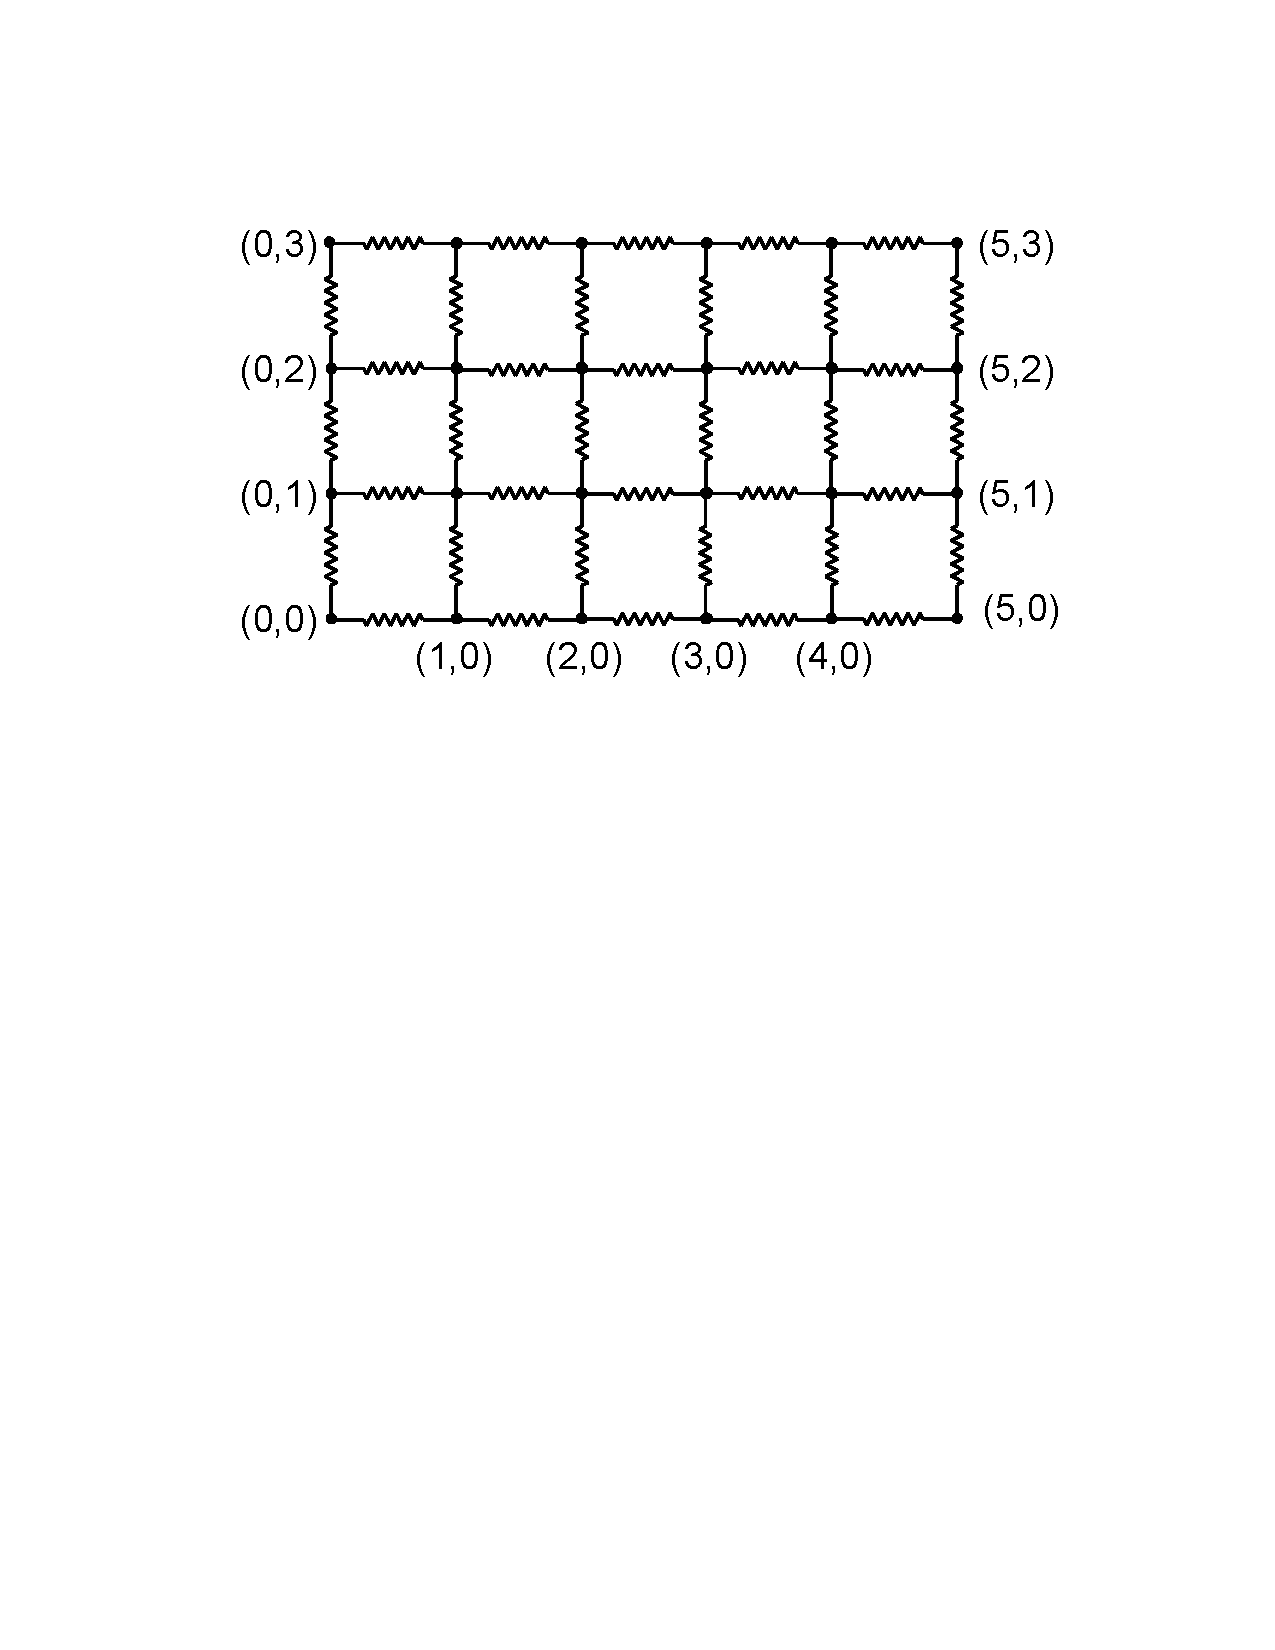
\includegraphics[width=0.60\textwidth]{Wu04fig4}
  \caption{\label{Wu04fig4}
A $[5\!\times\!4]$ rectangular resistor network:
resistors with resistances $r$ and $s$ on edges of the network in,
respectively, horizontal and vertical directions.
  }
\end{figure}
%%%%%%%%%%%%%%%%%%%%%%%%%%%%%%%%%%%%%%%%%%%%

The paper is very clear and explicit, with many examples, including the
1\dmn\ periodic chain (sect.~{\em 3.2. Periodic boundary conditions}) and
the doubly periodic $[L\!\times\!T]$ square lattice, his sect.~{\em 5.
Two-dimensional network} and \reffig{Wu04fig4}. His eq.~(43) gives the
resistance between  nodes $z_1=(x_1, y_1)$
and  $z_2=(x_2, y_2)$
 \bea
R^{[L\!\times\!T]}_{z_1 z_2}
%R_{\{M\times N\}}^{\rm per} ({\bf r}_1,{\bf r}_2)
&=&  {\sum_{m=0}^{M-1}\sum_{n=0}^{N-1}} _{(m,n) \not= (0,0)}
\frac{\Big|\psi_{(m,n);(x_1,y_1)} - \psi_{(m,n);(x_2, y_2)}\Big|^2 }{\lambda_{(m,n)}} \nonumber \\
%&=& \frac{1}{N} R_{\{M\times 1\}}^{\rm per}(x_1,x_2)
%+  \frac{1}{M} R^{\rm per}_{\{N\times 1\}}(y_1,y_2)\nonumber \\
&=& \frac{r}{N} \Bigg[\,\Big| x_1 -x_2 \Big| -\frac{(x_1-x_2)^2}{M}
\Bigg] + \frac{s}{M}\Bigg[\,\Big| y_1 -y_2 \Big| -\frac{(y_1-y_2)^2}{N}
\Bigg] \nonumber \\
&+& \frac{1}{MN} \sum_{m=1}^M \sum_{n=1}^N
\frac{1- \cos \Big[2(x_1-x_2)\theta_m+2(y_1-y_2)\phi_n \Big]}
 {r^{-1}\big(1-\cos 2\theta_m \big)+s^{-1}\big(1-\cos 2\phi_n \big)} ,\nonumber \\
&& \hskip 2cm
\label{Wu04:RR}
\eea
% where  the two terms in the second line are given by (\ref{R1Dper}).
The result depends only on the differences
$\big|x_1-x_2\big|$ and $\big|y_1-y_2\big|$, as it should
by translational invariance.
This is a double sum over Fourier modes, and I see no determinant
calculation where these are summed over and what remains is some sensible
polynomial.

However, his sect.~{\em 10.
Summation and product identities} might be just what we need:

He shows that
\bea
 F_N(\ell) &=& \frac{1}{N} \sum_{n=1}^{N-1} \frac{1-\cos (\ell \phi_n)}{1-\cos \phi_n}
\continue
            &=& |\ell| - \frac{1}{N} \Bigg(\frac{\ell^2 +|\ell|}{2}
                       - \Bigg[\frac{|\ell|}{2}\Bigg] \Bigg)
\label{Wu04:F1}
\eea
where $[x]$ denotes the integral part of $x$.
Similarly
\[
G_N(\ell)=
 \frac{1}{N} \sum_{n=1}^{N-1} \frac{1-\cos (2\ell \phi_n)}{1-\cos 2\phi_n}
\,.
\]
\medskip
is evaluated as a special case of the identity
(\ref{Wu04:I2}), using
the recursion relation
\[
G_N(\ell)-G_N(\ell-1) = 1- \frac{1}{N} \big({2\ell -1}\big) \nonumber
\]
which yields
\beq
G_N(\ell) = \big|\ell\big| - \ell^2/N
\,.
\ee{Wu04:GN}




\medskip
\noindent
{\it Proposition: Define
\[
I_\alpha (\ell) =  \frac{1}{N} \sum_{n=0}^{N-1} \frac{\cos\big(\alpha\,\ell\, \frac{n\pi}{N} \big)}
  {\cosh \lambda -\cos \big(\alpha \,\frac{n\pi}{N} \big)}, \hskip1cm \alpha=1,2
\,.
\]
Then the following identities hold for $\lambda \geq 0$, $N=1,2,\cdots,$ }
 \bea
 I_1(\ell)  &=&\frac{\cosh(N-\ell)\lambda}{(\sinh \lambda) \sinh (N\lambda)}  + \frac{1}{N} \Bigg[ \frac{1}{\sinh^2\lambda}
  + \frac{1-(-1)^\ell}{4\cosh^2(\lambda/2)}\Bigg],\ 0 \leq \ell< 2N,\nonumber \\
  \label{Wu04:I1} \\
 I_2(\ell) &=&\frac{\cosh \big(\frac{N}{2} - \ell\big) \lambda}{(\sinh \lambda) \sinh (N\lambda/2)}\, ,
          \hskip 3.2cm 0 \leq \ell< N
\,.
 \label{Wu04:I2}
 \eea
\noindent
Remarks:

\medskip
3. In the  $N\to\infty$ limit both  (\ref{Wu04:I1}) and  (\ref{Wu04:I2}) become the  integral
\[
\frac{1}{\pi} \int_0^\pi \frac{\cos (\ell \theta)}{\cosh \lambda - \cos \theta}  d\,\theta
= \frac{e^{-\ell \lambda}}{\sinh \lambda}  \quad \quad \ell \geq 0 .
\]

\medskip
4.  Set $\ell = 0$ in (\ref{Wu04:I1}), multiply by $\sinh \lambda$ and integrate over $\lambda$, we obtain the product
identity
\beq
\prod_{n=0}^{N-1} \bigg( \cosh \lambda -\cos \frac{n\pi}{N}\bigg)
= (\sinh N \lambda) \tanh ( {\lambda}/ 2).
\ee{Wu04:prod}

\medskip
5. Set $\ell = 0$ in (\ref{Wu04:I2}), multiply by $\sinh \lambda$ and integrate over $\lambda$.  We obtain the product
identity
\beq
\prod_{n=0}^{N-1} \bigg( \cosh \lambda -\cos \frac{2n\pi}{N}\bigg) = \sinh^2 ( {N\lambda}/ 2).
\ee{Wu04:prod1}


\medskip
\noindent
 Proof:

\medskip
Introduce
\bea
S_\alpha(\ell) =
\frac{1}{N} \sum_{n=0}^{N-1} \frac{\cos(\ell\, \theta_n)}
  {1+a^2 -2a\cos \theta_n}, \hskip 1cm a<1 , \quad \alpha=1,2 \label{Wu04:SL}
\eea
so that
\beq
I_\alpha(\ell) = 2\, a\, S_\alpha(\ell), \hskip1cm  a=e^{-\lambda}.
\eeq
 It is readily seen that we have the identity
\beq
S_\alpha(1) = \frac{1}{2a} \Big[ (1+a^2) S_\alpha (0)-1\Big]. \label{Wu04:S10}
\eeq

\medskip
\noindent
1. Proof  of (\ref{Wu04:I1}):

\medskip
First we evaluate $S_1(0)$ by carrying
 out the following summation, where ${\cal R}$e denotes the real part,
in two different ways.  First we have
\bea
{\cal {R}}e\,
\frac{1}{N} \sum_{n=0}^{N-1}
  \frac{1}{ 1- a\, e^{i\theta_n}}
 &=& {\cal {R}}e\, \frac{1}{N} \sum_{n=0}^{N-1}
  \frac{1-a \, e^{-i\theta_n}}{\Big| 1- a\, e^{i\theta_n}\Big|^2} \nonumber \\
&=& \frac{1}{N} \sum_{n=0}^{N-1} \frac{1-a \cos \theta_n}{1+a^2-2a\cos \theta_n} \nonumber \\
&=& S_1(0) -a S_1(1) \nonumber \\
&=& \frac{1}{2} \Big[1+ (1-a^2)  S_1(0)\Big].  \label{Wu04:I11}
\eea
Secondly by expanding the summand we have
\bea
{\cal {R}}e\,\frac{1}{N} \sum_{n=0}^{N-1}
  \frac{1}{ 1- a\, e^{i\theta_n}}
={\cal {R}}e\,\frac{1}{N} \sum_{n=0}^{N-1} \sum_{\ell=0}^\infty a^\ell e^{i\ell n\pi/N}
 \nonumber
\eea
and carry out the summation over $n$
for fixed $\ell$.
  It is clear that all $\ell=$ even terms vanish except those with $\ell = 2 m N, m=0,1,2,...$
which yield $\sum_{m=0}^\infty a^{2mN} =1/(1-a^{2N})$.
For $\ell = $ odd $=2m+1,$ $m=0,1,2,...$ we have
\bea
{\cal {R}}e\, \sum_{n=0}^{N-1} e^{i(2m+1) n\pi/N}
   = {\cal {R}}e\,\frac{1-(-1)^{2m+1}}{1-e^{i(2m+1)\pi/N}} = 1 \nonumber
\eea
after making use of % (\ref{Wu04:12}),
\beq
{\cal R}e\,\Bigg( \frac{1}{1-e^{i\theta}} \Bigg)= \frac{1}{2}, \hskip1cm
 0<\theta <2\pi
 \,.
\ee{Wu04:12}
So the summation over $\ell=$ odd terms  yields
$N^{-1}\sum_{m=0}^\infty a^{2m+1} =a/N(1-a^{2})$, and  we have
\beq
{\cal {R}}e\, \sum_{n=0}^{N-1}\frac{1}{ 1- a\, e^{i\theta_n}}
   =  \frac{1}{1-a^{2N}} +\frac{a}{N(1-a^2)} \label{Wu04:I12}
\eeq
Equating (\ref{Wu04:I11}) with  (\ref{Wu04:I12})  we obtain
\beq
S_1(0) = \frac{1}{1-a^2} \Bigg[ \Bigg(\frac{1+a^{2N}}{1-a^{2N}}\Bigg)
  + \frac{2a}{N(1-a^2)} \Bigg]
  \,.
\label{Wu04:SN1}
\eeq

\medskip
To evaluate $S_1(\ell)$ for general $\ell$,  we
consider the summation
 \bea
{\cal {R}}e\,
\frac{1}{N}\sum_{n=0}^{N-1}
  \frac{1-\big(a\, e^{i \theta_n}\big)^\ell} { 1- a\, e^{i \theta_n}}
 &=& {\cal {R}}e\,
\frac{1}{N}\sum_{n=0}^{N-1}
  \frac{(1-a^\ell\, e^{i \ell \theta_n})(1-a\, e^{-i\theta_n})}
       {\big|1- a\, e^{i \theta_n}\big|^2}
\label{Wu04:I41}\\
&=&  S_1(0) - a S_1(1) - a^\ell S_1(\ell) +a^{\ell+1} S_1(\ell-1)
\,,
\nonumber
\eea
where the second line is obtained by writing out  the real part of the summand as in (\ref{Wu04:I11}).
 On the other hand, by expanding the summand we have
\bea
{\cal {R}}e\,
\frac{1}{N} \sum_{n=0}^{N-1}
  \frac{1-\big(a\, e^{i \theta_n}\big)^\ell} { 1- a\, e^{i \theta_n}} &=&
{\cal {R}}e\,
\frac{1}{N} \sum_{n=0}^{N-1} \sum_{m=0}^{\ell -1} a^m e^{i\pi m  n/N} \nonumber \\
&=& 1+{\cal {R}}e\,
\frac{1}{N} \sum_{m=1}^{\ell-1} a^m \Bigg(\frac{1-(-1)^m}{1-e^{i\pi m/N}} \Bigg) \nonumber \\
&=& 1+\frac{a(1-a^\ell)} {N(1-a^2)}, \quad \ell = {\rm even}< 2N \nonumber \\
&=& 1+\frac{a(1-a^{\ell-1})} {N(1-a^2)}, \quad \ell = {\rm odd} <2N
\,,
\label{Wu04:I42}
\eea
where again we have used (\ref{Wu04:12}).

\medskip
 Equating (\ref{Wu04:I42}) with (\ref{Wu04:I41}) and using
(\ref{Wu04:S10})   and (\ref{Wu04:SN1}),
 we obtain the recursion relation
\beq
S_N(\ell)-a\,S_N(\ell-1)=A\,a^{-\ell} +B_\ell
\ee{Wu04:Q}
 where
\bea
A =\frac{a^{2N}}{1- {a^{2N}} }, \hskip 1cm B_\ell = \frac{a^{(1+(-1)^\ell)/2} }{ N(1-a^2)} .
\eea

The recursion relation (\ref{Wu04:Q}) can be solved by standard means.  Define
 the generating function
\beq
G_\alpha(t) =\sum_{\ell =0}^\infty S_\alpha(\ell)\, t^\ell, \hskip1cm \alpha=1,2
\,.
\ee{Wu04:gen}
Multiply (\ref{Wu04:Q}) by $t^\ell$ and sum over $\ell$.  We obtain
\bea
(1-at)G_1(t) -S_1(0) = \frac{A\,a^{-1}t}{1-a^{-1}t} + \frac{t+at^2} {N(1-a^2)(1-t^2)}.
\eea
This leads to
\bea
G_1(t) &=& \frac{1}{1-at} \Bigg[ S_1(0) +\frac{A\,a^{-1}t}{1-a^{-1}t} +
\frac{t+at^2} {N(1-a^2)(1-t^2)} \Bigg] \nonumber \\
 &=&\frac{1}{(1-a^2)(1-a^{2N})} \Bigg[\frac{1}{1-at}
  +\frac{a^{2N} }{1-a^{-1}t} \Bigg] \nonumber \\
&&+\, \frac{1}{2N(1-a)^2(1-t)} -\frac{1}{2N(1+a)^2(1+t)},\nonumber
\eea
from which one obtains
\bea
S_1(\ell) &=& \frac{a^\ell +a^{2N-\ell}} {(1-a^2)(1-a^{2N})}
+ \frac{1}{2N(1-a)^2} - \frac{(-1)^\ell}{2N(1+a)^2} \nonumber \\
&=& \frac{a^\ell +a^{2N-\ell}} {(1-a^2)(1-a^{2N})}
+\frac{1}{2N} \Bigg[\frac{4a} {(1-a^2)^2} +\frac{1-(-1)^\ell}{(1+a^2)^2}\Bigg].
\eea
It follows that using
 $I_1(\ell) = 2\,a\, S_1(\ell)$
we obtain (\ref{Wu04:I1}) after setting $a=e^{-\lambda}$.

\medskip
\noindent
2. Proof of (\ref{Wu04:I2}):

\medskip
Again, we first evaluate $S_2(0)$ by carrying out the summation
\[
{\cal {R}}e\,
\frac{1}{N} \sum_{n=0}^{N-1}
  \frac{1}{ 1- a\, e^{i2\theta_n}}, \hskip1cm a<1
\]
in two different ways.  First as in
(\ref{Wu04:I11}) we have
\bea
{\cal {R}}e\,
\frac{1}{N} \sum_{n=0}^{N-1}
  \frac{1}{ 1- a\, e^{i2\theta_n}}
  = \frac{1}{2} \Big[1+ (1-a^2)  S_2(0)\Big], \label{Wu04:I21}
\eea
where $S_2(\ell)$ is defined in (\ref{Wu04:SL}).
 Secondly by expanding the summand we have
\beq
\frac{1}{N} \sum_{n=0}^{N-1}
  \frac{1}{ 1- a\, e^{i2\theta_n}}
=\frac{1}{N} \sum_{n=0}^{N-1} \sum_{\ell=0}^\infty a^\ell e^{i2\ell n\pi/N}
=\frac{1}{1-a^N}
\ee{Wu04:I22}
where by carrying out the summation over $n$
for fixed $\ell$ all terms in (\ref{Wu04:I12})
vanish except those with $\ell = m N, m=0,1,2,...$
 Equating
(\ref{Wu04:I22}) with (\ref{Wu04:I21})  we obtain
\bea
  S_2(0)= \frac{1}{1-a^2} \Bigg(\frac{1+a^N}{1-a^N} \Bigg) \label{Wu04:SN2}
\eea
and from (\ref{Wu04:S10})
\bea
S_2(1) = \frac{1}{1-a^N}. \nonumber
\eea
We consider next the summation
\beq
 {\cal {R}}e\,
\frac{1}{N} \sum_{n=0}^{N-1}
  \frac{1-\big(a\, e^{i2 \theta_n}\big)^\ell}{ 1- a\, e^{i2 \theta_n}} \hskip1cm a<1
  \,.
\ee{Wu04:I20}
Evaluating the real part of the summand directly as in (\ref{Wu04:I41}), we obtain
\bea
{\cal {R}}e\,
\frac{1}{N} \sum_{n=0}^{N-1}
  \frac{1-\big(a\, e^{i2 \theta_n}\big)^\ell}{1- a\, e^{i2 \theta_n}} =
  S_2(0) - a S_2(1) - a^\ell S_2(\ell) +a^{\ell+1} S_2(\ell-1).\label{Wu04:I23}
 \eea
   Secondly, expanding the summand in (\ref{Wu04:I20}) we obtain
\bea
\frac{1}{N} \sum_{n=0}^{N-1}
  \frac{1-\big(a\, e^{i2 \theta_n}\big)^\ell} { 1- a\, e^{i2 \theta_n}}
 &=& \frac{1}{N} \sum_{n=0}^{N-1}
  \sum_{m=0}^{\ell-1} a^m e^{i2\pi mn/N} \nonumber \\
&=& \frac{1}{N} \Bigg[ N + \sum_{m=1}^{\ell-1} \frac{1-e^{i2m\pi}}{1-e^{i2m\pi/N}}\Bigg] \nonumber \\
&=& 1 \hskip 2cm m<\ell \leq N . \label{Wu04:I24}
\eea
 Equating (\ref{Wu04:I24}) and (\ref{Wu04:I23}) and making use of (\ref{Wu04:SN2})
for $S_2(0)$, we obtain
\bea
S_2(\ell) -a S_2(\ell-1) = \frac{a^{N-\ell}}{1-a^N}  \label{Wu04:rec1}
\eea

The recursion relation (\ref{Wu04:rec1}) can be solved as in the above.
Define the generating function $G_2(t)$ by (\ref{Wu04:gen}).
 We find
\bea
G_2(t) &=&
\frac{1}{1-at}\Bigg[S_2(0) + \frac{a^{N-1}t}{(1-a^N) (1-a^{-1}t)} \Bigg] \nonumber \\
 &=& \frac{1}{(1-a^2)(1-a^{2N})} \Bigg[\frac{1}{ 1-at} + \frac{a^N}{ 1-a^{-1}t}\Bigg],
\eea
from which one reads off
\[
S_2(\ell) = \frac{a^\ell +a^{N-\ell}} {(1-a^2)(1-a^{2N})}.
\]
Using the relation $I_2(\ell) = 2\, a\, S_2(\ell)$ with $ a=e^{-\lambda}$, we obtain (\ref{Wu04:I2}).


\item[2019-11-04 Predrag]
Tzeng and Wu have extended this impedance networks, where the
Laplacian matrix has complex matrix elements; I think we do not care
about this at this time.


\item[2019-11-04 Predrag]
The corner-to-corner resistance and its asymptotic expansion for various
boundary conditions were calculated by Izmailian and Huang\rf{IzmHua10}
{\em Asymptotic expansion for the resistance between two maximally
separated nodes on an {$M$} by {$N$} resistor network}:
``
The computation of the asymptotic expansion of the corner to-corner
resistance, in other word the resistance between two maximally separated
nodes of a rectangular resistor network is of interest as its value
provides a lower bound to the resistance of compact percolation clusters
in the Domany-Kinzel model of a directed percolation [15]. ''

They take a $[\speriod{}\times\period{}]$ array, use a ton of funky
identities, and manage to reduce Wu's double sum \refeq{Wu04:RR} to a
single, highly non-obvious sum, their eq.~(33).
Then there are Kronecker's double series
expressed in terms of the complete elliptic integrals $K(s)$ and $E(s)$.

\item[2020-01-11 Predrag] Dienstfrey, Hang and Huang\rf{DiHaHu01} {\em
Lattice sums and the two-dimensional, periodic {Green's} function for the
{Helmholtz} equation}.
They compute the Green's function for the Helmholtz equation in two
dimensions with doubly periodic boundary conditions, on a fundamental
cell $[-1/2,12)^2$. I believe this is not relevant to us, it solves a
continuous problem over the unit cell, rather than a problem on discrete
lattice.

Due to the translation invariance, the Green's function has a convolution
structure,
\(
G(x,x_0)= G(y)
\,,\quad y=x-x_0
\in[-1,1)^2
\,.
\)
A periodic Helmholtz equation can be computed via the method of images
over the zeroth-order Hankel function of the first-kind. The sums can
also be evaluated by recognizing an identity between the so-called
`spectral' and `spatial' representations of $G$. For a square array,
there are symmetries which allow for further simplification.

\item[2020-01-10 Predrag]
Stewart and G{\"o}kaydin\rf{SteGok19}
{\em Symmetries of quotient networks for doubly periodic patterns on the
square lattice}, \CBlibrary{SteGok19}. Read for
\refsect{sect:fundDomHL}~{\em Reduction to the fundamental domain} that has still
to be completed.

\item[2020-01-10 Predrag]
A very pedagogical, down to earth textbook:
Pozrikidis\rf{Pozrikidis14}
{\em An introduction to grids, graphs, and networks},
\CBlibrary{Pozrikidis14}:

\emph{Graphs} are finite or infinite sets of vertices connected by edges in
structured or unstructured configurations.

Infinite \emph{lattices} and tiled surfaces are described by highly ordered graphs
parametrized by an appropriate number of indices.

\emph{Networks} consist of nodes connected by physical or abstract links
with an assigned conductance in spontaneous or engineered configurations.
In physical and engineering applications, networks are venues for
conducting or convecting a transported entity, such as heat, mass, or
digitized information according to a prevailing transport law.

\emph{Finite difference} and finite element \emph{grids} can be regarded
as networks whose link conductance is determined by the differential
equation, as well as by the chosen finite difference or finite element
approximation.

A finite difference grid for solving ordinary or partial differential
equations consists of rectilinear grid lines that can be regarded as conveying
links intersecting at nodes.

Topics:
The node adjacency, Laplacian, and Kirchhoff matrices;
The computation of the regular and generalized lattice Green's function
describing the response to a nodal source;
The pairwise resistance of any two nodes.

Consider the Poisson equation in one dimension for an unknown function of one
variable, $f(x)$,
\beq
\frac{d^2 f}{dx^2} + g(x) = 0
\,,
\ee{Pozrikidis14(1.1.1)}
to be solved in a finite domain, [a, b], where $g(x)$ is a given source
function. When $g(x) = 0$, the Poisson equation reduces to Laplace's
equation. When $g(x) = {\alpha}f(x)$, the Poisson equation reduces to
the Helmholtz's equation,
\beq
\left(\frac{d^2 ~}{dx^2} + {\alpha}\right)f(x) = 0
\,,
\ee{Pozrikidis14(1.1.11)}
where $\alpha$ is a real or complex constant.
(See also \refsect{sect:Helmoltz}~{\em Helmoltz and screened Poisson
equations}.)



Applying the Poisson equation at the $i$th node, approximating the second
derivative with a central difference
\beq
f_{i+1} - 2f_{i} + f_{i-1} = - g_{i}
\ee{Pozrikidis14(1.1.3)}
where $f_{i} = f (x_{i})$, $g_{i} = g(x_{i})$.
He says: ``The signs on the left- and right-hand sides of
\refeq{Pozrikidis14(1.1.3)} were chosen intentionally to conform with
standard notation in graph theory regarding the Laplacian, as discussed
in Section 1.7.''

The discretized Helmholtz's equation:
\beq
f_{i+1} - 2f_{i} + f_{i-1} + {\alpha}f_{i} = 0
\,,
\ee{Pozrikidis14(1.1.11H)}
so for us ${\alpha}=2-s$.

For any boundary conditions -Neumann, Dirichlet, or
periodic- the coefficient matrix of the linear system admits the factorization
\beq
L = R\transp{R}
\ee{Pozrikidis14(1.1.6)}
where $R$ is a square or rectangular matrix.
This factorization is the discrete counterpart of the second
derivative constructed as the sequential application of the first derivative.
Note that the commutative property $R\transp{R}=\transp{R}R$ is not always
satisfied.

When the Dirichlet boundary condition is specified at both ends of the
solution domain, the first and last values, $f_{1}$ and $f_{n+1}$, are
known. Collecting the difference equations \refeq{Pozrikidis14(1.1.3)}
for the interior nodes, $i = 2,. . . , n$, we obtain a system of linear
equations where $L$ is $(n-1)\times(n-1)$ symmetric tridiagonal Toeplitz
matrix, a matrix with constant diagonal lines. The $m=1,2,\cdots,n-1$
eigenvalues of $L$ are
\beq
\lambda_m = 2-2\cos\alpha_m = 4 \sin^2\left(\half\alpha_m\right)
\,,\quad
\alpha_m=\pi\frac{m}{n}
\ee{Pozrikidis14(1.2.7)}
% (Predrag: for some reason, in our papers we never state the
% $\sin^2\left(\half\alpha_m\right)$ version of the eigenvalues.)

He also lists eigenvectors and factorizes as in
\refeq{Pozrikidis14(1.1.6)}, and discusses the Neumann boundary condition,
in which case $L$ is a ``nearly Toeplitz matrix.''
as well. In factorization \refeq{Pozrikidis14(1.1.6)}, $R$ is now a rectangular matrix.

For periodic boundary conditions, $L$ is a ``nearly tridiagonal matrix.''
Because of the zero eigenvalue of the Laplacian, $\lambda_0= 0$,
corresponding to a constant eigenvector, the matrix $L$ is singular. The
rest of the eigenvectors are pure harmonic waves. The identity
\beq
\transp{f}\cdot{L}\cdot{f} = \sum_{i=1}^n (f_{i+1} - f_{i})^2 \geq 0
\ee{Pozrikidis14(1.6.11)}
for arbitrary periodic field $f$ demonstrates that the matrix $L$ is
positive semidefinite.

The periodic Laplacian is a circulant matrix.

He defines the graph Laplacian.

The adjacency matrix $A$, defined as $A_{ij}=1$ if nodes $i$ and $j$ are
connected by a grid line or link, 0 otherwise, with the convention that
$A_{ii}=0$. Thus, by convention, the diagonal line of the adjacency
matrix is zero. .

The number of paths that return to an arbitrary node after $s$ steps have
been made, summed over all starting nodes, is
\beq
n_s = \sum_{j=1}^n \mu^2_j
\ee{Pozrikidis14(1.7.7)}
where $\mu_j$ are eigenvalues of $A$.

The degree of the $i$th node, denoted by $d_i$, is defined as the number
of links attached to the node, which is equal to the sum of the elements
in the corresponding row or column of the adjacency matrix. The Laplacian
equals $L=D-A$, where $D$ is a diagonal matrix whose $i$th diagonal
element is equal to the corresponding node degree $d_i$.

He introduces the oriented incidence matrix $R$, by labeling nodes and
links sequentially, and shows it leads to the  factorization
\refeq{Pozrikidis14(1.1.6)}. All of these notions generalize to graphs.

A uniform two-dimensional Cartesian (square) lattice.

An Archimedean lattice consists of an infinite doubly periodic array
regular polygons. In particular, each node is surrounded by the same
sequence of polygons. There are 11 Archimedean lattices.

The Archimedean $4^4$ lattice, also known as the square lattice, is a
Bravais lattice consisting of a doubly periodic array of empty squares.

Laves lattices are the duals of the Archimedean lattices. A Laves lattice
arises by introducing vertices in the middle of the tiles (faces) of an
Archimedean lattice and then connecting the vertices to cross the edges
of the Archimedean lattice. The dual of the square lattice is the same
square lattice.

The nodes of a two- or three-dimensional regular lattice, regarded as a
structured network, can be identified by two or three indices assigned to
the individual lattice directions. The  spectra of lattice networks
Laplacians are used in computing of lattice Green's functions.

His \reffig{fig:Pozrikidis14_2-2-1} is interesting: I think it is a plot of
the lowest eigenstates (``spectral partitioning'') of a $[17\times17]$
square lattice (``Cartesian network'') consisting of a complete set
of horizontal and vertical links.
As an example, the spectral partitioning of a square network is shown in
Figure 2.2.1.
%%%%%%%%%%%%%%%%%%%%%%%%%%%%%%%%%%%%%%%%%%%%
\begin{figure}
  \centering
  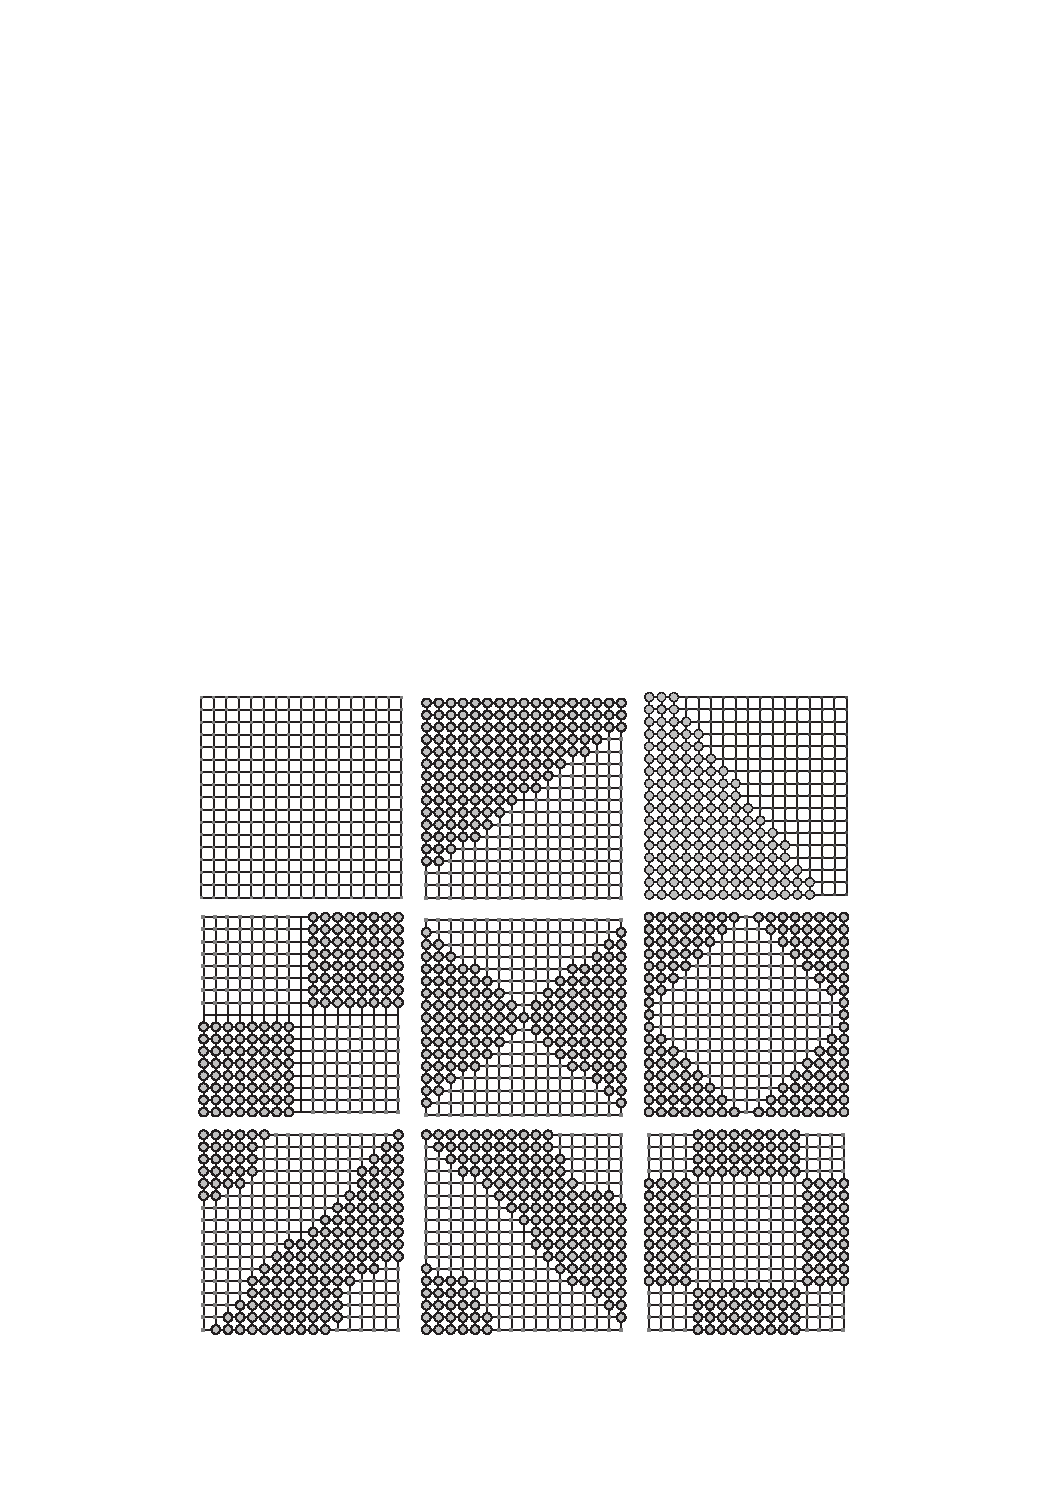
\includegraphics[width=0.70\textwidth]{Pozrikidis14_2-2-1}
  \caption{\label{fig:Pozrikidis14_2-2-1}
A $[17\times17]$ rectangular Helmholtz \refeq{Pozrikidis14(1.1.11H)}
network. Positive components of an eigenvector are marked as filled
circles, negative components are marked as dots, and zero components are
unmarked. The network shown consists of $N=17^2=289$ nodes connected by
$L=544$ links. The degree of the 4 corner nodes is 2, the 60 edge nodes
is 3, and 225 interior nodes is 4. Exact expressions for the eigenvalues
and eigenvectors of the Laplacian of the square network are discussed in
Pozrikidis Chapter 3. The first nine eigenvalues corresponding to the
eigenvectors shown here are $\lambda_i=0$, 0.0341 (double), 0.0681,
0.1351 (double), 0.1691 (double), and 0.2701.
Pozrikidis\rf{Pozrikidis14} Fig~2.2.1.
  }
\end{figure}
%%%%%%%%%%%%%%%%%%%%%%%%%%%%%%%%%%%%%%%%%%%%

In
spectral partitioning (a weighed
sum of eigenvectors of the Laplacian matrix)
%relies on the zero-mean property expressed by ,
roughly an equal number of eigenvector components with positive
and negative sign appear.
Eigenvector corresponding to the zero eigenvalue of the Laplacian matrix
is uniform over the nodes of a network; the eigenvector corresponding to
the zero eigenvalue is filled with ones. Orthogonality of the set of
eigenvectors requires that all other eigenvectors have mean zero, his
Eq.~(2.2.8). Higher eigenvectors partition the network into two or a
higher number of pieces (spectral partitioning). To partition a network,
we may group together nodes whose eigenvector components corresponding to
a specified eigenvalue have the same sign. The eigenvalue with the second
smallest magnitude, is chosen for division into two fragments, while
higher eigenvalues are chosen for division into a higher number of
fragments.

A network whose structure is isomorphic to that of a square lattice
consists of two intersecting one-dimensional arrays of links. A theorem
due to Fiedler\rf{Fiedler73,AndMor85} states that the eigenvectors of the
Laplacian matrix for certain types of boundary conditions are tensor
products of those of the constituent one-dimensional graphs, and the
eigenvalues are the sums of the eigenvalues of the Laplacian of the
constituent one-dimensional graphs. This property reflects the
separability of the discrete Laplace operator in Cartesian coordinates.

We need to understand \catlatt\ eigenmodes. If $s<2$ lattice is a spring
mattress, with spring constant $2-s$, what are the normal modes of the
$s>2$ \catlatt?
In the above he discusses the Helmholtz, $s=2$ Laplacian eigenmodes
case \refeq{Pozrikidis14(1.1.11H)}.

\item[2020-01-21 Predrag]
Fruchart, Zhou and Vitelli\rf{FrZhVi20}
{\em Dualities and non-{Abelian} mechanics} seems interesting.
The abstract:
``
Dualities are mathematical mappings that reveal links between apparently
unrelated systems in virtually every branch of physics.
Systems mapped onto themselves by a duality transformation are called
self-dual and exhibit remarkable properties, as exemplified by the scale
invariance of an Ising magnet at the critical point. Here we show how
dualities can enhance the symmetries of a dynamical matrix (or
Hamiltonian), enabling the design of metamaterials with emergent
properties that escape a standard group theory analysis. As an
illustration, we consider twisted kagome lattices,
reconfigurable mechanical structures that change shape by means of a
collapse mechanism. We observe that pairs of distinct configurations
along the mechanism exhibit the same vibrational spectrum and related
elastic moduli. We show that these puzzling properties arise from a
duality between pairs of configurations on either side of a mechanical
critical point. The critical point corresponds to a self-dual structure
with isotropic elasticity even in the absence of spatial symmetries and a
twofold-degenerate spectrum over the entire Brillouin zone. The spectral
degeneracy originates from a version of Kramers' theorem in which
fermionic time-reversal invariance is replaced by a hidden symmetry
emerging at the self-dual point. The normal modes of the self-dual
systems exhibit non-Abelian geometric phases that affect the
semiclassical propagation of wavepackets, leading to non-commuting
mechanical responses.
''

Mechanical structures are described at the linear level by normal modes
of vibration and their oscillation frequencies. Both are determined by
the dynamical matrix $\hat{D}$, which summarizes the Newton equations of motion
in the harmonic approximation [...] our analysis also applies
when $\hat{D}$ is replaced by other linear operators, such as the Maxwell
operator of a photonic crystal[ref28], the mean-field Hamiltonian of a quantum
system (in which case the eigenvalues are energies) or the dynamical
matrix of an electrical circuit\rf{NOSSS15,AlGlJi15,LIBBBMKT18}.

A \emph{symmetry} is a transformation that maps a system onto itself.
A \emph{duality} relates distinct models or structures.
In self-dual systems, the distinction between dualities and symmetries is
blurred: additional symmetries can emerge at a self-dual point even if
the spatial symmetries are unchanged.
Such dualities can be harnessed to engineer material properties from wave
propagation to static responses that are not predicted by a standard
symmetry analysis based on space groups.
    \index{symmetry}\index{duality}



This one as well:
Souslov and Vitelli\rf{SouVit19} {\em Geometry for mechanics}:
``
The mechanics of many materials can be modelled by a network of balls
connected by springs. A bottom-up approach based on differential geometry
now captures changes in mechanics upon network growth or merger, going
beyond the linear deformation regime.
''

\item[2021-01-09 Predrag]
Fruchart, Zhou and Vitelli\rf{FrZhVi20} cite

Ningyuan \etal\rf{NOSSS15}
{\em Time- and site-resolved dynamics in a topological circuit}:
I think we can ignore this paper. Though supplemental material explains:
(1) The Harper-Hofstadter model, and its extension to spinful systems.
(2) Photonic lattices, in both massive and massless limits.
(3) Adding topology to photonic lattice models.
(4) Mathematical tools for the calculation of band-structure,
corresponding band Chern numbers, and two-point response of photonic
lattice models.
(5) Mathematical tools for calculating band- and edge- structure of
finite strips.

Albert, Glazman and Jiang\rf{AlGlJi15}
{\em Topological properties of linear circuit lattices}
have a 3-site lattice example, where the Lagrangian contribution of the
link between neighboring sites is built from
a (kinetic) capacitive part with what we call {\jacobianOrb} \jMorb,
and a (potential)
inductive part with what we call shift matrix $\shift$.

\item[2021-01-09 Predrag]
Fruchart, Zhou and Vitelli\rf{FrZhVi20} cite
Lee \etal\rf{LIBBBMKT18} {\em Topolectrical circuits}.
The normal mode frequency matrix of our circuit is unitarily equivalent
to the hopping matrix of a quantum spin Hall insulator.

Circuits consisting of resistor, inductor and capacitor (RLC) components
are governed by its circuit Laplacian, which is analogous to the
Hamiltonian describing the energetics of a physical system. Here we show
that topological insulating and semimetallic states can be realized in a
periodic RLC circuit.

Any electrical circuit network can be represented by a graph whose nodes
and edges correspond to the circuit junctions and connecting
wires/elements. The circuit behavior is fundamentally described by
Kirchhoff's law. As an initial step towards identifying circuits with
tight-binding lattice models, they rewrite Kirchhoff's law in a matrix
form, and consider circuits made up of periodic sublattices, with
periodic boundary conditions (i.e. without grounded terminations).

What we call {\jacobianOrb} \jMorb\ they call `the grounded Laplacian'
$\jMorb$.

The regularized inverse of $\jMorb$ known as the circuit Green's function
(regularization in this context means that 0 modes are omitted).
The Laplacian is defined in terms of the conductances by $L=D-C$,
where $C$ is the (adjacency) matrix of conductances and
$D$ lists the total conductances out of each node.
They call the set of eigenvalues the bandstructure of the circuit, and
also refer to the nodes as sites.

RLC circuits obey a linear 2nd order ordinary differential equation
(ODE), just like a mechanical system with springs, dampers and masses.






\end{description}

\renewcommand\speriod[1]{{\ensuremath{L_{#1}}}}  %continuous spatial period
\renewcommand\period[1]{{\ensuremath{T_{#1}}}}  %continuous time period


\newpage %TEMP
% siminos/spatiotemp/catMapLatt.tex
% $Author: predrag $ $Date: 2020-12-14 00:22:48 -0500 (Mon, 14 Dec 2020) $

\section{Counting {\twots}}
\label{s:2DcatCounting}
% until 2019-08-13 was siminos/kittens/twots2D.tex      pdflatex CL18

%%%%%%%%%%%%%%%%%%%%%%%%%%%%%%%%%%%%%%%%%%%%%%%%%%%%%%%%%%%%%%%%%%%%%%%%
	\HL{2019-06-25}{
    This section is a version of kittens refsect~{s:dDcatMap}
    that starts from 2D cat map
    without giving the formula of general $d$\dmn\ \catlatt. I feel
    this is less clear than start with the $d$\dmn\ \catlatt, but
    it directly follows the section of {\spt} cat map.
    Eventually this text was not used not used in kittens\rf{CL18}.
    }
An {\twot} on a 2\dmn\ {\spt}ly infinite $\integers^2$ lattice has
more complicated pattern than a cat map \po. An
{\twot} can tile the infinitely large 2\dmn\ space not only by
repeating in the time or space direction, but also by moving in both of
the {\spt} directions. The repeating pattern can generally be described
by a Bravais lattice:
\beq
\lattice = \{n_1 {\bf a}_1 + n_2 {\bf a}_2 | n_i \in \mathbb{Z}\}.
\ee{2DBravLatt}
And the {\twots} tile the infinitely large 2\dmn\ space by:
\beq
\ssp_{{\bf z}} = \ssp_{{\bf z}+{\bf R}} \, , \quad {\bf R} \in \lattice \, .
\ee{2DPeriodicField}
The ${\bf z}$ here is a two\dmn\ vector which labels the position and time of the field.
The {\sPe} \refeq{2dCoupledCats} can be written as:
\beq
(-2s + \sigma_1 + \transp{\sigma}_{1} + \sigma_2 + \transp{\sigma}_{2}) \ssp_{\bf z} = -m_{\bf z} \, ,
\ee{2DCat}
where the $\sigma_i$ is a translation operator which can translate the
field in the positive $i$th direction by length one and
$\transp{\sigma}_{i}$ is the inverse of the operator $\sigma_i$ which
translates the field in the negative $i$th direction. Here we can assume
that $\sigma_1$ is a translation in the time and $\sigma_2$ is a
translation in space. But since the system is invariant under the
exchange of space and time, we don't need to distinguish these two
directions.

Note that in \refeq{2DCat} the operators, field and source are defined on
infinitely large 2\dmn\ space (lattice). For an {\twot}, which is
a periodic tile, the {\sPe} \refeq{2DCat} is also satisfied
on this finite tile. But in this case, the translation operators need to
satisfy the periodic {\bcs} specified by this {\twot}. And
the
$-2s +\sigma_1 +\transp{\sigma}_{1} +\sigma_2 +\transp{\sigma}_{2}$
on the finite region is the {\jacobianOrb} matrix of this specific periodic
pattern.

Following the same procedure as counting the periodic points of a cat
map, we know that the number of periodic points is given by the
determinant of the {\jacobianOrb}. To find the determinant and the
inverse of the {\jacobianOrb}, we need to first find the eigenvectors
and eigenvalues.

The eigenvectors here are fields defined in this finite tile. The
elements of these eigenvectors are generally complex numbers. If we tile
the whole 2\dmn\ space with one of these finite fields using the periodic
condition, we will get an eigenvector of the operator in \refeq{2DCat}
defined in the infinite 2\dmn\ space. And the eigenvalue remains
unchanged. So we can find the eigenvectors and eigenvalues in the
infinite 2\dmn\ space then reduce the field into the finite tiles.

	\HL{2019-06-17}{
	I will need to rewrite this paragraph to make it clearer.
	}

For a 2\dmn\ {\spt} cat map, we want to find eigenvectors with
periodicity given by the Bravais lattice \refeq{2DBravLatt}, where ${\bf
a}_1$ and ${\bf a}_2$ are two 2\dmn\ basis vectors. The general form of
these basis vectors are ${\bf a}_1 = \{l_1, l_2\}$ and ${\bf a}_2 =
\{l_3, l_4\}$. For a given Bravais lattice, the choice of basis vectors
is not unique. It is shown by Lind\rf{Lind96}, \CBlibrary{Lind96} that we can choose basis
vectors with form ${\bf a}_1 = \{l_1, 0\}$ and ${\bf a}_2 = \{l_3, l_4\}$
without loss of generality.
    \PC{2020-02-15}{
    This is called `Hermite normal form', see
    \refeq{Holmin12-Hermite}.
    }
Then the reciprocal lattice is:
\beq
\overline{\lattice} = \{n_1 {\bf b}_1 + n_2 {\bf b}_2 | n_i \in \mathbb{Z}\}
\,,
\ee{2DReciprLatt}
where the vectors ${\bf b}_1$ and ${\bf b}_2$ satisfy:
\beq
{\bf b}_i \cdot {\bf a}_j = 2 \pi \delta_{ij}
\,.
\ee{2DReciprocalVectors}
The eigenvectors of the translation operator which satisfy the
periodicity of the Bravais lattice \refeq{2DBravLatt} are
plane waves of form:
\beq
f_{\bf k}({\bf z}) = e^{i {\bf k} \cdot {\bf z}}
  \,, \quad
{\bf k} \in \overline{\lattice}
\,,
\ee{2DEigenvect}
where the wave vector ${\bf k}$ is on the reciprocal lattice
$\overline{\lattice}$. For the basis vectors ${\bf a}_1 = \{l_1, 0\}$
and ${\bf a}_2 = \{l_3, l_4\}$, the basis vectors of the corresponding
reciprocal lattice are ${\bf b}_1 = 2 \pi / l_1 l_4 \, \{l_4, -l_3\}$ and
${\bf b}_2 = 2 \pi / l_1 l_4 \, \{0, l_1\}$. The expression of
eigenvector with wave vector ${\bf k} = n_1 {\bf b}_1 + n_2 {\bf b}_2$
is:
\beq
f_{\bf k}({\bf z}) = e^{i {\bf k} \cdot {\bf z}} = \exp[i\frac{2 \pi}{l_1 l_4}(n_1 l_4 z_1 - n_1 l_3 z_2 + n_2 l_1 z_2)] \, ,
\ee{2DEigenvect1}
where the ${\bf z}=(z_1,z_2)$. The eigenvalue of the operator $s -
\sigma_1 - \transp{\sigma}_{1} - \sigma_2 - \transp{\sigma}_{2}$
corresponding to this eigenvector is:
\beq
\lambda_{\bf k} = s - 2 \cos(\frac{2 \pi n_1}{l_1}) - 2 \cos(-\frac{2 \pi n_1 l_3}{l_1 l_4} + \frac{2 \pi n_2}{l_4})
\, .
\ee{2DEigenval}
It is sufficient to use the wave vectors ${\bf k}$ with $n_1$ from 0 to
$l_1-1$ and $n_2$ from 0 to $l_4-1$ to get all of the eigenvectors. Any
wave vector on the reciprocal lattice outside of this range will give an
eigenvector which is equivalent to an eigenvector with the wave vector in
the range. So the number of eigenmodes we can get is $l_1 l_4$, which is
the number of lattice sites in a smallest repeating tile.

Using the counting formula \refeq{perOrbits:Fourier}, we can find the
number of the periodic points by computing the determinant of the
{\jacobianOrb}, which is the operator $-2s +\sigma_1 +\transp{\sigma}_{1}
+\sigma_2+\transp{\sigma}_{2}$ defined on the finite tile with periodic
{\bcs}:
\beq
N
= \prod_{\bf k} \lambda_{\bf k}
= \prod_{n_1=0}^{l_1-1} \prod_{n_2=0}^{l_4-1}
\left[
2s - 2 \cos(\frac{2 \pi n_1}{l_1}) - 2 \cos(-\frac{2 \pi n_1 l_3}{l_1 l_4} + \frac{2 \pi n_2}{l_4})
\right]
 \,.
\ee{2DCount}
This is the number of periodic points with the periodicity given by
Bravais lattice \refeq{2DBravLatt} with the basis vectors ${\bf a}_1 =
\{l_1, 0\}$ and ${\bf a}_2 = \{l_3, l_4\}$.

Using the eigenvectors we can do a Fourier transform to the
{\jacobianOrb} and get the inverse which is the Green's function.
%But first we need to set the range of the repeating tile. We know that given a Bravais lattice the choice of the lattice cell is not unique. The area of the lattice cell is given by the wedge product of the two basis vectors.

%%%%%%%%%%%%%%%%%%%%%%%%%%%%%%%%%%%%%%%%%%%%%%%%

\section{Elastodynamic equilibria of 2D solids}
\label{sect:2Dsolids}
% Predrag
% extracted to here from siminos/spatiotemp/catMapLatt.tex

{\bf Predrag 2018-08-23} this section is now in {\em book/chapters/mattress.tex},
 removed from here.

%%%%%%%%%%%%%%%%%%%%%%%%%%%%%%%%%%%%%%%%%%%%%%%%
\newpage %TEMP
% siminos/spatiotemp/chapter/lattLit.tex      pdflatex CL18, blogCats
% $Author: predrag $ $Date: 2021-02-06 16:53:16 -0500 (Sat, 06 Feb 2021) $

\section{Integer lattices literature}
\label{appe:lattLit}

There are many reasons why one needs to compute an ``{\jacobianOrb}''
{\HillDet} $|\Det\jMorb|$, in fields ranging from number theory to
engineering, and many methods to accomplish that:

discretizations of Helmholtz\rf{DiHaHu01,Lick89,FetWal03}
and screened Poisson or Klein–Gordon or Yukawa%
\rf{Dorr70,GoVanLo96,HuCon96,HuRyCo98}
 equations

Green's functions on integer lattices%
\rf{Glaser70,BuGoNi70,Wood71,KMIHA71,KatIna71,KaInAb71,Morita71,
    MorHor71,Horiguchi71,Fiedler73,HorMor75,
    AndMor85,varcyc,PerViv,ChenM87,ChuYau00,dlLlave00,
    Martin06,Asad07,BhaOst10,SteGok19}

linearized {Hartree-Fock} equation on finite lattices\rf{KhoKho17}

random walks, resistor networks, electrical circuits%
\rf{Kirchhoff1847,Venezian94,Hughes95,AtkSte99,Cserti00,DoySne00,Wu04,
    Grimmett09,Guttmann10,BlaVol11,CsSzDa11,Sunada13,Pozrikidis14,
    NOSSS15,AlGlJi15,LIBBBMKT18}

Gaussian model%
\rf{Kadanoff00,Fradkin13,Shankar17,Marino17}
% see {sect:GaussianModel}
% Kadanoff sect.~{\em 3.4 Lattice Green Function}.
% Fradkin p.~336: the quantum partition function of the dimer model which
% is given by the classical partition function of a discrete Gaussian model
% in three Euclidean dimensions on a cubic lattice. See also p.~332, 345
% and 354.
% Shankar defines the Gaussian model in Eqs.~(13.2), (6.219).
% Marino see  5.2 Gaussian Functional Integrals

tight-binding Hamiltonians\rf{Economou06,Cserti00,CsSzDa11}

discrete Schr{\"o}dinger equation\rf{Peierls33},
Harper or Hofstadter model\rf{Harper55,Hofstadter76}
or almost Mathieu operator\rf{Simon82}

quasilattices\rf{BoySte16,Flicker18}

circulant tensor systems%
\rf{BuGoNi70,ChenM87,Rezghi11,XiJiWe16,QiChCh18,MicStu20}

Ising model\rf{Kaufman49,HurGre60,McCWu73,OKKH99,%
    IvIzHu02,WuHu02,LHCLL06,IzmHu07,%
    Izmailian12,Lyberg13,PoIzKe17,Baxter16,Hucht17,HobHuc18,HobHuc20},

Ising model transfer matrices\rf{Onsager44,WuHu02}

lattice field theory%
\rf{MonMun94,MunWal00,Smit02,Rothe05,Jansen07,Wiese09,Sommer15,Meyer15}

modular transformations\rf{Cardy86,ZiLoKl99}

lattice string theory\rf{GilTho77,PapTho13}

{\spt} stability in coupled map lattices\rf{AGGN91,GadAmr93,ZGBG94}

Van Vleck determinant, Laplace operator spectrum,
semiclassical Gaussian path integrals%
\rf{VanVleck28,Verdiere07,LevSmi77,LevSmi77a}%
% {Colin de Verdi{\`{e}}re}
% Levit and Smilansky compute
% Gaussian path integral with a Laplacian kernel;  propagator

Jacobi operator

time reversal

{\HillDet}\rf{MacMei83,BolTre10,Verdiere07};
discrete Hill's formula and the Hill discriminant, Toda lattice\rf{Toda89}
% Toda {\em Theory of Nonlinear Lattices}

Lindstedt-\Poincare\ technique\rf{DV02,DV03,DV04}

heat kernel\rf{PerViv,varcyc,JorLan01,Elaydi05,KarNeu06,ChJoKa10,Yamasaki17,Dubout19}

chronotopic models\rf{PoToLe98}

lattice points enumeration\rf{Barvinok02,DeLHTY04,BecRob07,Barvinok08}

cryptography\rf{MicG0l02}

{primitive} parallelogram\rf{Nielsen1920,BBPT75,BaHePl97,Wigman05}

difference equations\rf{FGHLW74,Suarez89,DaElLi00}

Bernoulli map\rf{HofKel84,BoyGor97,Driebe99},
beta transformation\rf{Renyi57,Parry60,FlLaPo94}

digital signal processing\rf{DudMer84,Lim90,Woods12}

generating functions, Z-transforms\rf{Wilf94,Elaydi05}

integer-point transform\rf{BecRob07}

graph Laplacians\rf{LindMar95,Pollicott01,Cimasoni12,GodRoy13}

graph zeta functions%
\rf{Ihara66,BowLan70,Serre80,Hashimoto89,Bass92,
    StaTer96,KotSun00,ClMoSh01,ClMoSh02,
    Pollicott01,Sato05,Horton07,GuIsLa09,TarPer09,Terras10,RAEWH10,BHJ12,
    Clair14,LePoSc14,ZhXiHe15,Deitmar15,AGHN18,Dubout19}

zeta functions for multi-dimensional shifts%
\rf{Lind96,LinSch02,BHLL13,Miles15}

zeta functions on discrete tori\rf{ChJoKa10,ChJoKa14,Yamasaki17}



%%%%%%%%%%%%%%%%%%%%%%%%%%%%%%%%%%%%%%%%%%%%%%%%%%%%%%%%%%%%%%%%%%%%%%%%%%%%%
\printbibliography[heading=subbibintoc,title={References}]

\ChapterEnd % formatted for ChaosBook.org
